\documentclass[12pt, aspectratio=169]{beamer}
% \documentclass[12pt, aspectratio=169, handout]{beamer}
% [8pt], [9pt], [10pt], [11pt], [12pt], [14pt], [17pt], [20pt], [bigger], and [small]

% ============================================================
% Shared preamble for 2103304 Automatic Control I (Fall 2026)
% Lectures. Load from each main.tex with: % ============================================================
% Shared preamble for 2103304 Automatic Control I (Fall 2026)
% Lectures. Load from each main.tex with: % ============================================================
% Shared preamble for 2103304 Automatic Control I (Fall 2026)
% Lectures. Load from each main.tex with: \input{../preamble.tex}
% Per-lecture \title/\subtitle/\author/\date/\logo stay in main.tex.
% ============================================================

% Resolve graphics from each lecture's standard subfolders, then shared root.
% Paths are relative to the main.tex being compiled, so this works for any
% lecture that follows the convention and sits one level under Lecture/.
\graphicspath{{./}{./graphic_files/}{./tex_files/}{./matlab_files/}{../shared_graphics/}{../shared_graphics/Logo/}}

\usepackage[utf8]{inputenc}
\usepackage{matlab-prettifier}
% \usepackage{setspace} % line space control (corrupted footnote)

%maths
\usepackage{mathtools}
\usepackage{amsmath}
\usepackage{amssymb}
\usepackage{amsfonts}

%tikzpicture
\usepackage{tikz}
\usepackage{scalerel}
\usepackage{pict2e}
\usepackage{tkz-euclide}
\usetikzlibrary{calc}
\usetikzlibrary{patterns,arrows.meta}
\usetikzlibrary{shadows}
\usetikzlibrary{external}
\usepackage[american,siunitx]{circuitikz} %for drawing circuit

%pgfplots
\usepackage{pgfplots}
\pgfplotsset{compat=newest}
\usepgfplotslibrary{statistics}
\usepgfplotslibrary{fillbetween}
\usepgfplotslibrary{groupplots}

\usepackage{nicefrac}
\usepackage{booktabs}

% video playback in beamer: \movie[externalviewer]{link text}{file.mp4}
\usepackage{multimedia}

% set up chula color theme
\usepackage{xcolor}
\usepackage{colortbl}

% Brand colors
\definecolor{brandred}{HTML}{8B2332}
\definecolor{brandblack}{HTML}{231F20}
\definecolor{brandredME}{HTML}{4C1E29} % Mechanical Engineering dark maroon

% Optional: lighter tints (matching the % shades in your palette)
\definecolor{brandred80}{HTML}{A24F5B}
\definecolor{brandred60}{HTML}{BC8088}
\definecolor{brandred40}{HTML}{D5AFB4}
\definecolor{brandred20}{HTML}{ECD7D9}
\definecolor{brandgray60}{HTML}{6F6D6E}
\definecolor{brandgray30}{HTML}{B7B6B6}

\usetikzlibrary{shapes,arrows}
\usetikzlibrary{shapes.misc}
\usepgfplotslibrary{fillbetween}

% use the colortbl package to define a new column i
\newcolumntype{a}{>{\columncolor{brandred20}}c}

% \usetheme{Copenhagen}
% \usetheme{Berlin}
% \usetheme{Antibes}

\usetheme{Luebeck}
% \usetheme{Madrid}

% \usecolortheme{default}
% \usecolortheme{seahorse}

% use chula color theme
% Structure (titles, headings, etc.)
\setbeamercolor{structure}{fg=brandred}
% Title page
\setbeamercolor{title}{fg=white, bg=brandred}
\setbeamercolor{frametitle}{fg=white, bg=brandred}
% Body text
\setbeamercolor{normal text}{fg=brandblack}
% Blocks
\setbeamercolor{block title}{fg=white, bg=brandred}
\setbeamercolor{block body}{fg=brandblack, bg=brandred20}

% Source - https://tex.stackexchange.com/a/26284
% Posted by percusse
% Retrieved 2026-07-17, License - CC BY-SA 3.0
% \setbeamercolor{postit}{fg=brandblack,bg=brandred20}
% \begin{beamercolorbox}[sep=1em,wd=5cm]{postit}
% Place me somewhere!
% \end{beamercolorbox}


% Bullets / itemize
\setbeamercolor{itemize item}{fg=brandred}
\setbeamercolor{itemize subitem}{fg=brandgray60}

% convert to handout
% \usepackage{pgfpages}
% \pgfpagesuselayout{4 on 1}{a4paper, border shrink=5mm}

\setbeamertemplate{navigation symbols}{} % hide navigation symbol
\setbeamertemplate{page number in head/foot}{\insertframenumber \slash \inserttotalframenumber}

% \setbeamercovered{transparent}
% \setbeamercovered{invisible}

\setbeamertemplate{headline}{} % hide navigation bar at the top

\usepackage{bm}
\usefonttheme[onlymath]{serif}

% spacing in table https://latex-beamer.com/tutorials/beamer-table/#insert-table-beamer
% Change horizontal spacing
\setlength{\tabcolsep}{20pt}
% Change vertical spacing
\renewcommand{\arraystretch}{1.25}
% use the colortbl package to define a new column
\newcolumntype{g}{>{\columncolor{brandgray30}}l}

% Fill-in convention: \fillin{...} renders a gray italic placeholder.
\newcommand{\fillin}[1]{\textcolor{gray}{\textit{[#1]}}}

% Unnumbered footnote (e.g. image credits): \blfootnote{...}
\newcommand\blfootnote[1]{
    \begingroup
    \renewcommand\thefootnote{}\footnote{#1}
    \addtocounter{footnote}{-1}
    \endgroup
}

% Show a section-outline frame at the start of each \section
\AtBeginSection[]
{
  \begin{frame}
    \frametitle{Lecture Outline}
    \tableofcontents[currentsection]
  \end{frame}
}

%------------------------------------------------------------
% Title are set in each lecture's main.tex, not here.
%------------------------------------------------------------

\author[2103304 Automatic Control I (Fall 2026)] % (optional, for multiple authors)
{\textbf{Chawin Ophaswongse, Ph.D.}}

\date[Mech. Eng., Chulalongkorn University] % (optional)
{2103304 Automatic Control I (Fall 2026) \newline \newline Department of Mechanical Engineering \newline Faculty of Engineering, Chulalongkorn University}

\logo{
\includegraphics[height=0.5cm]{Logo CHULA ENG.pdf}}

% Per-lecture \title/\subtitle/\author/\date/\logo stay in main.tex.
% ============================================================

% Resolve graphics from each lecture's standard subfolders, then shared root.
% Paths are relative to the main.tex being compiled, so this works for any
% lecture that follows the convention and sits one level under Lecture/.
\graphicspath{{./}{./graphic_files/}{./tex_files/}{./matlab_files/}{../shared_graphics/}{../shared_graphics/Logo/}}

\usepackage[utf8]{inputenc}
\usepackage{matlab-prettifier}
% \usepackage{setspace} % line space control (corrupted footnote)

%maths
\usepackage{mathtools}
\usepackage{amsmath}
\usepackage{amssymb}
\usepackage{amsfonts}

%tikzpicture
\usepackage{tikz}
\usepackage{scalerel}
\usepackage{pict2e}
\usepackage{tkz-euclide}
\usetikzlibrary{calc}
\usetikzlibrary{patterns,arrows.meta}
\usetikzlibrary{shadows}
\usetikzlibrary{external}
\usepackage[american,siunitx]{circuitikz} %for drawing circuit

%pgfplots
\usepackage{pgfplots}
\pgfplotsset{compat=newest}
\usepgfplotslibrary{statistics}
\usepgfplotslibrary{fillbetween}
\usepgfplotslibrary{groupplots}

\usepackage{nicefrac}
\usepackage{booktabs}

% video playback in beamer: \movie[externalviewer]{link text}{file.mp4}
\usepackage{multimedia}

% set up chula color theme
\usepackage{xcolor}
\usepackage{colortbl}

% Brand colors
\definecolor{brandred}{HTML}{8B2332}
\definecolor{brandblack}{HTML}{231F20}
\definecolor{brandredME}{HTML}{4C1E29} % Mechanical Engineering dark maroon

% Optional: lighter tints (matching the % shades in your palette)
\definecolor{brandred80}{HTML}{A24F5B}
\definecolor{brandred60}{HTML}{BC8088}
\definecolor{brandred40}{HTML}{D5AFB4}
\definecolor{brandred20}{HTML}{ECD7D9}
\definecolor{brandgray60}{HTML}{6F6D6E}
\definecolor{brandgray30}{HTML}{B7B6B6}

\usetikzlibrary{shapes,arrows}
\usetikzlibrary{shapes.misc}
\usepgfplotslibrary{fillbetween}

% use the colortbl package to define a new column i
\newcolumntype{a}{>{\columncolor{brandred20}}c}

% \usetheme{Copenhagen}
% \usetheme{Berlin}
% \usetheme{Antibes}

\usetheme{Luebeck}
% \usetheme{Madrid}

% \usecolortheme{default}
% \usecolortheme{seahorse}

% use chula color theme
% Structure (titles, headings, etc.)
\setbeamercolor{structure}{fg=brandred}
% Title page
\setbeamercolor{title}{fg=white, bg=brandred}
\setbeamercolor{frametitle}{fg=white, bg=brandred}
% Body text
\setbeamercolor{normal text}{fg=brandblack}
% Blocks
\setbeamercolor{block title}{fg=white, bg=brandred}
\setbeamercolor{block body}{fg=brandblack, bg=brandred20}

% Source - https://tex.stackexchange.com/a/26284
% Posted by percusse
% Retrieved 2026-07-17, License - CC BY-SA 3.0
% \setbeamercolor{postit}{fg=brandblack,bg=brandred20}
% \begin{beamercolorbox}[sep=1em,wd=5cm]{postit}
% Place me somewhere!
% \end{beamercolorbox}


% Bullets / itemize
\setbeamercolor{itemize item}{fg=brandred}
\setbeamercolor{itemize subitem}{fg=brandgray60}

% convert to handout
% \usepackage{pgfpages}
% \pgfpagesuselayout{4 on 1}{a4paper, border shrink=5mm}

\setbeamertemplate{navigation symbols}{} % hide navigation symbol
\setbeamertemplate{page number in head/foot}{\insertframenumber \slash \inserttotalframenumber}

% \setbeamercovered{transparent}
% \setbeamercovered{invisible}

\setbeamertemplate{headline}{} % hide navigation bar at the top

\usepackage{bm}
\usefonttheme[onlymath]{serif}

% spacing in table https://latex-beamer.com/tutorials/beamer-table/#insert-table-beamer
% Change horizontal spacing
\setlength{\tabcolsep}{20pt}
% Change vertical spacing
\renewcommand{\arraystretch}{1.25}
% use the colortbl package to define a new column
\newcolumntype{g}{>{\columncolor{brandgray30}}l}

% Fill-in convention: \fillin{...} renders a gray italic placeholder.
\newcommand{\fillin}[1]{\textcolor{gray}{\textit{[#1]}}}

% Unnumbered footnote (e.g. image credits): \blfootnote{...}
\newcommand\blfootnote[1]{
    \begingroup
    \renewcommand\thefootnote{}\footnote{#1}
    \addtocounter{footnote}{-1}
    \endgroup
}

% Show a section-outline frame at the start of each \section
\AtBeginSection[]
{
  \begin{frame}
    \frametitle{Lecture Outline}
    \tableofcontents[currentsection]
  \end{frame}
}

%------------------------------------------------------------
% Title are set in each lecture's main.tex, not here.
%------------------------------------------------------------

\author[2103304 Automatic Control I (Fall 2026)] % (optional, for multiple authors)
{\textbf{Chawin Ophaswongse, Ph.D.}}

\date[Mech. Eng., Chulalongkorn University] % (optional)
{2103304 Automatic Control I (Fall 2026) \newline \newline Department of Mechanical Engineering \newline Faculty of Engineering, Chulalongkorn University}

\logo{
\includegraphics[height=0.5cm]{Logo CHULA ENG.pdf}}

% Per-lecture \title/\subtitle/\author/\date/\logo stay in main.tex.
% ============================================================

% Resolve graphics from each lecture's standard subfolders, then shared root.
% Paths are relative to the main.tex being compiled, so this works for any
% lecture that follows the convention and sits one level under Lecture/.
\graphicspath{{./}{./graphic_files/}{./tex_files/}{./matlab_files/}{../shared_graphics/}{../shared_graphics/Logo/}}

\usepackage[utf8]{inputenc}
\usepackage{matlab-prettifier}
% \usepackage{setspace} % line space control (corrupted footnote)

%maths
\usepackage{mathtools}
\usepackage{amsmath}
\usepackage{amssymb}
\usepackage{amsfonts}

%tikzpicture
\usepackage{tikz}
\usepackage{scalerel}
\usepackage{pict2e}
\usepackage{tkz-euclide}
\usetikzlibrary{calc}
\usetikzlibrary{patterns,arrows.meta}
\usetikzlibrary{shadows}
\usetikzlibrary{external}
\usepackage[american,siunitx]{circuitikz} %for drawing circuit

%pgfplots
\usepackage{pgfplots}
\pgfplotsset{compat=newest}
\usepgfplotslibrary{statistics}
\usepgfplotslibrary{fillbetween}
\usepgfplotslibrary{groupplots}

\usepackage{nicefrac}
\usepackage{booktabs}

% video playback in beamer: \movie[externalviewer]{link text}{file.mp4}
\usepackage{multimedia}

% set up chula color theme
\usepackage{xcolor}
\usepackage{colortbl}

% Brand colors
\definecolor{brandred}{HTML}{8B2332}
\definecolor{brandblack}{HTML}{231F20}
\definecolor{brandredME}{HTML}{4C1E29} % Mechanical Engineering dark maroon

% Optional: lighter tints (matching the % shades in your palette)
\definecolor{brandred80}{HTML}{A24F5B}
\definecolor{brandred60}{HTML}{BC8088}
\definecolor{brandred40}{HTML}{D5AFB4}
\definecolor{brandred20}{HTML}{ECD7D9}
\definecolor{brandgray60}{HTML}{6F6D6E}
\definecolor{brandgray30}{HTML}{B7B6B6}

\usetikzlibrary{shapes,arrows}
\usetikzlibrary{shapes.misc}
\usepgfplotslibrary{fillbetween}

% use the colortbl package to define a new column i
\newcolumntype{a}{>{\columncolor{brandred20}}c}

% \usetheme{Copenhagen}
% \usetheme{Berlin}
% \usetheme{Antibes}

\usetheme{Luebeck}
% \usetheme{Madrid}

% \usecolortheme{default}
% \usecolortheme{seahorse}

% use chula color theme
% Structure (titles, headings, etc.)
\setbeamercolor{structure}{fg=brandred}
% Title page
\setbeamercolor{title}{fg=white, bg=brandred}
\setbeamercolor{frametitle}{fg=white, bg=brandred}
% Body text
\setbeamercolor{normal text}{fg=brandblack}
% Blocks
\setbeamercolor{block title}{fg=white, bg=brandred}
\setbeamercolor{block body}{fg=brandblack, bg=brandred20}

% Source - https://tex.stackexchange.com/a/26284
% Posted by percusse
% Retrieved 2026-07-17, License - CC BY-SA 3.0
% \setbeamercolor{postit}{fg=brandblack,bg=brandred20}
% \begin{beamercolorbox}[sep=1em,wd=5cm]{postit}
% Place me somewhere!
% \end{beamercolorbox}


% Bullets / itemize
\setbeamercolor{itemize item}{fg=brandred}
\setbeamercolor{itemize subitem}{fg=brandgray60}

% convert to handout
% \usepackage{pgfpages}
% \pgfpagesuselayout{4 on 1}{a4paper, border shrink=5mm}

\setbeamertemplate{navigation symbols}{} % hide navigation symbol
\setbeamertemplate{page number in head/foot}{\insertframenumber \slash \inserttotalframenumber}

% \setbeamercovered{transparent}
% \setbeamercovered{invisible}

\setbeamertemplate{headline}{} % hide navigation bar at the top

\usepackage{bm}
\usefonttheme[onlymath]{serif}

% spacing in table https://latex-beamer.com/tutorials/beamer-table/#insert-table-beamer
% Change horizontal spacing
\setlength{\tabcolsep}{20pt}
% Change vertical spacing
\renewcommand{\arraystretch}{1.25}
% use the colortbl package to define a new column
\newcolumntype{g}{>{\columncolor{brandgray30}}l}

% Fill-in convention: \fillin{...} renders a gray italic placeholder.
\newcommand{\fillin}[1]{\textcolor{gray}{\textit{[#1]}}}

% Unnumbered footnote (e.g. image credits): \blfootnote{...}
\newcommand\blfootnote[1]{
    \begingroup
    \renewcommand\thefootnote{}\footnote{#1}
    \addtocounter{footnote}{-1}
    \endgroup
}

% Show a section-outline frame at the start of each \section
\AtBeginSection[]
{
  \begin{frame}
    \frametitle{Lecture Outline}
    \tableofcontents[currentsection]
  \end{frame}
}

%------------------------------------------------------------
% Title are set in each lecture's main.tex, not here.
%------------------------------------------------------------

\author[2103304 Automatic Control I (Fall 2026)] % (optional, for multiple authors)
{\textbf{Chawin Ophaswongse, Ph.D.}}

\date[Mech. Eng., Chulalongkorn University] % (optional)
{2103304 Automatic Control I (Fall 2026) \newline \newline Department of Mechanical Engineering \newline Faculty of Engineering, Chulalongkorn University}

\logo{
\includegraphics[height=0.5cm]{Logo CHULA ENG.pdf}}


% figure/diagram command definitions
% Mass-spring-damper diagram.
% Usage: \massSpringDamper           (default scale 1.0)
%        \massSpringDamper[0.7]      (custom scale)
\newcommand{\massSpringDamper}[1][1.0]{%
    \begin{circuitikz}[scale=#1, transform shape]
        % --- ground / floor ---
        \fill[pattern=north east lines] (0,-0.25) rectangle (6,0);
        \draw[thick] (0,0) -- (6,0);

        % --- fixed wall on the left ---
        \fill[pattern=north east lines] (0,0) rectangle (0.25,2.6);
        \draw[thick] (0.25,0) -- (0.25,2.6);

        % --- mass block ---
        \def\mx{3}   % left edge of mass
        \draw[thick, fill=brandred20] (\mx,0.0) rectangle (\mx+1.4,2.15);
        % \node at (\mx+0.7,1.0) {$m = \SI{1}{kg}$};
        \node at (\mx+0.7,1.0) {$m$};

        % --- spring (top) and damper (bottom) in parallel ---
        \draw (0.25,1.6) to[spring, l={$k$}] (\mx,1.6);
        % \draw (0.25,1.6) to[spring, l={$k=\SI{3}{N/m}$}] (\mx,1.6);
        \draw (0.25,0.5) to[damper, l={$c$}] (\mx,0.5);
        % \draw (0.25,0.5) to[damper, l={$c=\SI{2}{N.s/m}$}] (\mx,0.5);

        % --- applied force F(t) ---
        \draw[very thick, red, -{Stealth[length=3mm]}] (\mx+1.4,1.0) -- (\mx+2.6,1.0)
            node[midway, above, red] {$f(t)$};

        % --- displacement x(t) ---
        \draw[dashed] (\mx+0.7,2.15) -- (\mx+0.7,2.9);
        \draw[-{Stealth[length=2mm]}] (\mx+0.7,2.5) -- (\mx+1.7,2.5)
            node[midway, above] {$x(t)$};
    \end{circuitikz}%
}

% Simple input -> system -> output block diagram.
% Placeholders (all optional): #1 = input label, #2 = block text, #3 = output label, #4 = scale
% Usage: \ioDiagram                        (defaults: r / System / y, scale 1)
%        \ioDiagram[$u$][Plant $P(s)$][$y$]
%        \ioDiagram[$\delta(t)$][System][$h(t)$][0.6]
\NewDocumentCommand{\ioDiagram}{ O{$r$} O{System} O{$y$} O{1} }{%
\begin{center}
\begin{tikzpicture}[
    auto, >=latex',
    scale=#4, transform shape,
    node distance=3cm,
    block/.style={draw, rectangle, minimum height=3em, minimum width=6em},
    input/.style={coordinate},
    output/.style={coordinate},
]
    \node [input] (input) {};
    \node [block, right of=input] (system) {#2};
    \node [output, right of=system] (output) {};

    \draw [->] (input)  -- node [name=r] {#1} (system);
    \draw [->] (system) -- node [name=y] {#3} (output);
\end{tikzpicture}
\end{center}%
}

% control-loop build-up (5 steps)
% ---------------------------------------------------------------------
% Control-loop build-up, step 1 of 6: the plant / process alone.
%   u -> [Plant / Process] -> y
% Optional argument: #1 = scale (default 1)
% Usage: \loopPlant  or  \loopPlant[0.9]
% ---------------------------------------------------------------------
\NewDocumentCommand{\loopPlant}{ O{1} }{%
\begin{center}
\begin{tikzpicture}[
    auto, >=latex',
    scale=#1, transform shape,
    block/.style={draw, rectangle, minimum height=2.9em, minimum width=6.8em, align=center},
    input/.style={coordinate},
    output/.style={coordinate},
]
    \node [block, draw=brandred, text=brandred, very thick] (plant) at (0,0)
        {Plant / Process\\[1pt] \small (Rocket)};
    \node [input]  (in)  at (-2.7,0) {};
    \node [output] (out) at ( 2.7,0) {};

    \draw [->, brandred, very thick] (in) -- node [above] {$u$} (plant);
    \draw [->, brandred, very thick] (plant) -- node [above] {$y$} (out);
\end{tikzpicture}
\end{center}%
}

% ---------------------------------------------------------------------
% Control-loop build-up, step 2 of 6: add the reference and a
% feedforward-only controller (pre-scheduled commands).
%   r -> [Controller (feedforward)] -u-> [Plant / Process] -> y
% New elements are drawn in brandred.
% Optional argument: #1 = scale (default 1)
% ---------------------------------------------------------------------
\NewDocumentCommand{\loopFeedforward}{ O{1} }{%
\begin{center}
\begin{tikzpicture}[
    auto, >=latex',
    scale=#1, transform shape,
    block/.style={draw, rectangle, minimum height=2.9em, minimum width=6.8em, align=center},
    newblock/.style={block, draw=brandred, text=brandred, very thick},
    newline/.style={brandred, very thick},
    input/.style={coordinate},
    output/.style={coordinate},
]
    \node [newblock] (ctrl)  at (-3.9,0) {Controller\\[1pt] \small (feedforward)};
    \node [block]    (plant) at ( 0,0)   {Plant / Process\\[1pt] \small (Rocket)};
    \node [input]  (r)   at (-6.6,0) {};
    \node [output] (out) at ( 2.7,0) {};

    \draw [->, newline] (r) -- node [above] {$r$} (ctrl);
    \draw [->] (ctrl)  -- node [above] {$u$} (plant);
    \draw [->] (plant) -- node [above] {$y$} (out);

    \node [brandred, anchor=north, align=center] at ([yshift=-4pt]$(r)!0.5!(ctrl.west)$)
        {\small desired\\[-2pt] \small trajectory};
\end{tikzpicture}
\end{center}%
}

% ---------------------------------------------------------------------
% Control-loop build-up, step 3 of 6: add the disturbance acting between
% the command u and the plant.
%   r -> [Controller] -u-> (+) -> [Plant] -> y ,  d entering the sum
% New elements are drawn in brandred.
% Optional argument: #1 = scale (default 1)
% ---------------------------------------------------------------------
\NewDocumentCommand{\loopDisturbance}{ O{1} }{%
\begin{center}
\begin{tikzpicture}[
    auto, >=latex',
    scale=#1, transform shape,
    block/.style={draw, rectangle, minimum height=2.9em, minimum width=6.8em, align=center},
    sum/.style={draw, circle, minimum size=6.6mm, inner sep=0pt,
        path picture={
            \draw
                (path picture bounding box.south west) -- (path picture bounding box.north east)
                (path picture bounding box.north west) -- (path picture bounding box.south east);
        }},
    newsum/.style={sum, draw=brandred, very thick,
        path picture={
            \draw[brandred, very thick]
                (path picture bounding box.south west) -- (path picture bounding box.north east)
                (path picture bounding box.north west) -- (path picture bounding box.south east);
        }},
    newline/.style={brandred, very thick},
    input/.style={coordinate},
    output/.style={coordinate},
]
    \node [block]  (ctrl)  at (-5.2,0) {Controller\\[1pt] \small (feedforward)};
    \node [newsum] (sumd)  at (-2.3,0) {};
    \node [block]  (plant) at ( 0.6,0) {Plant / Process\\[1pt] \small (Rocket)};
    \node [input]  (r)   at (-8.0,0) {};
    \node [output] (out) at ( 3.2,0) {};
    \node [input]  (d)   at (-2.3,1.6) {};

    \draw [->] (r) -- node [above] {$r$} (ctrl);
    \draw [->] (ctrl) -- node [above] {$u$} (sumd);
    \draw [->] (sumd) -- (plant);
    \draw [->] (plant) -- node [above] {$y$} (out);
    \draw [->, newline] (d) -- node [pos=0.5, left] {$d$} (sumd);
    \node [brandred, anchor=south, align=center] at ([yshift=2pt]d)
        {\small wind gusts, air density,\\[-2pt] \small model uncertainty};

    % summing-junction signs
    \node [anchor=north east, inner sep=1pt] at (sumd.south west) {$+$};
    \node [brandred, anchor=south west, inner sep=1pt] at (sumd.north east) {$+$};
\end{tikzpicture}
\end{center}%
}

% ---------------------------------------------------------------------
% Control-loop build-up, step 4 of 6: close the loop with a sensor and
% the error comparator.
%   r -> (+/-) -e-> [Controller] -u-> (+) -> [Plant] -> y
%   y -> [Sensor] -y_m-> back to the comparator
% New elements are drawn in brandred.
% Optional argument: #1 = scale (default 1)
% ---------------------------------------------------------------------
\NewDocumentCommand{\loopFeedback}{ O{1} }{%
\begin{center}
\begin{tikzpicture}[
    auto, >=latex',
    scale=#1, transform shape,
    block/.style={draw, rectangle, minimum height=2.9em, minimum width=6.8em, align=center},
    newblock/.style={block, draw=brandred, text=brandred, very thick},
    sum/.style={draw, circle, minimum size=6.6mm, inner sep=0pt,
        path picture={
            \draw
                (path picture bounding box.south west) -- (path picture bounding box.north east)
                (path picture bounding box.north west) -- (path picture bounding box.south east);
        }},
    newsum/.style={sum, draw=brandred, very thick,
        path picture={
            \draw[brandred, very thick]
                (path picture bounding box.south west) -- (path picture bounding box.north east)
                (path picture bounding box.north west) -- (path picture bounding box.south east);
        }},
    newline/.style={brandred, very thick},
    input/.style={coordinate},
    output/.style={coordinate},
]
    \node [newsum] (sume)  at (-8.2,0) {};
    \node [block]  (ctrl)  at (-5.2,0) {Controller\\[1pt] \small (feedback)};
    \node [sum]    (sumd)  at (-2.3,0) {};
    \node [block]  (plant) at ( 0.6,0) {Plant / Process\\[1pt] \small (Rocket)};
    \node [input]  (r)   at (-10.0,0) {};
    \node [input]  (d)   at (-2.3,1.6) {};
    \coordinate (ytap) at (3.2,0);
    \node [output] (out) at ( 4.1,0) {};
    \node [newblock] (sensor) at (-2.3,-1.7) {Sensor\\[1pt] \small (IMU / GPS)};

    \draw [->] (r) -- node [above] {$r$} (sume);
    \draw [->, newline] (sume) -- node [above] {$e$} (ctrl);
    \draw [->] (ctrl) -- node [above] {$u$} (sumd);
    \draw [->] (sumd) -- (plant);
    \draw [->] (plant) -- node [above] {$y$} (out);
    \draw [->] (d) -- node [pos=0.5, left] {$d$} (sumd);

    % feedback path
    \draw [->, newline] (ytap) -- (ytap |- sensor) -- (sensor);
    \draw [->, newline] (sensor) -- node [below] {$y_m$} (sume |- sensor) -- (sume);

    % summing-junction signs
    \node [brandred, anchor=south east, inner sep=1pt] at (sume.north west) {$+$};
    \node [brandred, anchor=north east, inner sep=1pt] at (sume.south west) {$-$};
    \node [anchor=north east, inner sep=1pt] at (sumd.south west) {$+$};
    \node [anchor=south west, inner sep=1pt] at (sumd.north east) {$+$};
\end{tikzpicture}
\end{center}%
}

% ---------------------------------------------------------------------
% Control-loop build-up, step 5 of 6: split the plant into the actuator
% and the dynamic system. The disturbance junction sits before the
% actuator (Dorf convention).
%   r -> (+/-) -e-> [Controller] -u-> (+) -> [Actuator] -> [Dynamic
%   System] -> y ,  fed back through the sensor
% New elements are drawn in brandred.
% Optional argument: #1 = scale (default 1)
% NOTE: must be \input before \begin{document} (loads tikz libraries).
% ---------------------------------------------------------------------
\usetikzlibrary{fit,backgrounds}

\NewDocumentCommand{\loopActuatorPlant}{ O{1} }{%
\begin{center}
\begin{tikzpicture}[
    auto, >=latex',
    scale=#1, transform shape,
    block/.style={draw, rectangle, minimum height=3.8em, minimum width=6.8em, align=center},
    newblock/.style={block, draw=brandred, text=brandred, very thick},
    sum/.style={draw, circle, minimum size=6.6mm, inner sep=0pt,
        path picture={
            \draw
                (path picture bounding box.south west) -- (path picture bounding box.north east)
                (path picture bounding box.north west) -- (path picture bounding box.south east);
        }},
    newline/.style={brandred, very thick},
    input/.style={coordinate},
    output/.style={coordinate},
]
    \node [sum]      (sume) at (-9.6,0) {};
    \node [block]    (ctrl) at (-6.8,0) {Controller\\[1pt] \small (feedback)};
    \node [sum]      (sumd) at (-4.0,0) {};
    \node [newblock] (act)  at (-1.3,0) {Actuator\\[1pt] \small (engines, fins,\\[-1pt] \small thrusters)};
    \node [newblock] (dyn)  at ( 2.6,0) {Dynamic System\\[1pt] \small (rocket body)};
    \node [input]  (r) at (-11.4,0) {};
    \node [input]  (d) at (-4.0,1.6) {};
    \coordinate (ytap) at (5.3,0);
    \node [output] (out) at ( 6.2,0) {};
    \node [block]  (sensor) at (-2.2,-2.5) {Sensor\\[1pt] \small (IMU / GPS)};

    % plant boundary
    \begin{scope}[on background layer]
        \node [draw=brandgray60, dashed, thick, rounded corners,
               fit=(act) (dyn), inner sep=7pt,
               label={[brandgray60]above:\small Plant / Process}] (plantbox) {};
    \end{scope}

    \draw [->] (r) -- node [above] {$r$} (sume);
    \draw [->] (sume) -- node [above] {$e$} (ctrl);
    \draw [->] (ctrl) -- node [above] {$u$} (sumd);
    \draw [->, newline] (sumd) -- (act);
    \draw [->, newline] (act) -- node [above] {$f$} (dyn);
    \draw [->] (dyn) -- node [above] {$y$} (out);
    \draw [->] (d) -- node [pos=0.5, left] {$d$} (sumd);

    % feedback path
    \draw [->] (ytap) -- (ytap |- sensor) -- (sensor);
    \draw [->] (sensor) -- node [below] {$y_m$} (sume |- sensor) -- (sume);

    % summing-junction signs
    \node [anchor=south east, inner sep=1pt] at (sume.north west) {$+$};
    \node [anchor=north east, inner sep=1pt] at (sume.south west) {$-$};
    \node [anchor=north east, inner sep=1pt] at (sumd.south west) {$+$};
    \node [anchor=south west, inner sep=1pt] at (sumd.north east) {$+$};
\end{tikzpicture}
\end{center}%
}

% ---------------------------------------------------------------------
% Control-loop build-up, step 6 of 6: add measurement noise on the
% feedback path (compare Dorf & Bishop, Fig. 1.x).
%   ... [Dynamic System] -> y -> (+) <- n -> [Sensor] -y_m-> comparator
% New elements are drawn in brandred.
% Optional argument: #1 = scale (default 1)
% ---------------------------------------------------------------------
\NewDocumentCommand{\loopNoise}{ O{1} }{%
\begin{center}
\begin{tikzpicture}[
    auto, >=latex',
    scale=#1, transform shape,
    block/.style={draw, rectangle, minimum height=3.8em, minimum width=6.8em, align=center},
    sum/.style={draw, circle, minimum size=6.6mm, inner sep=0pt,
        path picture={
            \draw
                (path picture bounding box.south west) -- (path picture bounding box.north east)
                (path picture bounding box.north west) -- (path picture bounding box.south east);
        }},
    newsum/.style={sum, draw=brandred, very thick,
        path picture={
            \draw[brandred, very thick]
                (path picture bounding box.south west) -- (path picture bounding box.north east)
                (path picture bounding box.north west) -- (path picture bounding box.south east);
        }},
    newline/.style={brandred, very thick},
    input/.style={coordinate},
    output/.style={coordinate},
]
    \node [sum]   (sume) at (-9.6,0) {};
    \node [block] (ctrl) at (-6.8,0) {Controller\\[1pt] \small (feedback)};
    \node [sum]   (sumd) at (-4.0,0) {};
    \node [block] (act)  at (-1.3,0) {Actuator\\[1pt] \small (engines, fins,\\[-1pt] \small thrusters)};
    \node [block] (dyn)  at ( 2.6,0) {Dynamic System\\[1pt] \small (rocket body)};
    \node [input]  (r) at (-11.4,0) {};
    \node [input]  (d) at (-4.0,1.6) {};
    \coordinate (ytap) at (5.3,0);
    \node [output] (out) at ( 6.2,0) {};
    \node [block]  (sensor) at (-2.2,-2.5) {Sensor\\[1pt] \small (IMU / GPS)};
    \node [newsum] (sumn)  at (5.3,-2.5) {};
    \node [input]  (n)     at (7.4,-2.5) {};

    % plant boundary
    \begin{scope}[on background layer]
        \node [draw=brandgray60, dashed, thick, rounded corners,
               fit=(act) (dyn), inner sep=7pt,
               label={[brandgray60]above:\small Plant / Process}] (plantbox) {};
    \end{scope}

    \draw [->] (r) -- node [above] {$r$} (sume);
    \draw [->] (sume) -- node [above] {$e$} (ctrl);
    \draw [->] (ctrl) -- node [above] {$u$} (sumd);
    \draw [->] (sumd) -- (act);
    \draw [->] (act) -- node [above] {$f$} (dyn);
    \draw [->] (dyn) -- node [above] {$y$} (out);
    \draw [->] (d) -- node [pos=0.5, left] {$d$} (sumd);

    % feedback path through the noise junction
    \draw [->] (ytap) -- (sumn);
    \draw [->, newline] (n) -- node [above] {$n$} (sumn);
    \draw [->, newline] (sumn) -- (sensor);
    \draw [->] (sensor) -- node [below] {$y_m$} (sume |- sensor) -- (sume);

    \node [brandred, anchor=north, align=center] at ([yshift=-4pt]n)
        {\small sensor bias, drift,\\[-2pt] \small vibration};

    % summing-junction signs
    \node [anchor=south east, inner sep=1pt] at (sume.north west) {$+$};
    \node [anchor=north east, inner sep=1pt] at (sume.south west) {$-$};
    \node [anchor=north east, inner sep=1pt] at (sumd.south west) {$+$};
    \node [anchor=south west, inner sep=1pt] at (sumd.north east) {$+$};
    \node [brandred, anchor=south west, inner sep=1pt] at (sumn.north east) {$+$};
    \node [brandred, anchor=south east, inner sep=1pt] at (sumn.north west) {$+$};
\end{tikzpicture}
\end{center}%
}

% ---------------------------------------------------------------------
% Control-loop build-up, summary: the complete loop with plain block
% labels (no parenthetical examples) for the variable-definition slide.
% Optional argument: #1 = scale (default 1)
% ---------------------------------------------------------------------
\NewDocumentCommand{\loopSummary}{ O{1} }{%
\begin{center}
\begin{tikzpicture}[
    auto, >=latex',
    scale=#1, transform shape,
    block/.style={draw, rectangle, minimum height=2.6em, minimum width=6.4em, align=center},
    sum/.style={draw, circle, minimum size=6.6mm, inner sep=0pt,
        path picture={
            \draw
                (path picture bounding box.south west) -- (path picture bounding box.north east)
                (path picture bounding box.north west) -- (path picture bounding box.south east);
        }},
    input/.style={coordinate},
    output/.style={coordinate},
]
    \node [sum]   (sume) at (-8.6,0) {};
    \node [block] (ctrl) at (-6.0,0) {Controller};
    \node [sum]   (sumd) at (-3.4,0) {};
    \node [block] (act)  at (-0.9,0) {Actuator};
    \node [block] (dyn)  at ( 3.0,0) {Dynamic System};
    \node [input]  (r) at (-10.4,0) {};
    \node [input]  (d) at (-3.4,1.5) {};
    \coordinate (ytap) at (5.8,0);
    \node [output] (out) at ( 6.7,0) {};
    \node [block]  (sensor) at (-1.7,-2.0) {Sensor};
    \node [sum]    (sumn)  at (5.8,-2.0) {};
    \node [input]  (n)     at (7.8,-2.0) {};

    % plant boundary
    \begin{scope}[on background layer]
        \node [draw=brandgray60, dashed, thick, rounded corners,
               fit=(act) (dyn), inner sep=6pt,
               label={[brandgray60]above:\small Plant / Process}] (plantbox) {};
    \end{scope}

    \draw [->] (r) -- node [above] {$r$} (sume);
    \draw [->] (sume) -- node [above] {$e$} (ctrl);
    \draw [->] (ctrl) -- node [above] {$u$} (sumd);
    \draw [->] (sumd) -- (act);
    \draw [->] (act) -- node [above] {$f$} (dyn);
    \draw [->] (dyn) -- node [above] {$y$} (out);
    \draw [->] (d) -- node [pos=0.5, left] {$d$} (sumd);

    % feedback path through the noise junction
    \draw [->] (ytap) -- (sumn);
    \draw [->] (n) -- node [above] {$n$} (sumn);
    \draw [->] (sumn) -- (sensor);
    \draw [->] (sensor) -- node [below] {$y_m$} (sume |- sensor) -- (sume);

    % summing-junction signs
    \node [anchor=south east, inner sep=1pt] at (sume.north west) {$+$};
    \node [anchor=north east, inner sep=1pt] at (sume.south west) {$-$};
    \node [anchor=north east, inner sep=1pt] at (sumd.south west) {$+$};
    \node [anchor=south west, inner sep=1pt] at (sumd.north east) {$+$};
    \node [anchor=south west, inner sep=1pt] at (sumn.north east) {$+$};
    \node [anchor=south east, inner sep=1pt] at (sumn.north west) {$+$};
\end{tikzpicture}
\end{center}%
}


% https://www.overleaf.com/learn/latex/Beamer#Beamer_main_features
%------------------------------------------------------------
%This block of code defines the information to appear in the
%Title page
\title[Lecture 1: Introduction to Control Systems] %optional
{\textbf{Lecture 1: Introduction to Control Systems}}

\subtitle{Analysis, Design, and Applications}

%------------------------------------------------------------
\begin{document}

%The next statement creates the title page.
% \frame{\titlepage}
\maketitle

%---------------------------------------------------------
%This block of code is for the table of contents after
%the title page
\begin{frame}
\frametitle{Lecture Outline}
\tableofcontents
\end{frame}
%---------------------------------------------------------
\section{About This Course}

% What Class Logistics Covers: Class logistics generally answer the following operational questions:Meetings: Where and when the class takes place, as well as whether attendance is mandatory.Instructor Contact: Office hours, email addresses, and the best way to get in touch.Grading Policy: How your final grade is calculated (e.g., exams, participation, or group projects).Deadlines: The dates for submitting homework and taking tests.Materials: The textbooks, software, or tools required for the course.

\begin{frame}{General Information}
% \large
    \begin{itemize}
        % \item Course Credits: 3 (3-0-6)
        \item Lecture Session:
        \begin{itemize}
            \item Schedule: Monday, 13:00 - 16:00
            \item Location: Room 409, Building 3, Faculty of Engineering
        \end{itemize}
        \item Instructors: 
        \begin{itemize}
            \item Chawin Ophaswongse, Ph.D. % (CWO) \\
            \item Assoc. Prof. Thitima Jintanawan, Ph.D. %(TJW)
        \end{itemize}
        \item Teaching Assistants (TAs):
        \begin{itemize}
            \item Namo Ekpattharasakul (Namo)
            \item Kantanat Phochanasombut (Mix)
        \end{itemize}
        \item Office Hours: [TBD] at Hans Buntli Building, 3th Floor, Room 301/1
    \end{itemize}
    \begin{center}
        \alert{Refer to the syllabus and MyCourseVille for further information}
    \end{center}
\end{frame}

%%
% \item Main Communication: MyCourseVille (Vote here ...)
% % \item Encourage running MATLAB code during lectures
% \item Uploaded lecture notes and technical handouts
% \item Install MATLAB/Simulink and Control System Toolbox
% \item See additional details in syllabus

\begin{frame}{Course Logistics}
    
    \begin{columns}
        \begin{column}{0.5\textwidth}
            \begin{block}{Assessment}
                \centering
                \begin{tabular}{lr}
                    Assignments      & 10\% \\
                    Servo Mini-labs     & 10\% \\
                    \alert{Midterm Exam}  & \alert{30\%} \\
                    Final Project & 15\% \\
                    \alert{Final Exam} & \alert{35\%} \\
                    \midrule
                    \textbf{Total} & \textbf{100\%} \\
                \end{tabular}
            \end{block}
        \end{column}
        % \begin{column}{0.5\textwidth}
        %     \begin{block}{Letter Grades}
        %     \centering
        %     \begin{tabular}{cl}
        %     \textbf{A} & total $\ge 85\%$ \\
        %     % B+,B, C+, C, D+, D    & curve over the rest \\
        %     D -- B$^+$    & curve over the rest \\
        %     \textbf{F} & total $< 40\%$ \\
        %     \end{tabular}
        %     \end{block}
        % \end{column}
    \end{columns}
    
\end{frame}

% Move toward the end after introducing control?
%--------------------------------------------------------

% %=========================================================
% Weekly Lecture Plan — SIMPLIFIED VERSION
% Three frames: Weeks 1–7, Weeks 8–15, Acronyms reference.
% Optimized for compactness: 1–2 ultra-short bullets per cell.
% Designed for \input{} into a beamer deck.
%=========================================================

%---------------------------------------------------------
\begin{frame}
\frametitle{Weeks 1--7 (Pre-Midterm)}

\renewcommand{\arraystretch}{1.0}
\tiny
\begin{tabular}{@{}p{0.4cm}p{1.9cm}p{3.4cm}p{3.4cm}p{2.6cm}@{}}
\toprule
\rowcolor{brandred20}
\textbf{Wk} & \textbf{Theme} & \textbf{First half} & \textbf{Second half} & \textbf{Handout} \\
\midrule
1 & Intro \& Modeling primer &
\textbullet\ Intro: motivation, open / closed, anatomy \newline
\textbullet\ m-s-d ODE; Laplace inverse &
\textbullet\ LTI; convolution; impulse \newline
\textbullet\ \alert{SS form preview} &
LA primer; Laplace tables \\
\midrule
2 & Modeling I (SS deep) &
\textbullet\ \alert{Cast m-s-d in SS}; $A, B, C, D$ \newline
\textbullet\ $e^{At}$; eigenvalues &
\textbullet\ IVT / FVT; all 4 methods agree &
Convolution; higher-order \\
\midrule
3 & Modeling II: TF $\leftrightarrow$ SS, MIMO &
\textbullet\ \alert{TF $\leftrightarrow$ SS}; canonical forms &
\textbullet\ MIMO; DC motor + gears \newline
\textbullet\ Linearization; equivalents &
Koopman; PINNs \\
\midrule
4 & Time Response &
\textbullet\ 1st / 2nd-order; poles / zeros &
\textbullet\ $\zeta$, $\omega_n$; rise / OS / settling \newline
\textbullet\ \alert{From $e^{At}$} &
Dominant poles; non-min phase \\
\midrule
5 & Block Diagrams \& Cascade &
\textbullet\ Reduction; closed-loop TF \newline
\textbullet\ \alert{SS feedback $A - BK$} &
\textbullet\ \alert{Cascade control} &
Mason; networked \\
\midrule
6 & \alert{Stability + eigenvalues} &
\textbullet\ Routh--Hurwitz \newline
\textbullet\ \alert{Shortcut to eig$(A_\mathrm{cl})$} &
\textbullet\ $K_p$ range; \alert{eig$(A) =$ poles} &
Routh edge cases; LMIs \\
\midrule
7 & Midterm Review (\alert{flipped}) &
\textbullet\ Problems first &
\textbullet\ Synthesis second &
Survival guide \\
\bottomrule
\end{tabular}

\vspace{0.05cm}
\scriptsize\textit{Midterm covers Weeks 1--6.}

\end{frame}

%---------------------------------------------------------
\begin{frame}
\frametitle{Weeks 8--15 (Post-Midterm)}

\renewcommand{\arraystretch}{1.0}
\tiny
\begin{tabular}{@{}p{0.4cm}p{1.9cm}p{3.4cm}p{3.4cm}p{2.6cm}@{}}
\toprule
\rowcolor{brandred20}
\textbf{Wk} & \textbf{Theme} & \textbf{First half} & \textbf{Second half} & \textbf{Handout} \\
\midrule
8 & \alert{SSE \& PID intro} &
\textbullet\ SSE; system type \newline
\textbullet\ State aug.\ $\dot x_e {=} r {-} y$ &
\textbullet\ \alert{Integral action; PID intro} &
Anti-windup; MRAC \\
\midrule
9 & \alert{Root Locus (RL) I} &
\textbullet\ The 8 rules \newline
\textbullet\ \alert{Bridge: RL $\equiv$ SS char.\ poly} &
\textbullet\ Sketching examples &
RL multi-parameter \\
\midrule
10 & RL II: design &
\textbullet\ Lead / lag; PID via RL &
\textbullet\ \alert{Z--N}; PZC pitfalls \newline
\textbullet\ Pole-placement preview &
Z--N variants; MPC \\
\midrule
11 & Freq.\ Response I &
\textbullet\ Asymptotic Bode &
\textbullet\ Bode plot construction \newline
\textbullet\ \alert{SS frequency response} &
$\mathcal{H}_\infty$ preview \\
\midrule
12 & Freq.\ Response II &
\textbullet\ Nyquist; gain / phase margins &
\textbullet\ \alert{Bode-domain compensator design} \newline
\textbullet\ Sensitivity $S$, $T$ &
System ID; $\mathcal{H}_\infty$ \\
\midrule
13 & \alert{State Space} &
\textbullet\ State eqs (recap W2) \newline
\textbullet\ Controllability \& observability &
\textbullet\ \alert{Pole placement; Ackermann} \newline
\textbullet\ Luenberger observer &
\alert{SS Advanced} ($\sim$25pp) \\
\midrule
14 & \alert{Project Demo Day} &
\textbullet\ Diagnostic-fix presentations &
\textbullet\ Tracking competition; judging &
--- \\
\midrule
15 & \alert{Final Review} &
\textbullet\ Recap W8--13 &
\textbullet\ Common pitfalls; exam strategy &
Frontiers; ``things forgotten'' \\
\bottomrule
\end{tabular}

\vspace{0.05cm}
\scriptsize\textit{Final exam: SSE $\cdot$ RL design $\cdot$ Bode $\cdot$ state space.}

\end{frame}

%---------------------------------------------------------
\begin{frame}
\frametitle{Acronyms Used in the Weekly Plan}

\scriptsize
\begin{columns}[t]
\column{0.5\textwidth}
\textbf{Modeling \& Analysis}
\begin{itemize}\setlength\itemsep{0.05cm}
    \item \textbf{ODE} --- ordinary differential equation
    \item \textbf{LTI} --- linear time-invariant
    \item \textbf{SS} --- state space
    \item \textbf{TF} --- transfer function
    \item \textbf{SS2TF / TF2SS} --- state-space $\leftrightarrow$ transfer-function conversion
    \item \textbf{IVT / FVT} --- initial / final value theorem
    \item \textbf{MIMO} --- multi-input multi-output
    \item \textbf{DC} --- direct current
    \item \textbf{m-s-d} --- mass-spring-damper
\end{itemize}

\vspace{0.15cm}
\textbf{Stability}
\begin{itemize}\setlength\itemsep{0.05cm}
    \item \textbf{LMI} --- linear matrix inequality
\end{itemize}

\column{0.5\textwidth}
\textbf{Control Design}
\begin{itemize}\setlength\itemsep{0.05cm}
    \item \textbf{SSE} --- steady-state error
    \item \textbf{PID} --- proportional--integral--derivative
    \item \textbf{PI} --- proportional--integral
    \item \textbf{RL} --- root locus (\emph{not} reinforcement learning, except W15)
    \item \textbf{Z--N} --- Ziegler--Nichols
    \item \textbf{PZC} --- pole-zero cancellation
    \item \textbf{OS} --- overshoot
\end{itemize}

\vspace{0.15cm}
\textbf{Modern / Advanced}
\begin{itemize}\setlength\itemsep{0.05cm}
    \item \textbf{MRAC} --- model reference adaptive control
    \item \textbf{MPC} --- model predictive control
    \item \textbf{LQR} --- linear quadratic regulator
    \item \textbf{LQG} --- linear quadratic Gaussian
    \item \textbf{LIP} --- linear inverted pendulum
    \item \textbf{DCM} --- divergent component of motion
    \item \textbf{PRBS} --- pseudo-random binary sequence
    \item \textbf{PINN} --- physics-informed neural network
\end{itemize}

\end{columns}

\end{frame}

\begin{frame}{Course Schedule \& Project Milestones (15 Weeks)}

    \renewcommand{\arraystretch}{1.1}
    \setlength{\tabcolsep}{3pt}
    \tiny
    % \begin{tabular}{@{}p{0.4cm}p{3.5cm}p{5.0cm}p{2.6cm}@{}}

%     สอบกลางภาค
% 23 ก.ย. 2569 13:00 - 16:00
% สอบปลายภาค
% 30 พ.ย. 2569 08:30 - 11:30
    
    \begin{tabular}{llgl}
    \hline
    \rowcolor{brandred20}
    \textbf{Wk} & \textbf{Main topics} & \textbf{Details} & \textbf{Project/Lab milestone} \\
    \hline
    1  & Intro \& Modeling primer &
    Open/closed loop, anatomy; m-s-d ODE; Laplace; LTI \& convolution; \alert{SS preview} &
    \fillin{form teams / kit pickup?} \\
    \hline
    2  & Modeling I (SS deep) &
    \alert{Cast m-s-d in SS}; $A,B,C,D$; $e^{At}$, eigenvalues; IVT/FVT &
    \fillin{...} \\
    \hline
    3  & Modeling II: TF $\leftrightarrow$ SS, MIMO &
    \alert{TF $\leftrightarrow$ SS}, canonical forms; MIMO; DC motor + gears; linearization &
    \fillin{motor sys-ID / bench setup?} \\
    \hline
    4  & Time Response &
    1st/2nd-order; poles/zeros; $\zeta,\omega_n$; rise / OS / settling &
    \fillin{...} \\
    \hline
    5  & Block Diagrams \& Cascade &
    Reduction; closed-loop TF; \alert{SS feedback $A-BK$}; cascade control &
    \fillin{...} \\
    \hline
    6  & \alert{Stability + eigenvalues} &
    Routh--Hurwitz; \alert{eig$(A)=$ poles}; $K_p$ range &
    \alert{Motor setup report due} \\
    \hline
    7  & Midterm Review (\alert{flipped}) &
    Problems first; synthesis second &
    \fillin{...} \\
    \hline
    8  & \alert{SSE \& PID intro} &
    System type; state aug. $\dot x_e{=}r{-}y$; \alert{integral action; PID} &
    \fillin{controller spec/design start?} \\
    \hline
    9  & \alert{Root Locus (RL) I} &
    The 8 rules; \alert{RL $\equiv$ SS char.\ poly}; sketching &
    \fillin{...} \\
    \hline
    10 & RL II: design &
    Lead/lag; PID via RL; \alert{Ziegler--Nichols}; PZC pitfalls &
    \fillin{controller design due?} \\
    \hline
    11 & Freq.\ Response I &
    Asymptotic Bode; construction; \alert{SS frequency response} &
    \fillin{...} \\
    \hline
    12 & Freq.\ Response II &
    Nyquist; gain/phase margins; sensitivity $S$, $T$ &
    \fillin{implementation / HIL?} \\
    \hline
    13 & \alert{State Space} &
    Controllability \& observability; \alert{pole placement, Ackermann}; observer &
    \fillin{dry-run / checkoff?} \\
    \hline
    14 & \alert{Project Demo Day} &
    Diagnostic-fix presentations; tracking competition; judging &
    \alert{Demo + competition} \\
    \hline
    15 & \alert{Final Review} &
    Recap W8--13; common pitfalls; exam strategy &
    \fillin{final report due?} \\
    \hline
    \end{tabular}

\end{frame}

%--------------------------------------------------------

\begin{frame}{References}
    % Nise, N. S. (2011). \emph{Control Systems Engineering} (6th ed.). Wiley
\textbf{Primary}
\begin{itemize}
    \item Nise, N. S. (2011). \emph{Control Systems Engineering} (6th ed.). Wiley. % \\ \textcolor{brandred}{Beginner-friendly}
    \item Lecture and Supplementary Handouts
\end{itemize}
% \textbf{Supplementary}
% \begin{itemize}
%     \item Ogata, K. (2010). \emph{Modern Control Engineering} (5th ed.). Prentice Hall. \\ \textcolor{brandred}{More mathematically rigorous}
%     \item Dorf, R. C., \& Bishop, R. H. (2017). \emph{Modern Control Systems} (13th ed.). Pearson. \\ \textcolor{brandred}{Rich in illustrative examples}
% \end{itemize}
\end{frame}


%---------------------------------------------------------
\section{Introduction to Control Systems}

%---------------------------------------------------------

\begin{frame}{}
% \begin{center}
\centering
    \Large What are \textbf{Control Systems?} \newline \newline Why do we need them?
% \end{center}
\end{frame}

\begin{frame}{}
    \begin{center}
    \href{https://www.youtube.com/watch?v=hI9HQfCAw64}{Starship's Fifth Flight Test (Oct. 13, 2024)}\footnote{\tiny SpaceX: \url{https://www.youtube.com/watch?v=hI9HQfCAw64} (Duration 3:27 min)}
    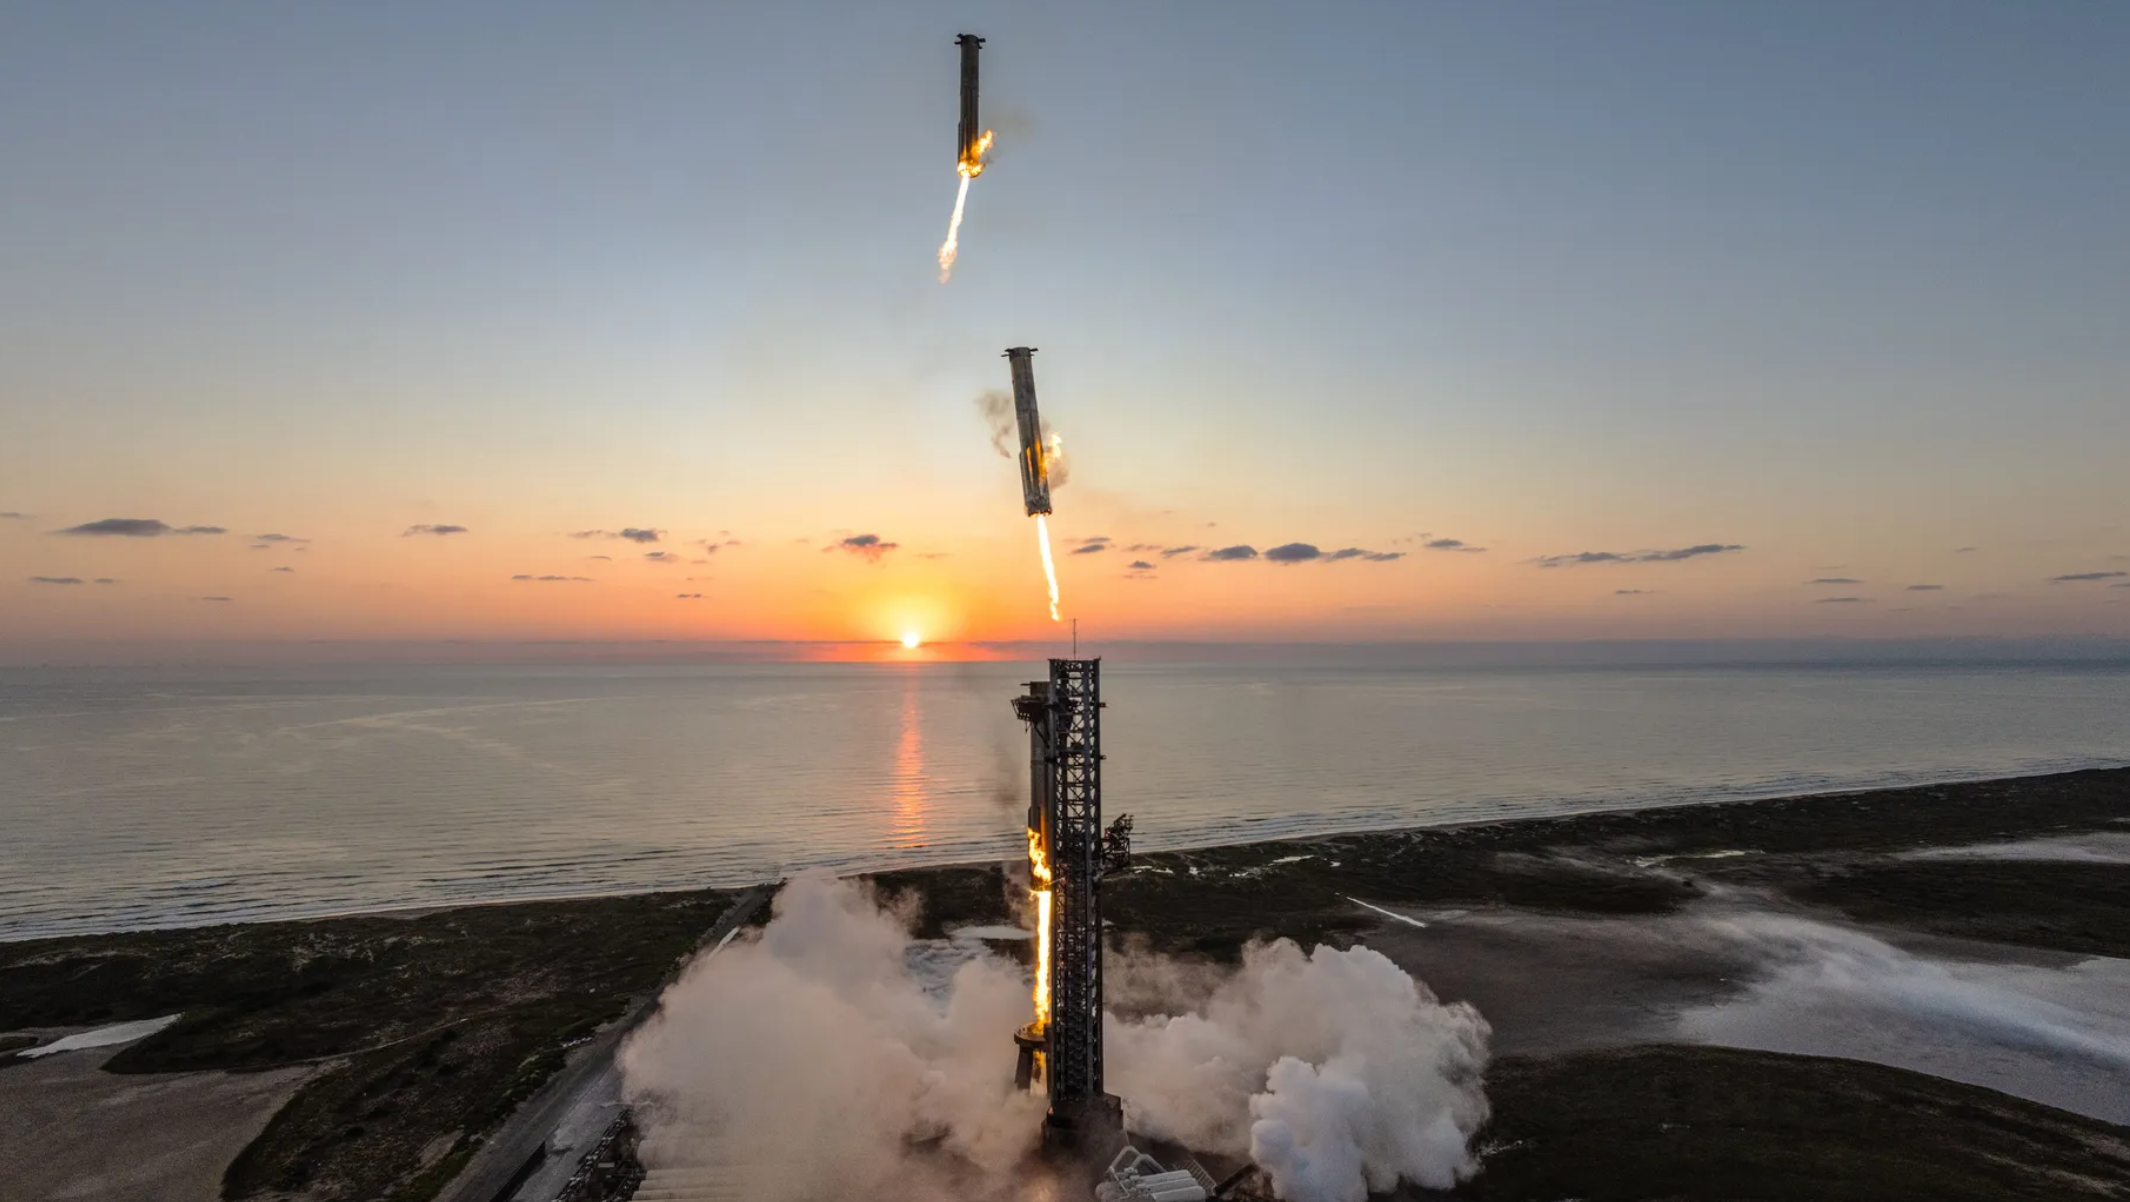
\includegraphics[width=0.85\textwidth]{SpaceX_chopstick_landing.png} \\ \tiny (Image Credit: SpaceX)
    \end{center}
\end{frame}

\begin{frame}{}
    \begin{columns}
    \centering
    \begin{column}{0.5\textwidth}
        \centering
        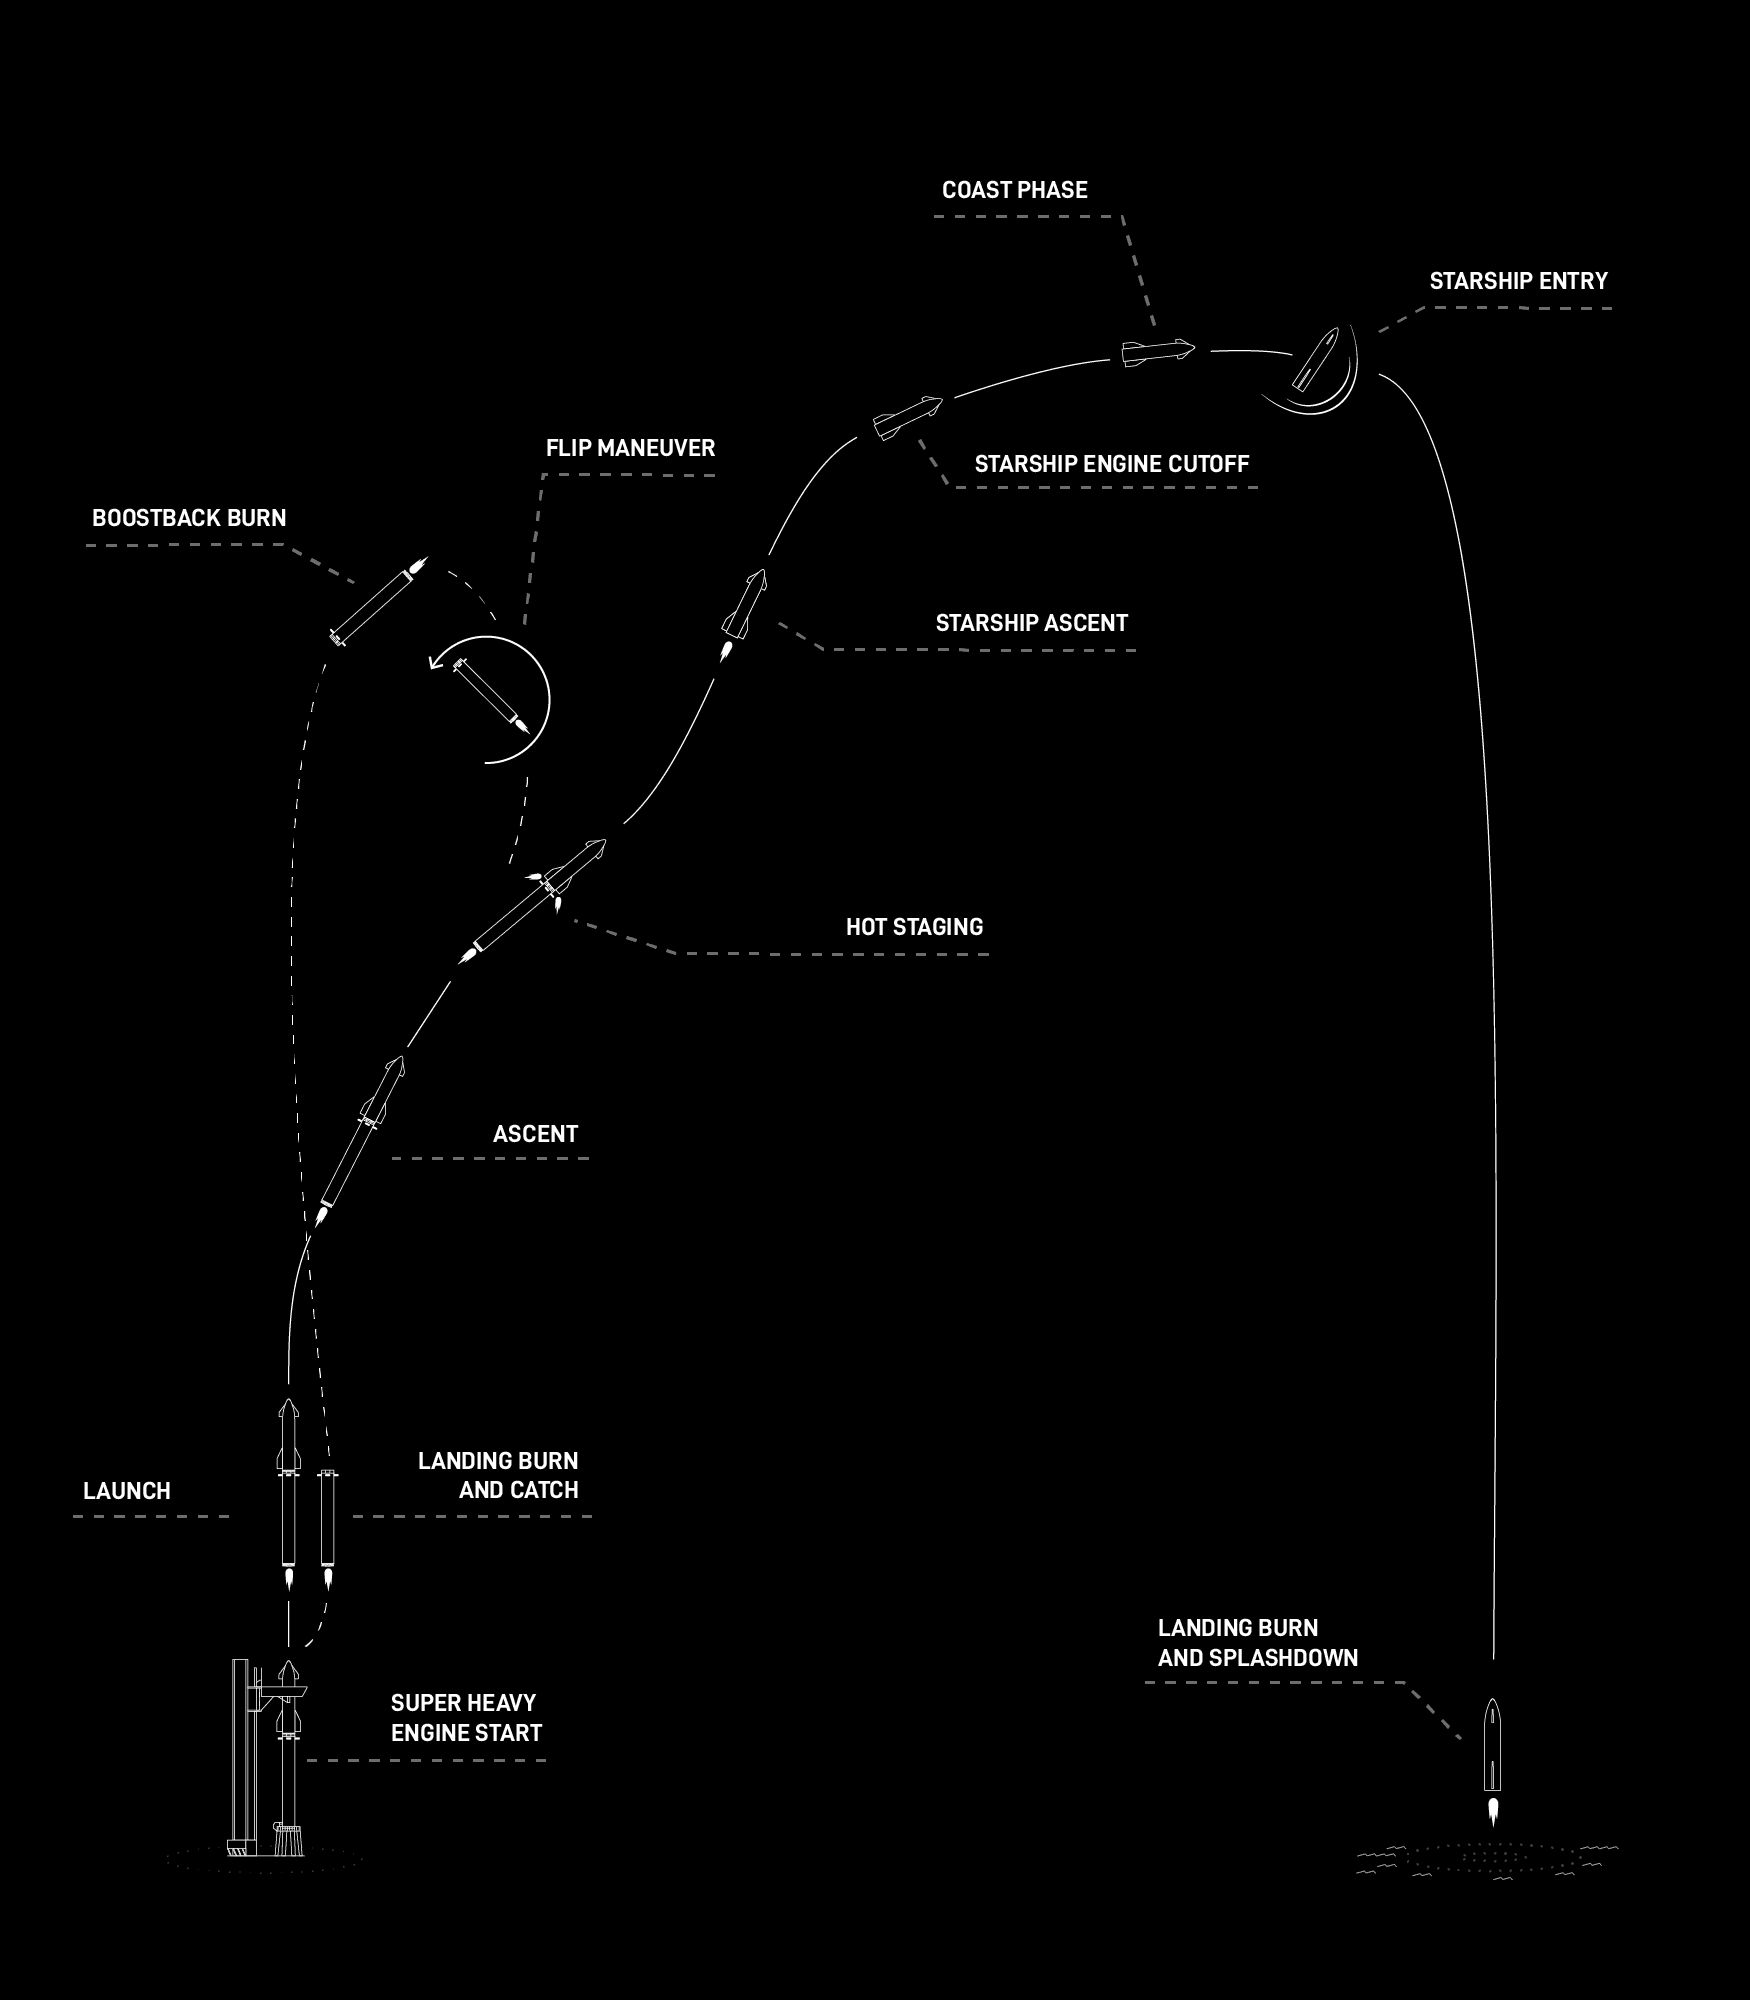
\includegraphics[width=\textwidth]{SPACEX_STARSHIP_INFOGRAPHIC.png}
        \\ \tiny (Image Credit: SpaceX)
    \end{column}
    \begin{column}{0.5\textwidth}
    The launch, flight, and landing paths of the Super Heavy Booster and Starship
    \\[10pt]
    \begin{itemize}
        \item How do they achieve these complex spacecraft maneuvers?
        % landing leg, Grid Fins, multi-engine systems
        % Cold gas Thusters
        % Inertia Navigation System and GPS
        \item<2> More importantly, how do they make sure the rockets \alert{do not deviate} from their course?
        % Many uncertainties (atmospheric disturbance, wind, temperature, model error)
        % It has to know where it is (GPS, Inertia Navigation System)
        % it know deviations from the predefined paths
        % correct its course by 
    \end{itemize}
\end{column}
\end{columns}
\end{frame}

\begin{frame}{Key Systems of SpaceX Reusable Rockets}
    \begin{columns}[t]
        \begin{column}{0.32\textwidth}
            \centering
            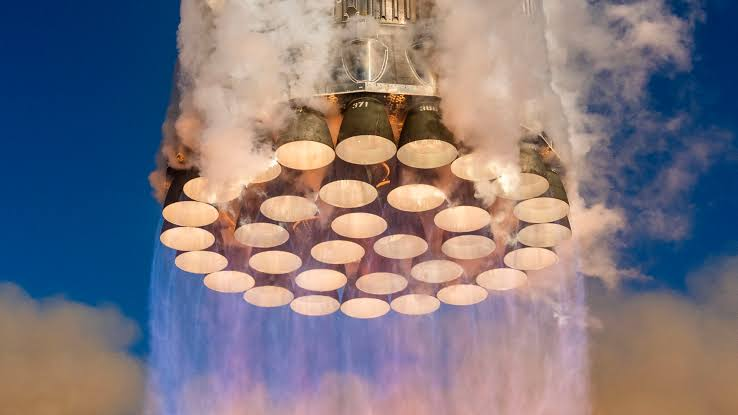
\includegraphics[height=2.5cm]{SpaceX_Boosters.jpeg}\\[4pt]
            \textbf{\small Engine Clusters}\\[2pt]
            {\footnotesize Tilting the engines steers the thrust vector; throttling sets
            its magnitude} % The main actuator in \alert{all} flight phases.}
        \end{column}
        \begin{column}{0.32\textwidth}
            \centering
            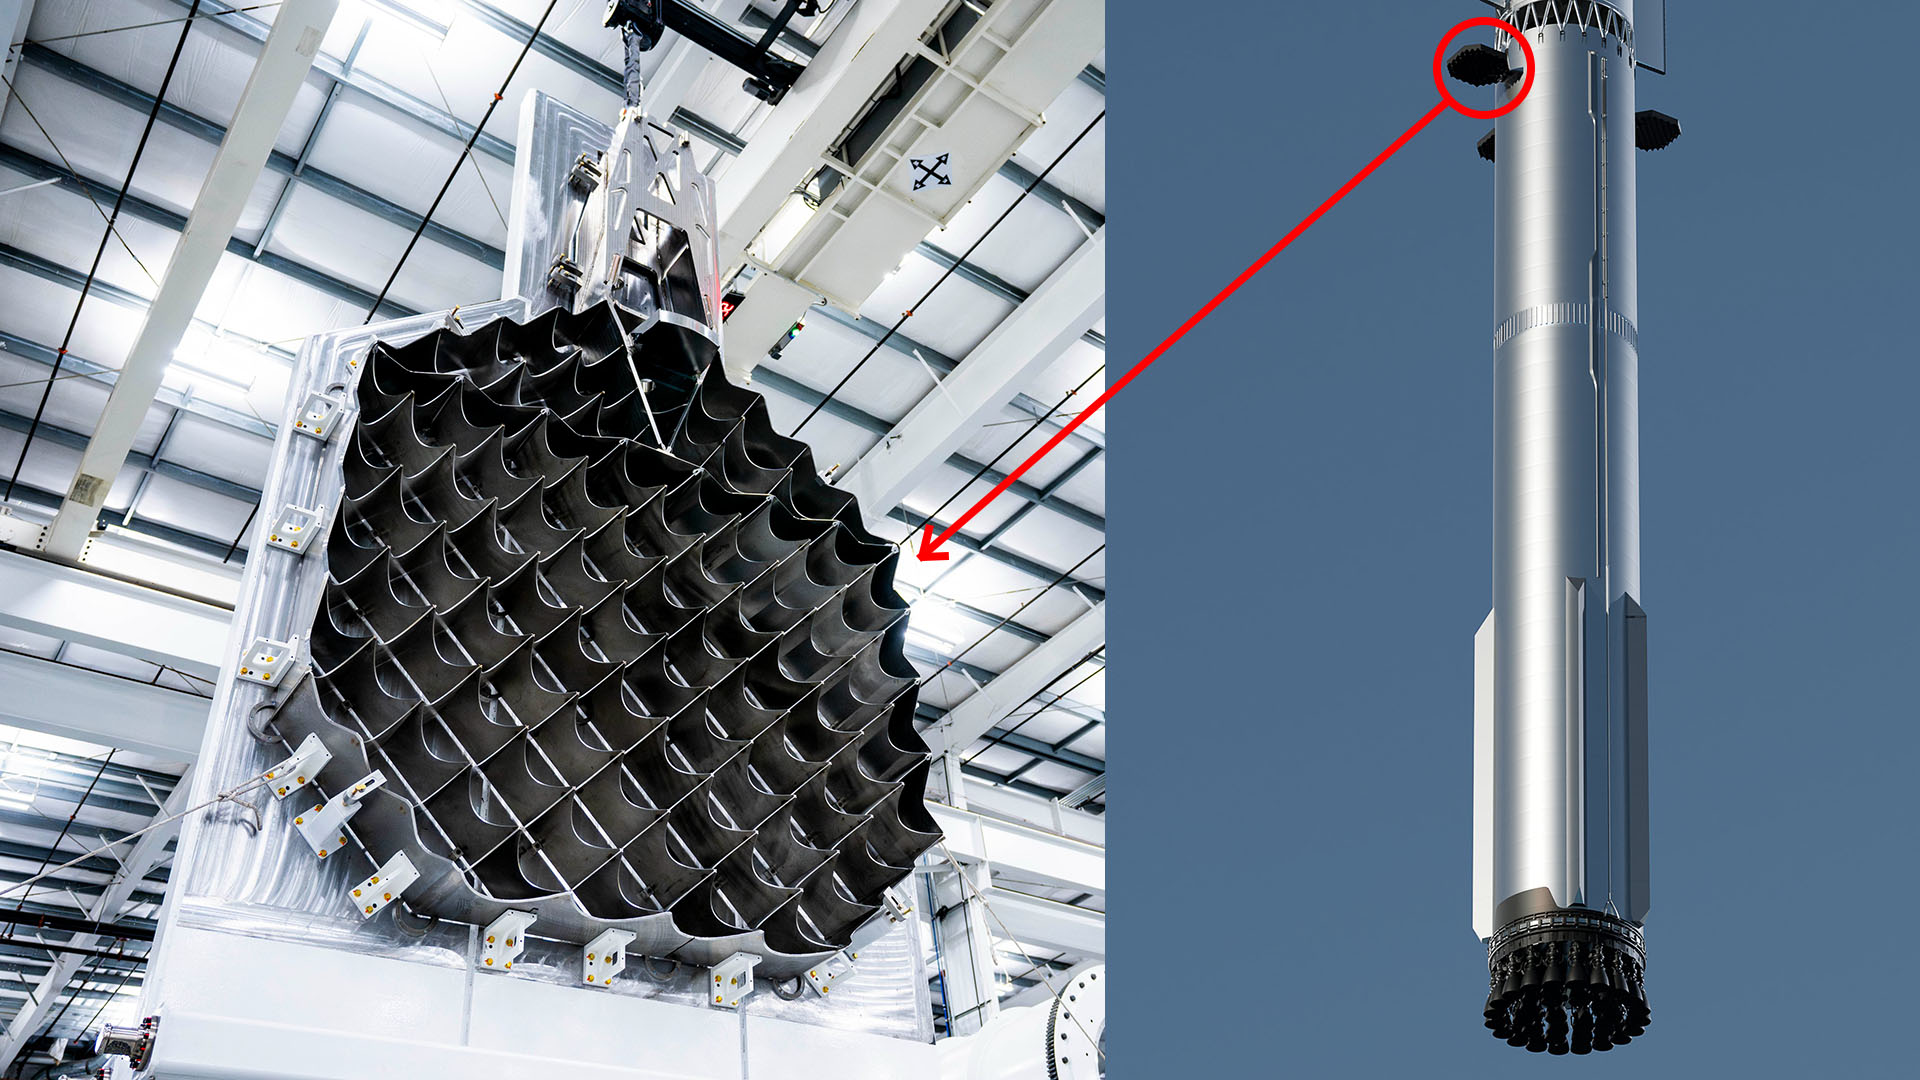
\includegraphics[height=2.5cm]{SpaceX_Super-Heavy-Grid-Fin-Design.jpg}\\[4pt]
            \textbf{\small Grid Fins}\\[2pt]
            {\footnotesize Aerodynamic steering while descending through the thick atmosphere}
            % \alert{thick atmosphere}; they need dynamic pressure to produce any force.}
        \end{column}
        \begin{column}{0.32\textwidth}
            \centering
            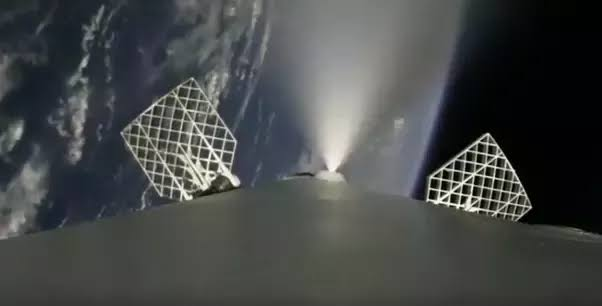
\includegraphics[height=2.5cm]{SpaceX_cold_gas_thruster.jpeg}\\[4pt]
            \textbf{\small Cold-Gas Thrusters}\\[2pt]
            {\footnotesize Attitude control in vacuum}
            %, where fins are useless: the flip maneuver and coasting orientation.}
        \end{column}
    \end{columns}
    \vspace{0.6em}
    
    \begin{center}
        \alert{So, how do they coordinate all these systems to achieve the desired trajectory?}
    \end{center}
    % All three are \alert{actuators}: each has authority in a different flight regime,
    % so the controller must hand over between them.
    \vspace{4pt}

    \blfootnote{\tiny All images credit: SpaceX}
\end{frame}

% --- Anatomy of a control system: built up one component at a time ----
% Running example: the plant is the SpaceX booster.

\begin{frame}{Control System: The Plant}
    \loopPlant[0.95]
    \vspace{0.5em}
    The \alert{plant} (or \alert{process}) is the system we want to control: the rocket.
    \begin{itemize}
        \item Input $u$: the command we can apply (thrust, engine/fin gimbal angle).
        \item Output $y$: what we care about (position, velocity, attitude).
        \item Modeling means writing how $u$ produces $y$.
    \end{itemize}
\end{frame}

\begin{frame}{Control System: Reference and Open-Loop Controller}
    \loopFeedforward[0.82]
    \vspace{0.5em}
    Add the \alert{reference} $r$ (desired trajectory) and a \alert{controller} that
    turns it into $u$.
    \begin{itemize}
        \item Purely \alert{feedforward}: commands pre-scheduled before flight.
        \item \alert{Open-loop}: nothing measures the state of the rocket. 
        \item Works only if the model is perfect and the world is predictable.
    \end{itemize}
\end{frame}

\begin{frame}{Control System: Disturbance}
    \loopDisturbance[0.75]
    \vspace{0.5em}
    A \alert{disturbance} $d$ acts on the plant.
    \begin{itemize}
        \item External: wind gusts, air density, unmodeled aerodynamics.
        \item Internal: model uncertainty, e.g.\ mass and CG shifting as propellant burns.
        \item Feedforward alone never corrects the resulting error.
    \end{itemize}
\end{frame}

\begin{frame}{Control System: Feedback and Closed-Loop Controller}
    \loopFeedback[0.70]
    \vspace{0.3em}
    Close the loop with a \alert{sensor} and a \alert{comparator}.
    \begin{itemize}
        \item The sensor (IMU, GPS) reports the measured output $y_m$.
        \item The error $e = r - y_m$ drives the controller: \alert{closed-loop} control.
        \item Feedback rejects $d$ despite an imperfect model.
    \end{itemize}
\end{frame}

\begin{frame}{Control System: Inside the Plant}
    \loopActuatorPlant[0.65]
    \vspace{0.3em}
    Split the plant into the parts we model separately.
    \begin{itemize}
        \item \alert{Actuator}: command $\to$ force or torque (engines, fins, thrusters).
        \item \alert{Dynamic system}: rigid-body dynamics of the rocket.
        \item $d$ is added to the command entering the actuator.
    \end{itemize}
\end{frame}

\begin{frame}{Control System: Measurement Noise}
    \loopNoise[0.65]
    \vspace{0.3em}
    Every measurement is corrupted by \alert{noise} $n$.
    \begin{itemize}
        \item Sensor bias, drift, quantization, vibration.
        \item The controller sees $r - (y + n)$: it reacts to noise as if it were error.
        \item Trade-off: fast feedback tracks better but amplifies noise.
    \end{itemize}
\end{frame}

\begin{frame}{Control System: Summary}
    \loopSummary[0.70]
    \vspace{0.2em}
    \begin{columns}[t]
        \begin{column}{0.48\textwidth}
            \begin{tabular}{@{}r@{\;\;}l@{}}
                $r$:   & reference (desired output) \\
                $e$:   & error, $e = r - y_m$ \\
                $u$:   & control command \\
                $f$:   & actuator force or torque (effort) \\
            \end{tabular}
        \end{column}
        \begin{column}{0.48\textwidth}
            \begin{tabular}{@{}r@{\;\;}l@{}}
                $d$:   & disturbance \\
                $y$:   & actual output \\
                $n$:   & measurement noise \\
                $y_m$: & measured output, $y_m = y + n$ \\
            \end{tabular}
        \end{column}
    \end{columns}
\end{frame}

\begin{frame}{A Simplified Rocket Stabilization Analogy}
    \centering
    The Furuta Pendulum (AKA Rotational Inverted Pendulum)
    \begin{columns}
        \begin{column}{0.33\textwidth}
            \centering
            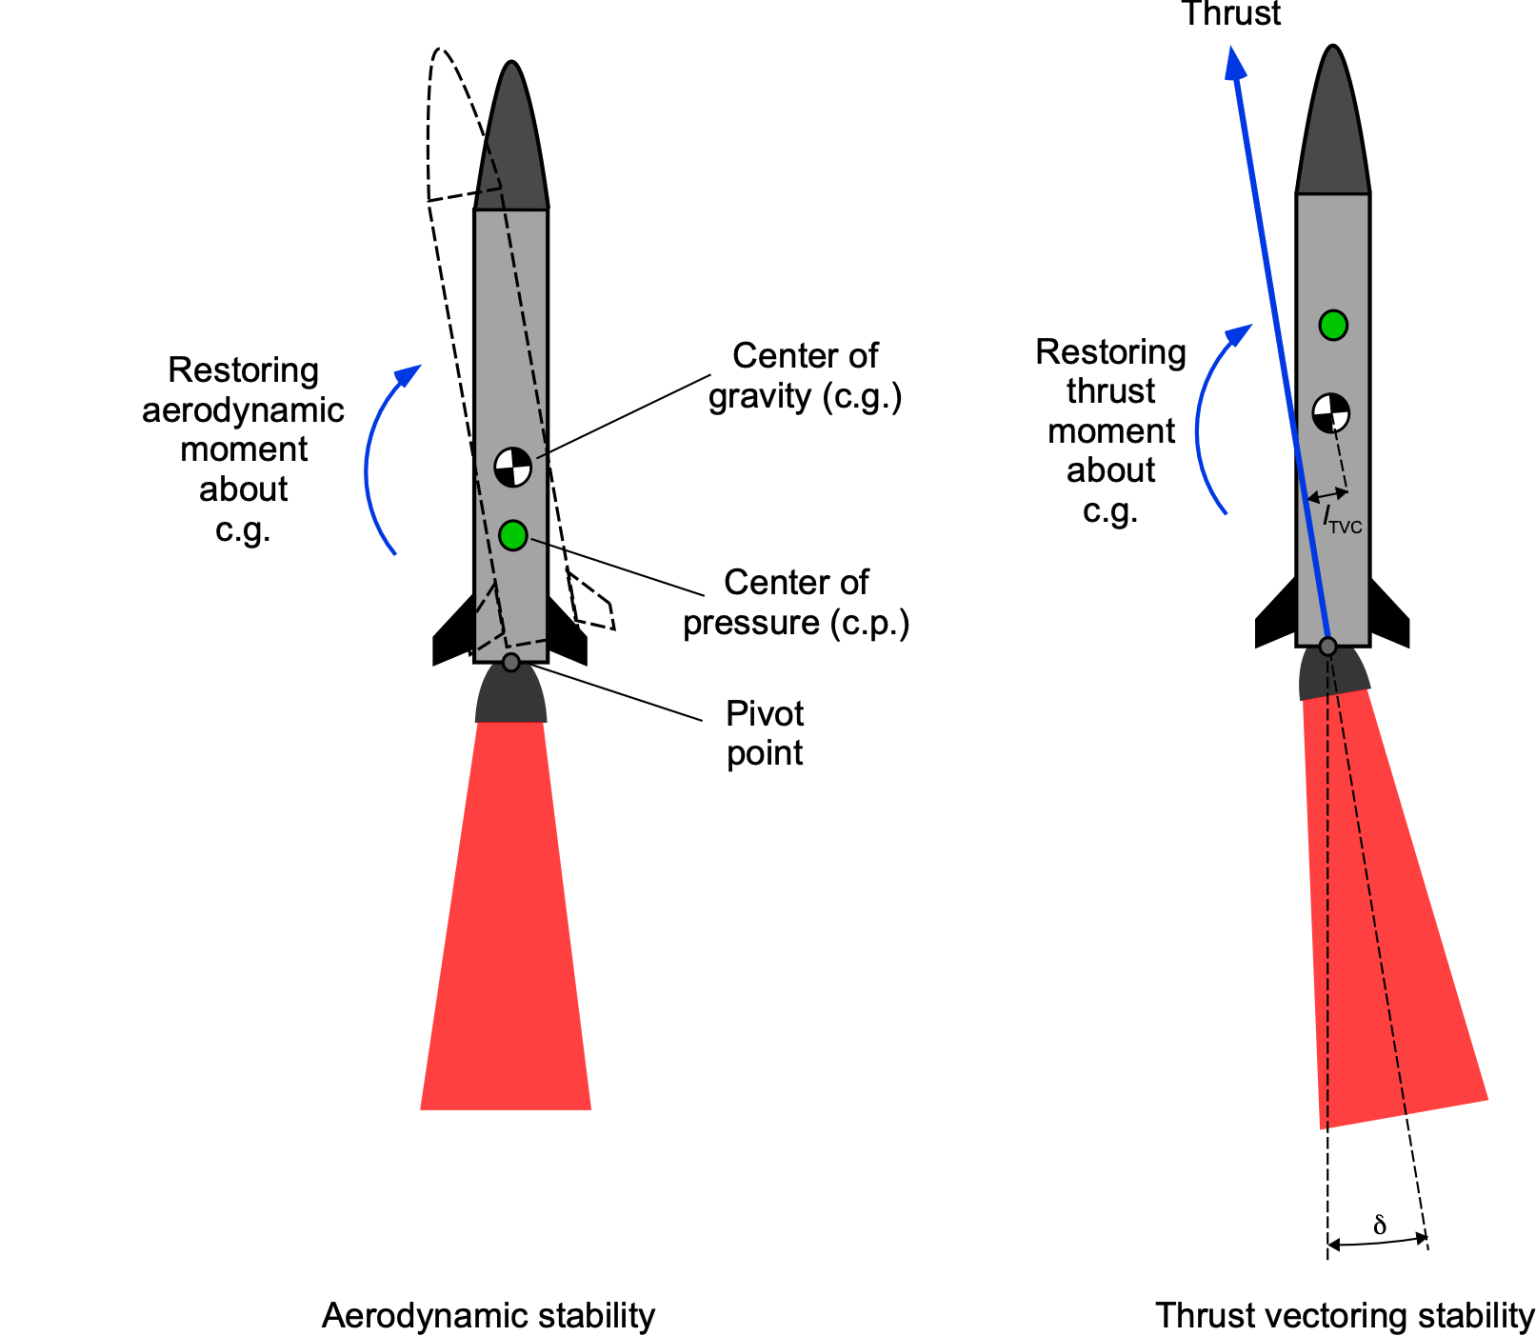
\includegraphics[height=3.5cm]{rocket_stability.png} \\ \tiny (Image Credit: \href{https://eaglepubs.erau.edu/introductiontoaerospaceflightvehicles/chapter/rocket-performance/stability-and-control/}{Introduction to Aerospace Flight Vehicles, J. Gordon Leishman, 2026})
        \end{column}
        \begin{column}{0.33\textwidth}
            \centering
            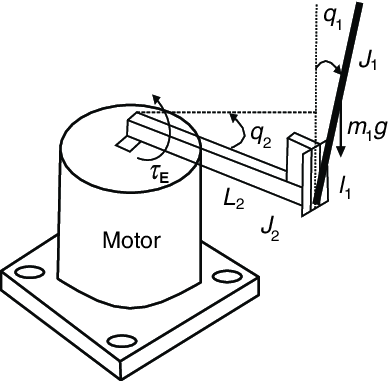
\includegraphics[height=3.5cm]{The-Furuta-pendulum.png} \\ \tiny (Image Credit: Aguilar-Ibáñez et al., 2010)
        \end{column}
        \begin{column}{0.33\textwidth}
            \centering
            \includegraphics[height=3.5cm]{furuta_pendulum_auto_control_II_project.png}
            \\ \tiny (Project by Namo Ekpattharasakul, \href{https://youtu.be/qtClAbNr92E?si=gUyduqwmFPXvqZYV}{YouTube Video})
        \end{column}
    \end{columns}
    % demo video of Furuta Pendulum (opens in the system's default player)
    \begin{center}
       \small \movie[externalviewer]{\alert{$\blacktriangleright$~Play Video: Furuta Pendulum Control Demo (.mp4)}}{videos/furuta_pendulum_demo.mp4}
    \end{center}
    What are the Actuator, Plant, Sensor, Controller, Reference, Disturbance, and Noise in this system?
    % Aguilar-Ibáñez, Carlos & Suárez-Castañón, Miguel & Gutiérres-Frias, Oscar. (2010). The direct Lyapunov method for the stabilisation of the Furuta pendulum. International Journal of Control. 83. 2285-2293. 10.1080/00207179.2010.520029. 
\end{frame}

\begin{frame}{}
    \centering
    \Large What are the advantages and disadvantages of \newline \textbf{open-loop} vs \textbf{closed-loop} control?
\end{frame}

\begin{frame}{Open-Loop vs Closed-Loop}
    \begin{columns}[t]
        \begin{column}{0.5\textwidth}
            \textbf{Open-loop (feedforward)}
            \begin{itemize}
                \item[\textcolor{brandred}{$+$}] Simple and cheap: no sensor needed
                \item[\textcolor{brandred}{$-$}] Cannot detect or correct error
                \item[\textcolor{brandred}{$-$}] Fails under disturbance or model error
            \end{itemize}
        \end{column}
        \pause
        \begin{column}{0.5\textwidth}
            \textbf{Closed-loop (feedback)}
                \begin{itemize}
                    \item[\textcolor{brandred}{$+$}] Stability: can stabilize an unstable plant
                    \item[\textcolor{brandred}{$+$}] Performance: precisely tracks reference and rejects disturbance
                    \item[\textcolor{brandred}{$+$}] Automation: reduces human intervention
                    \item[\textcolor{brandred}{$-$}] Needs sensors, actuators, and controllers: more complex and costly
                    % \item[\textcolor{brandred}{$-$}] Feeds measurement noise back into the loop
                \end{itemize}
        \end{column}
    \end{columns}
    \vspace{1em}
    \pause
    \begin{center}
        \alert{Feedback is not free}: a badly designed loop oscillates or diverges (\alert{Instability}).\\
        Guaranteeing \alert{stability} comes first, performance second.
    \end{center}
\end{frame}

\begin{frame}
    \begin{center}
        \Large What are \textbf{Control Systems} in our everyday life?
    % airflyer / oven
    \end{center}
\end{frame}

\begin{frame}{Control Systems Are Everywhere}
    % Pictures of
    % Elevator Mechanism (elevator_mechanism.png)(Elevator Mechanism. Source: DENIS Starostin / Getty Images)
    % Air Conditioners (air_conditioner.jpeg) (Air Conditioner. Source: KangeStudio / Getty Images)
    % Crane (tower_crane.jpeg)(Tower Crane. Source: goldenwingsphotography / Getty Images)
    % Autonomous Car (waymo_self-driving_car.jpeg)(Source: Waymo)
    % Drones (Quadcopter_camera_dront_in_flight.jpeg)(canrail / Getty Images)
    %  Process Plants (process_plant.jpeg) (Process Plant. Source: nui7711 / Getty Images)
    \vspace{0.3em}
    \begin{columns}[c]
        \begin{column}{0.30\textwidth}
            \centering
            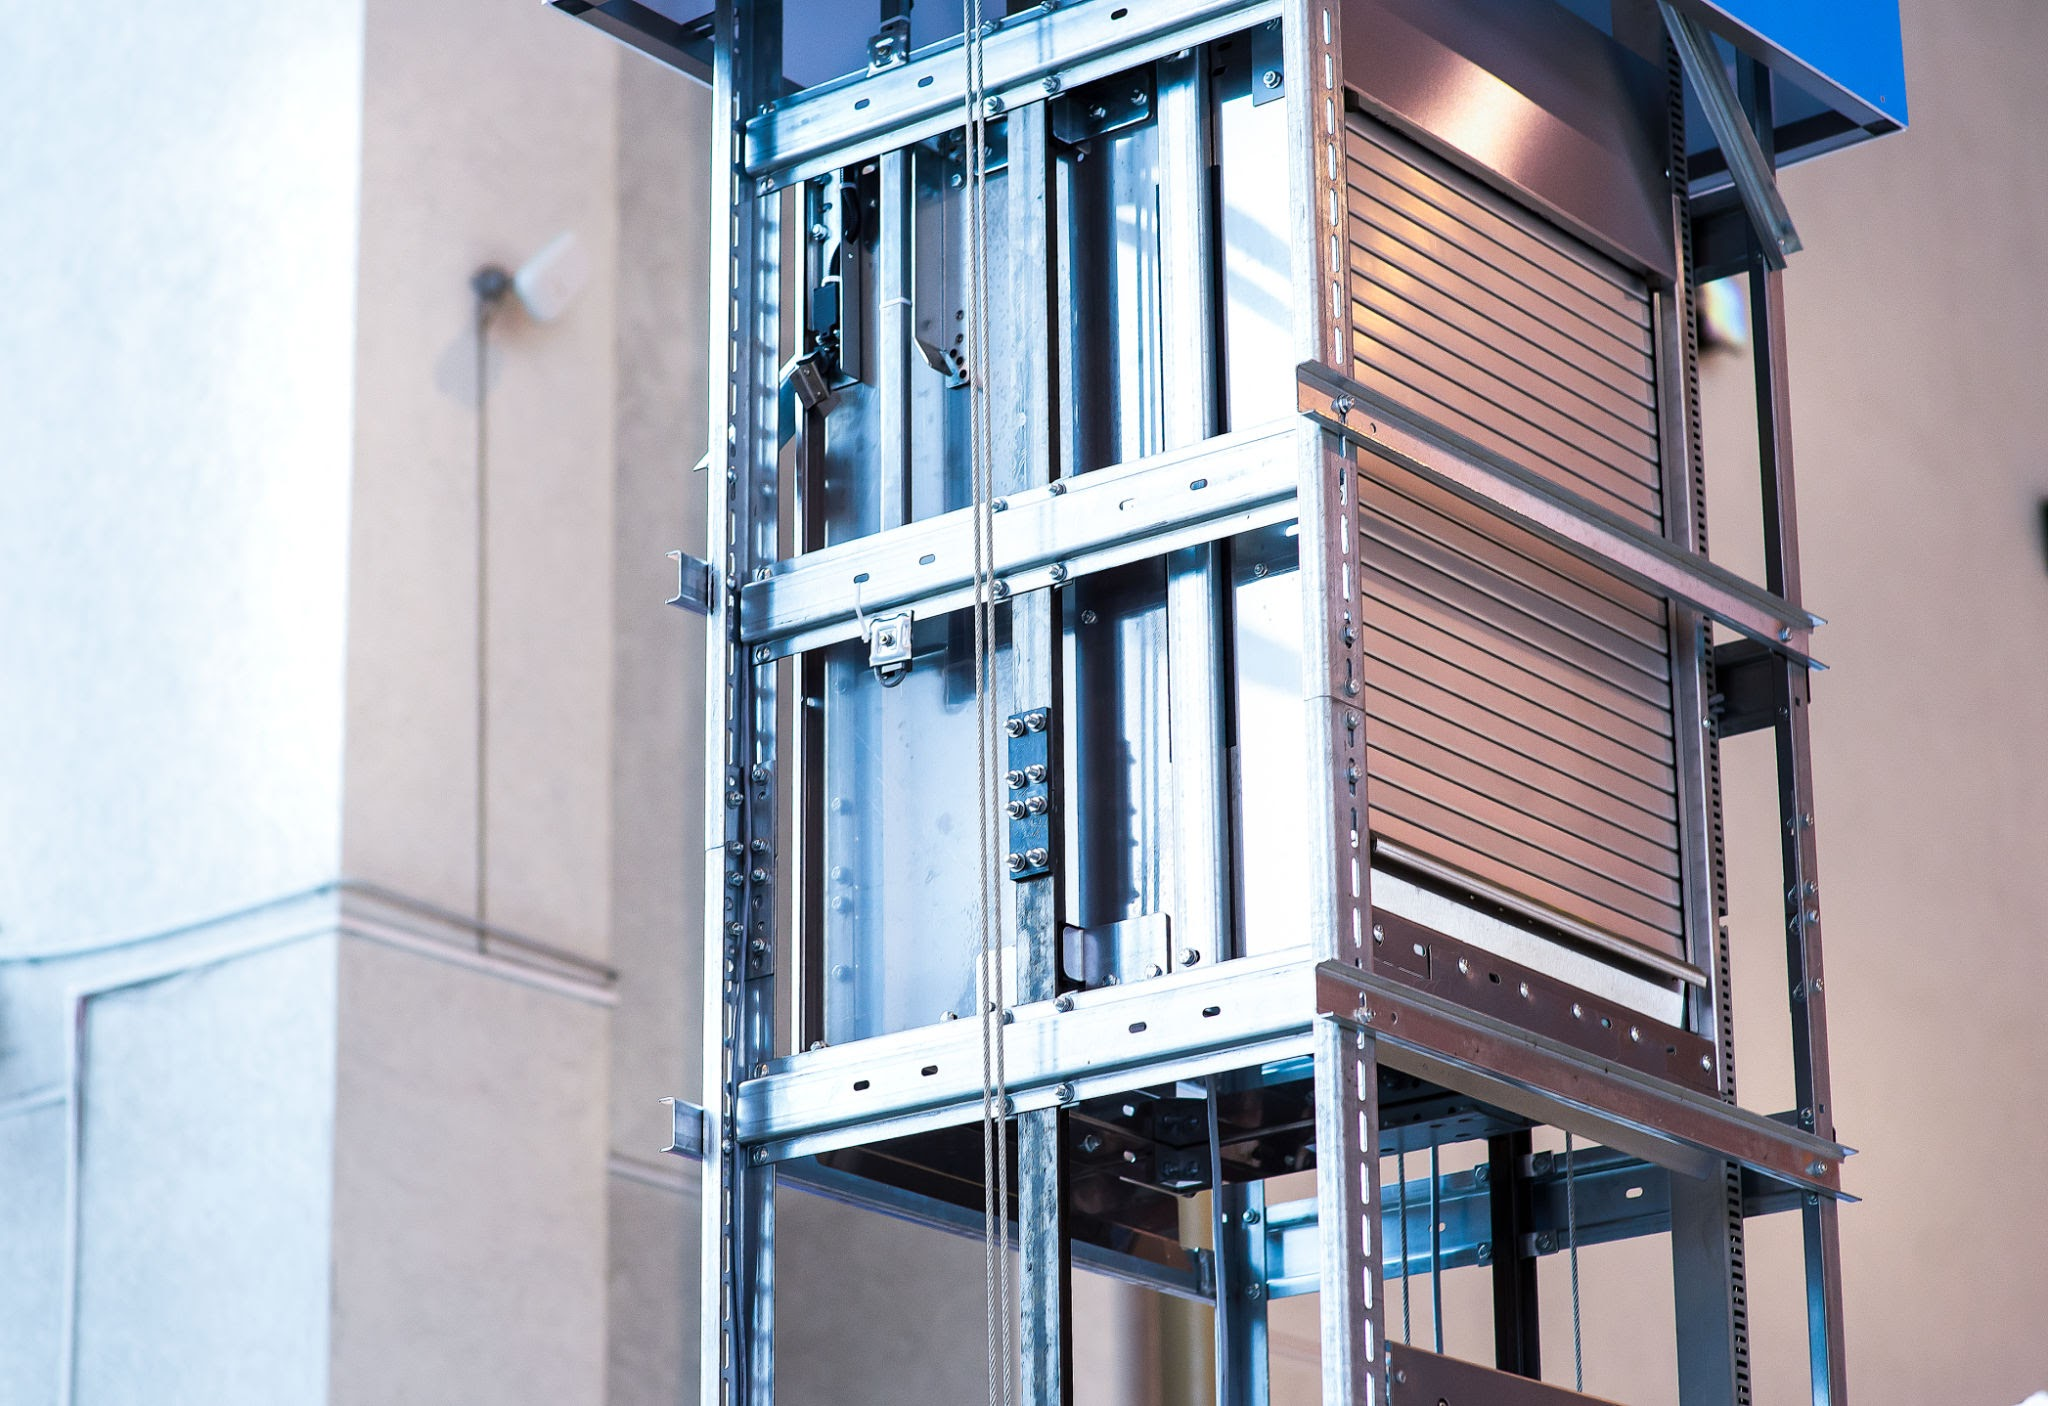
\includegraphics[width=\linewidth, height=2.5cm, keepaspectratio]{elevator_mechanism.jpeg}\\[3pt]
            {\small Elevator}
        \end{column}
        \begin{column}{0.30\textwidth}
            \centering
            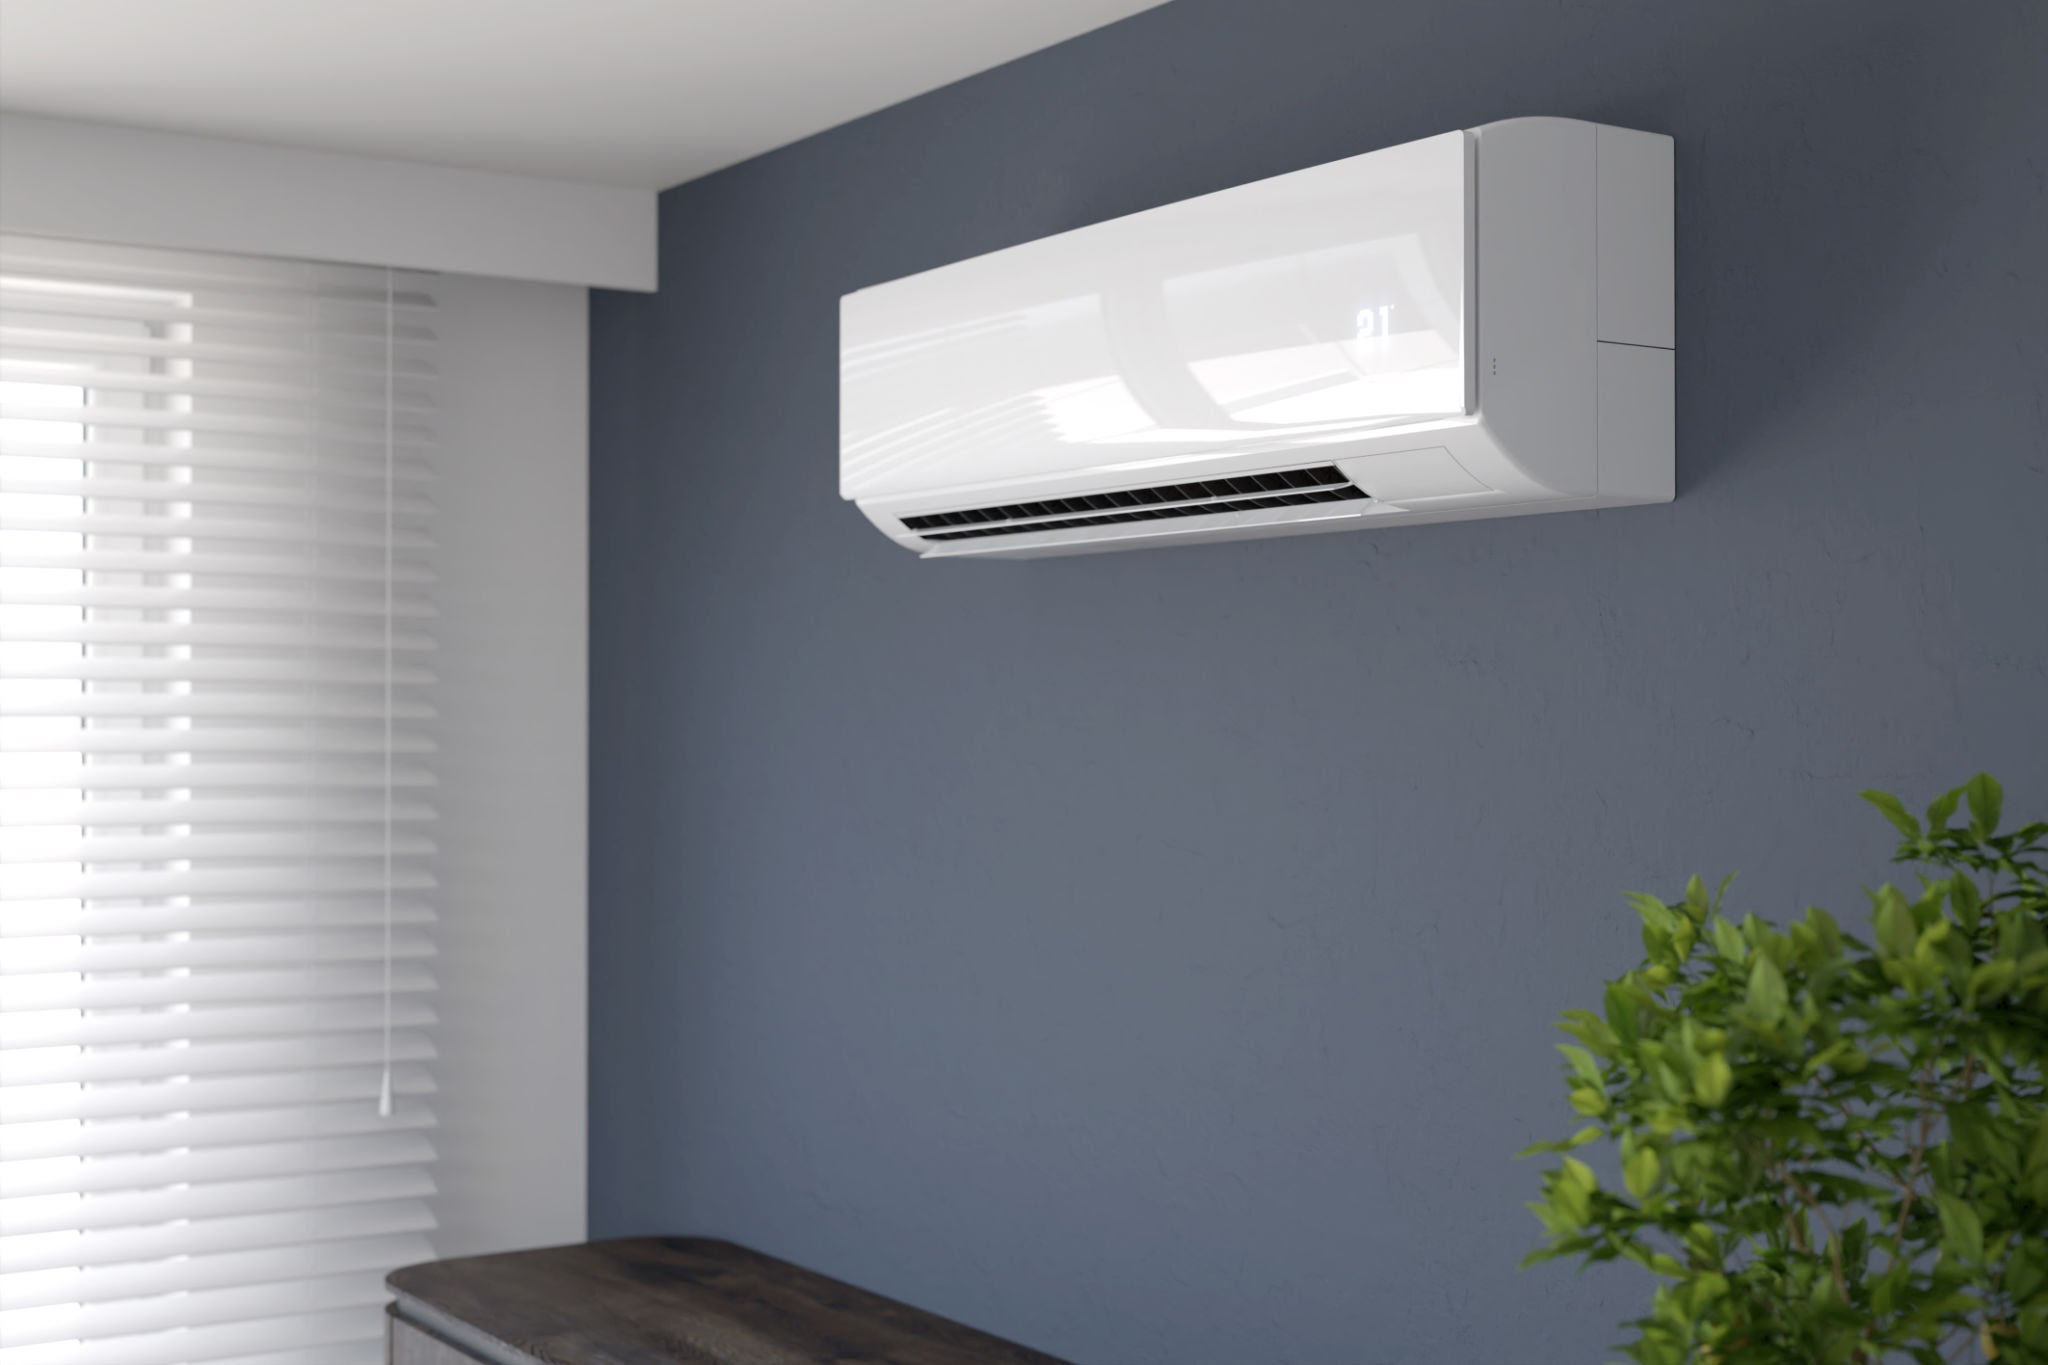
\includegraphics[width=\linewidth, height=2.5cm, keepaspectratio]{air-conditioner.jpeg}\\[3pt]
            {\small Air Conditioner}
        \end{column}
        \begin{column}{0.30\textwidth}
            \centering
            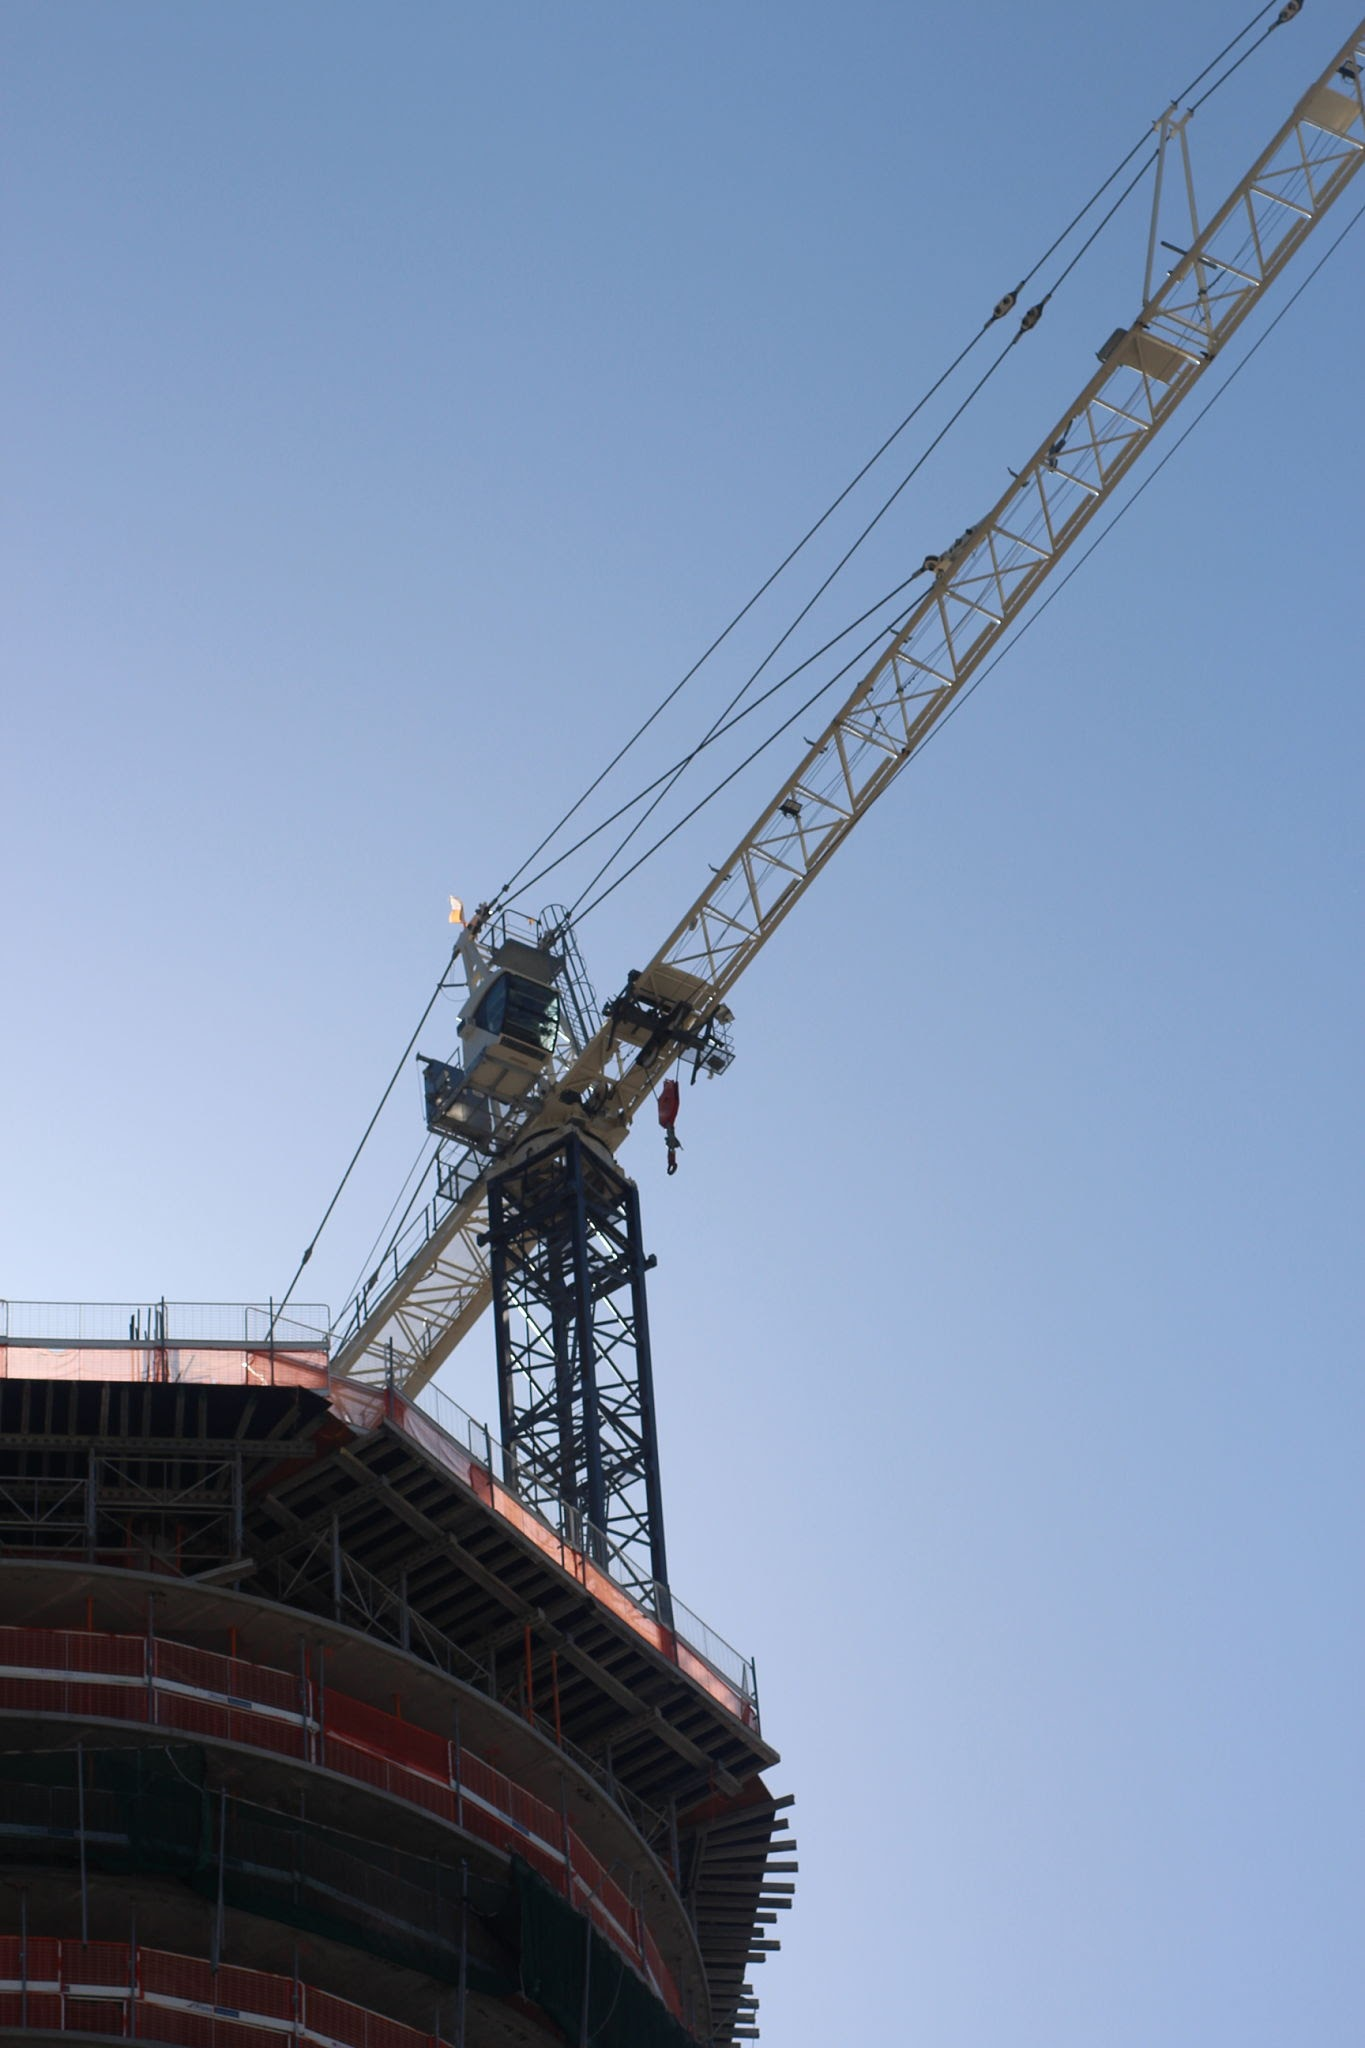
\includegraphics[width=\linewidth, height=2.5cm, keepaspectratio]{tower_crane.jpeg}\\[3pt]
            {\small Tower Crane}
        \end{column}
    \end{columns}
    \vspace{0.6em}
    \begin{columns}[c]
        \begin{column}{0.30\textwidth}
            \centering
            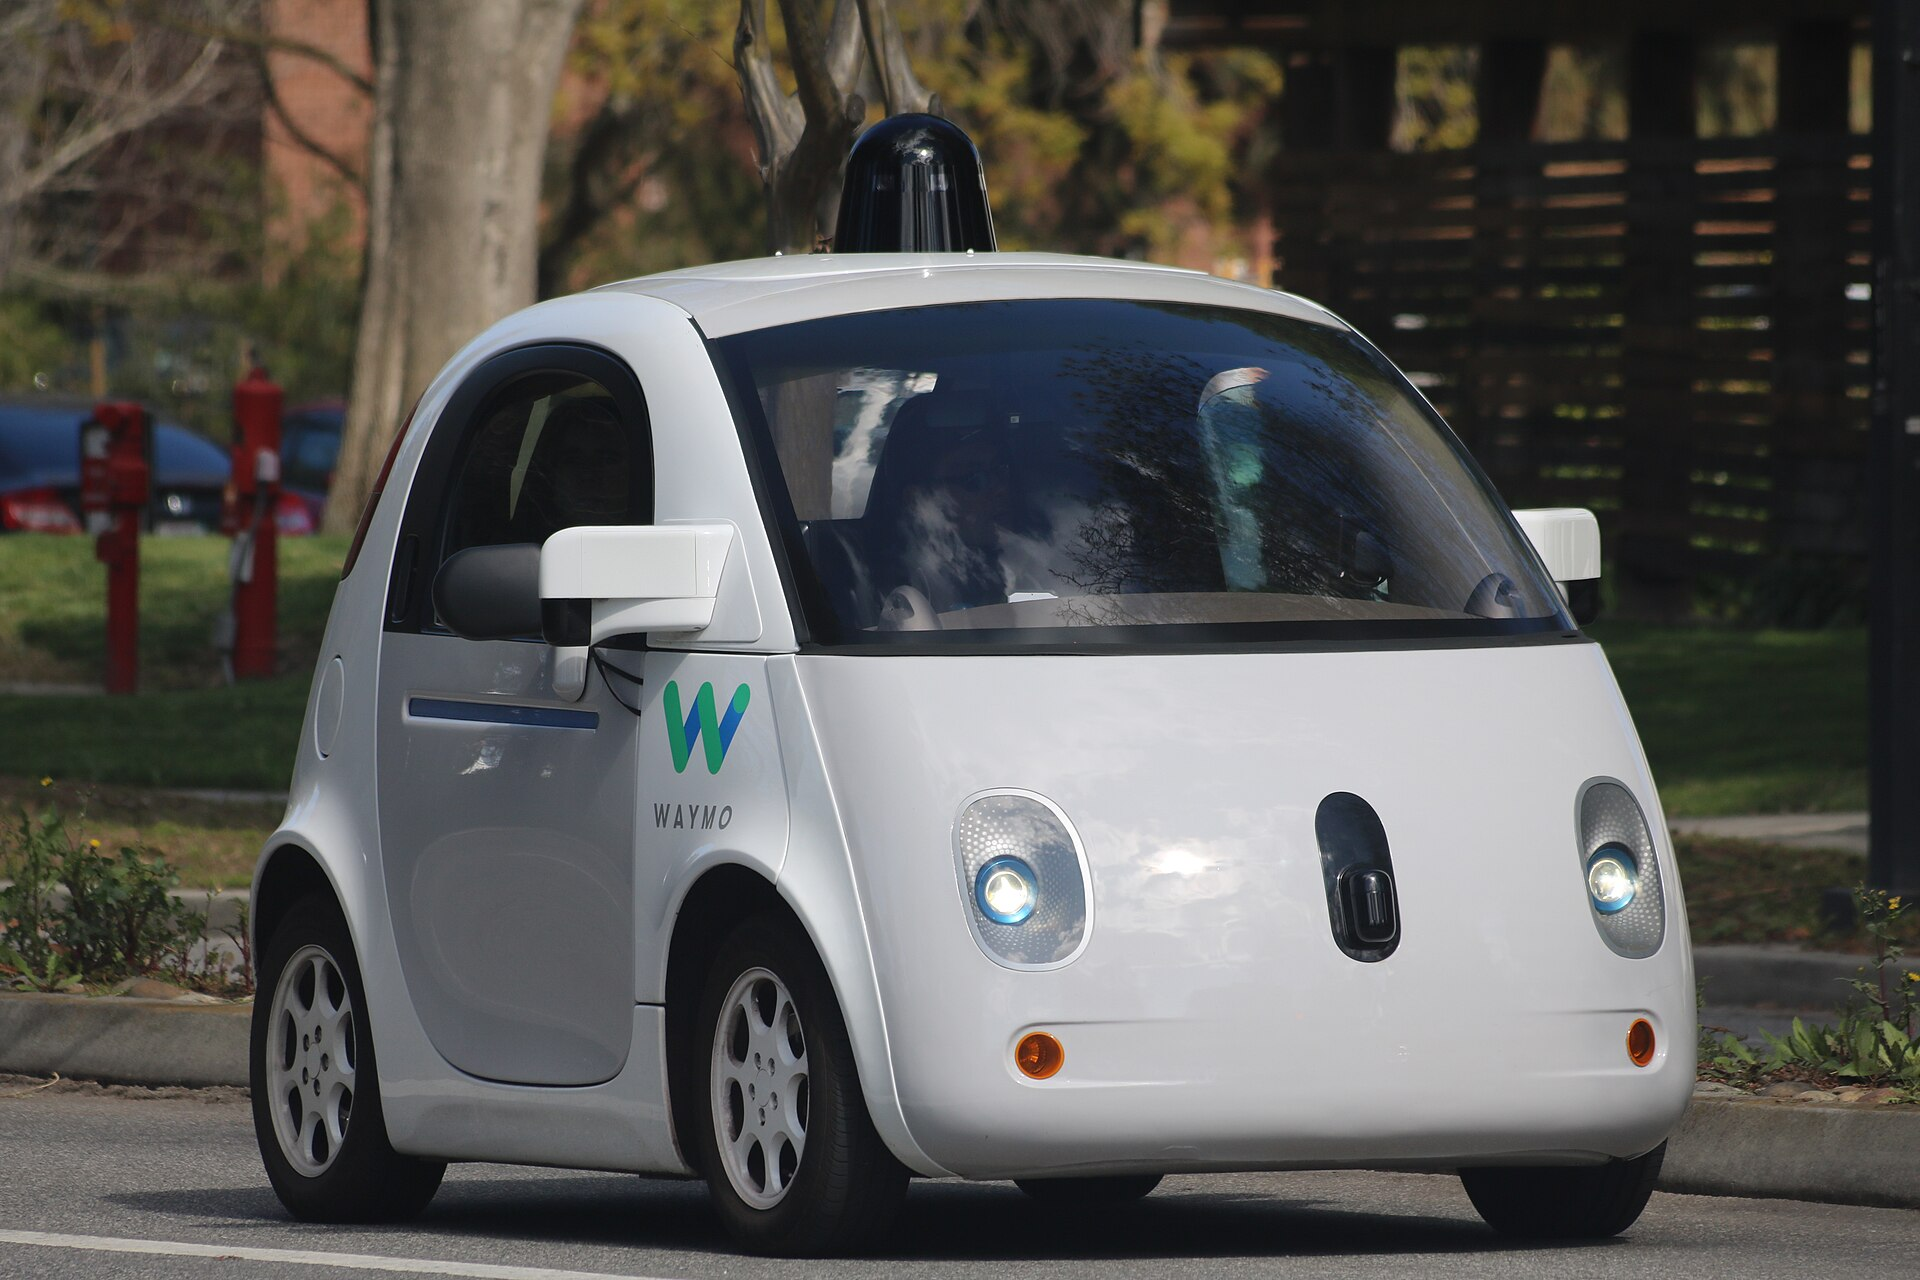
\includegraphics[width=\linewidth, height=2.5cm, keepaspectratio]{Waymo_self-driving_car_front_view.gk.jpg}\\[3pt]
            {\small Autonomous Car}
        \end{column}
        \begin{column}{0.30\textwidth}
            \centering
            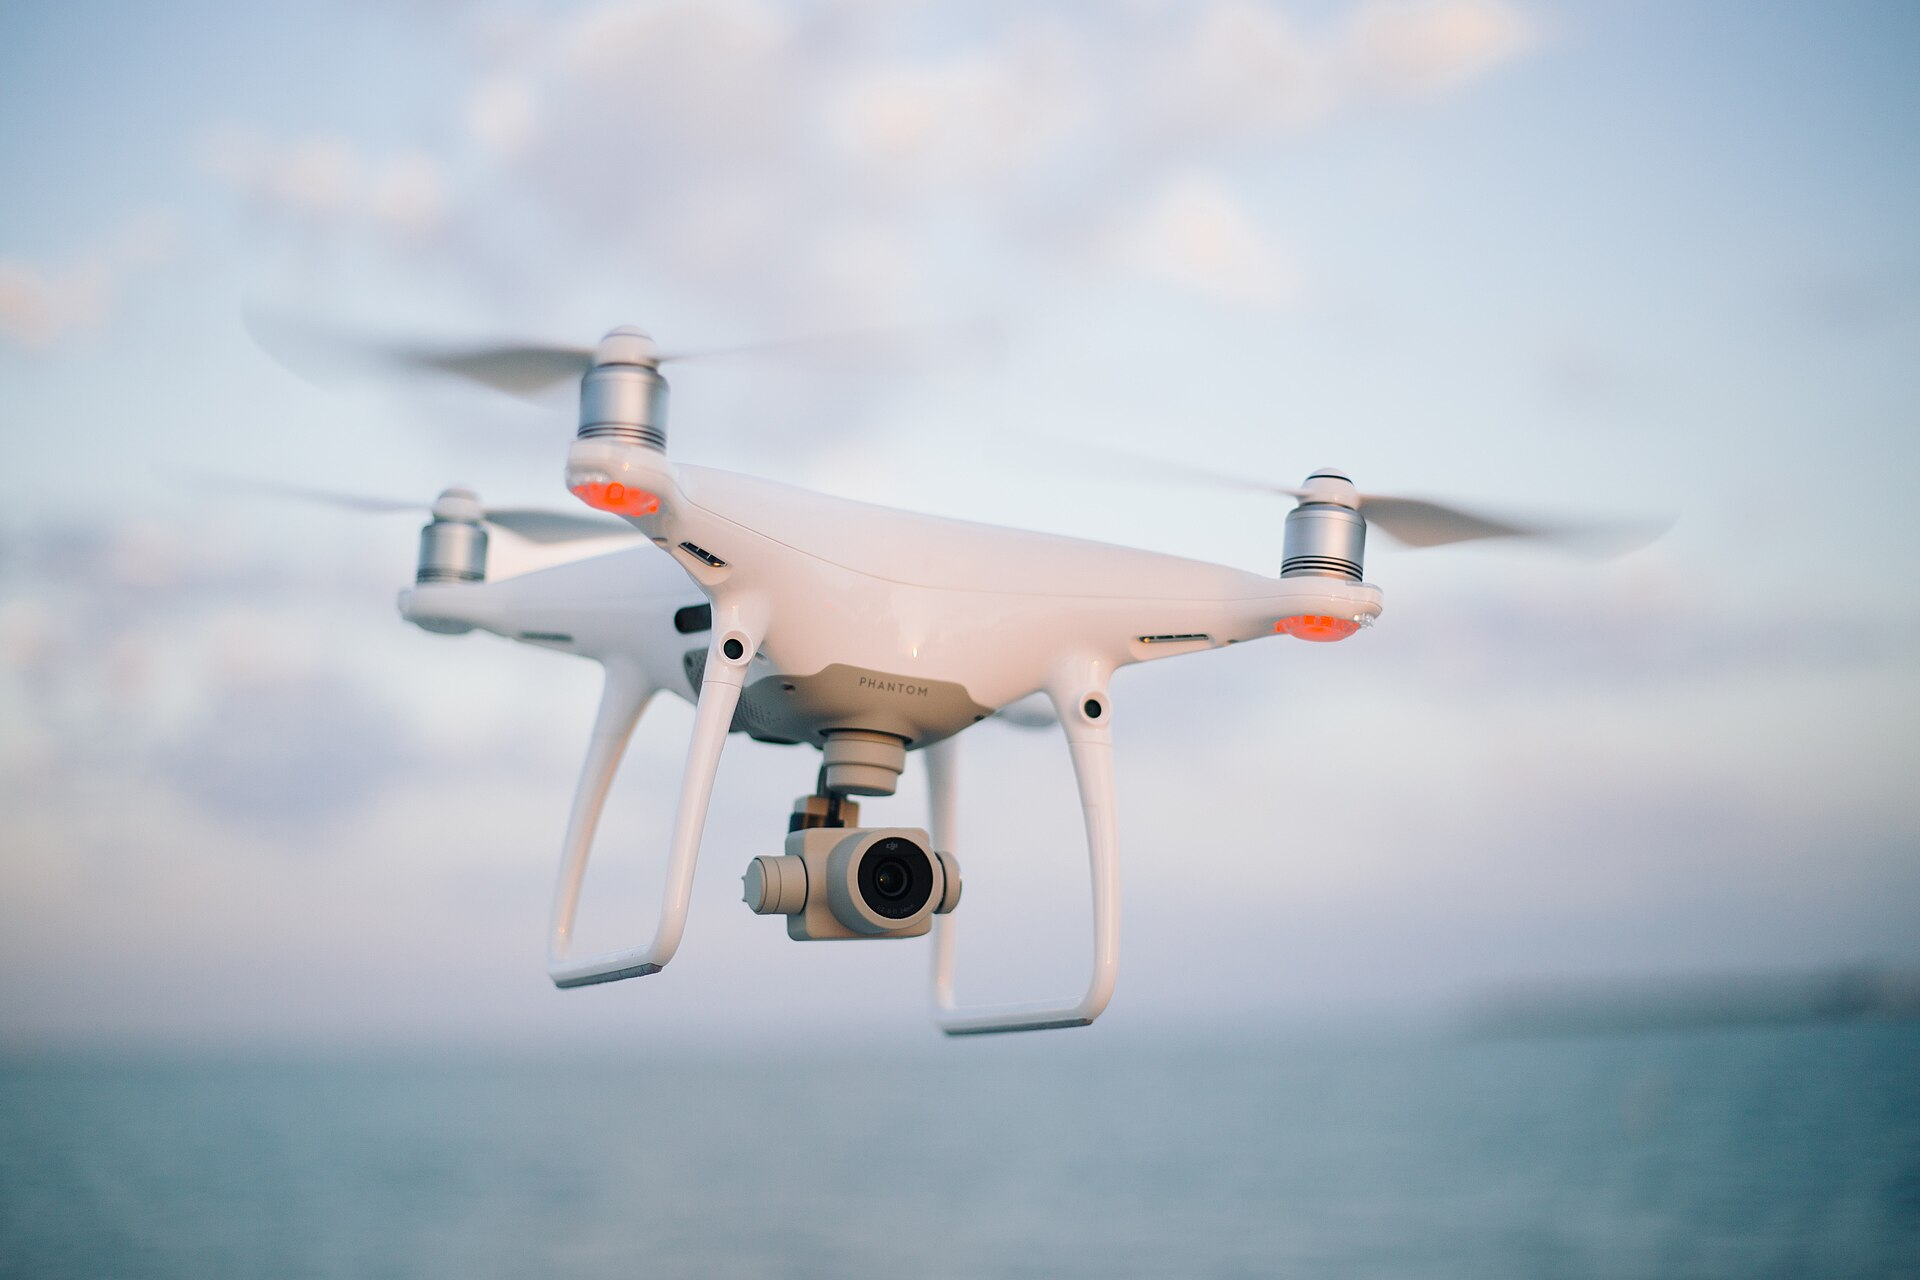
\includegraphics[width=\linewidth, height=2.5cm, keepaspectratio]{Quadcopter_camera_drone_in_flight.jpg}\\[3pt]
            {\small Drone}
        \end{column}
        \begin{column}{0.30\textwidth}
            \centering
            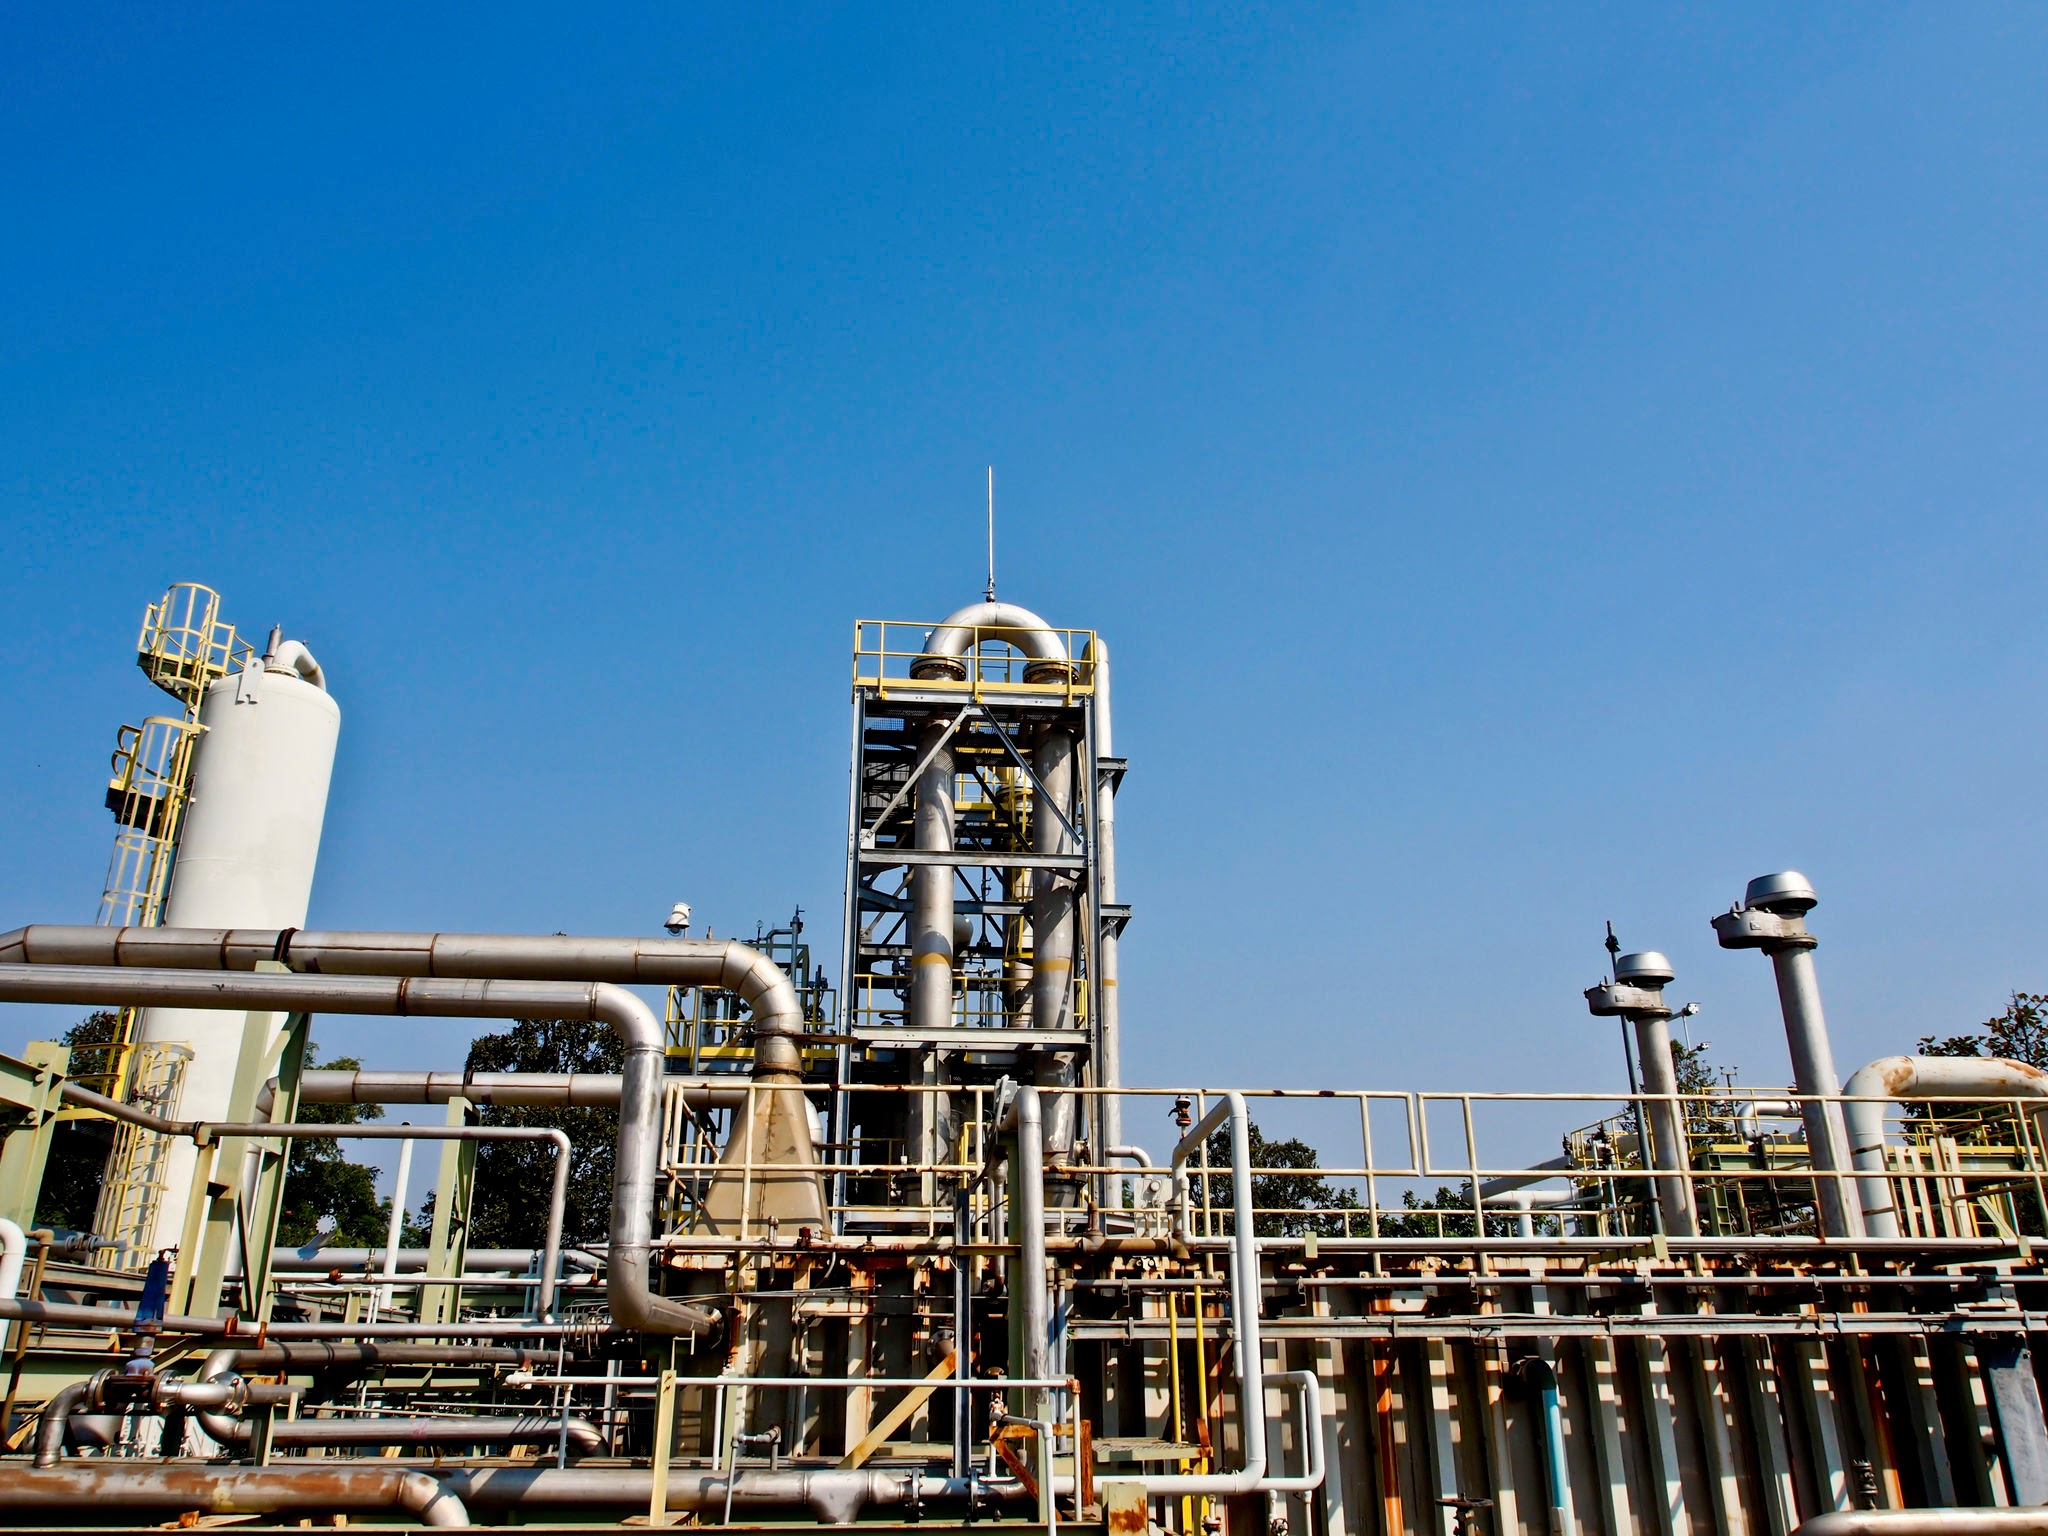
\includegraphics[width=\linewidth, height=2.5cm, keepaspectratio]{process_plant.jpeg}\\[3pt]
            {\small Process Plant}
        \end{column}
    \end{columns}
    \blfootnote{\tiny Image credits: Elevator: DENIS Starostin / Getty Images;
        Air conditioner: KangeStudio / Getty Images;
        Tower crane: goldenwingsphotography / Getty Images;
        Autonomous car: Waymo; Drone: canrail / Getty Images;
        Process plant: nui7711 / Getty Images}
\end{frame}

\begin{frame}{Control Systems Are Everywhere}
    % industrial_robot.jpeg (Industrial Robotic Arm. Source: Mihajlo Maricic / Getty Images)
    % Humanoid Robots (Atlas Robot. Source: Boston Dynamics)
    % Surgical Robots (Da Vinci, Surgical Robot. Source: Intuitive Surgical)
    % XoMotion_exoskeleton (XoMotion, The World's Most Advanced Exoskeleton. (CNW Group/Human in Motion Robotics Inc.))
    \vspace{0.5em}
    \begin{columns}[T]
        \begin{column}{0.23\textwidth}
            \centering
            \parbox[c][3.7cm][c]{\linewidth}{\centering
                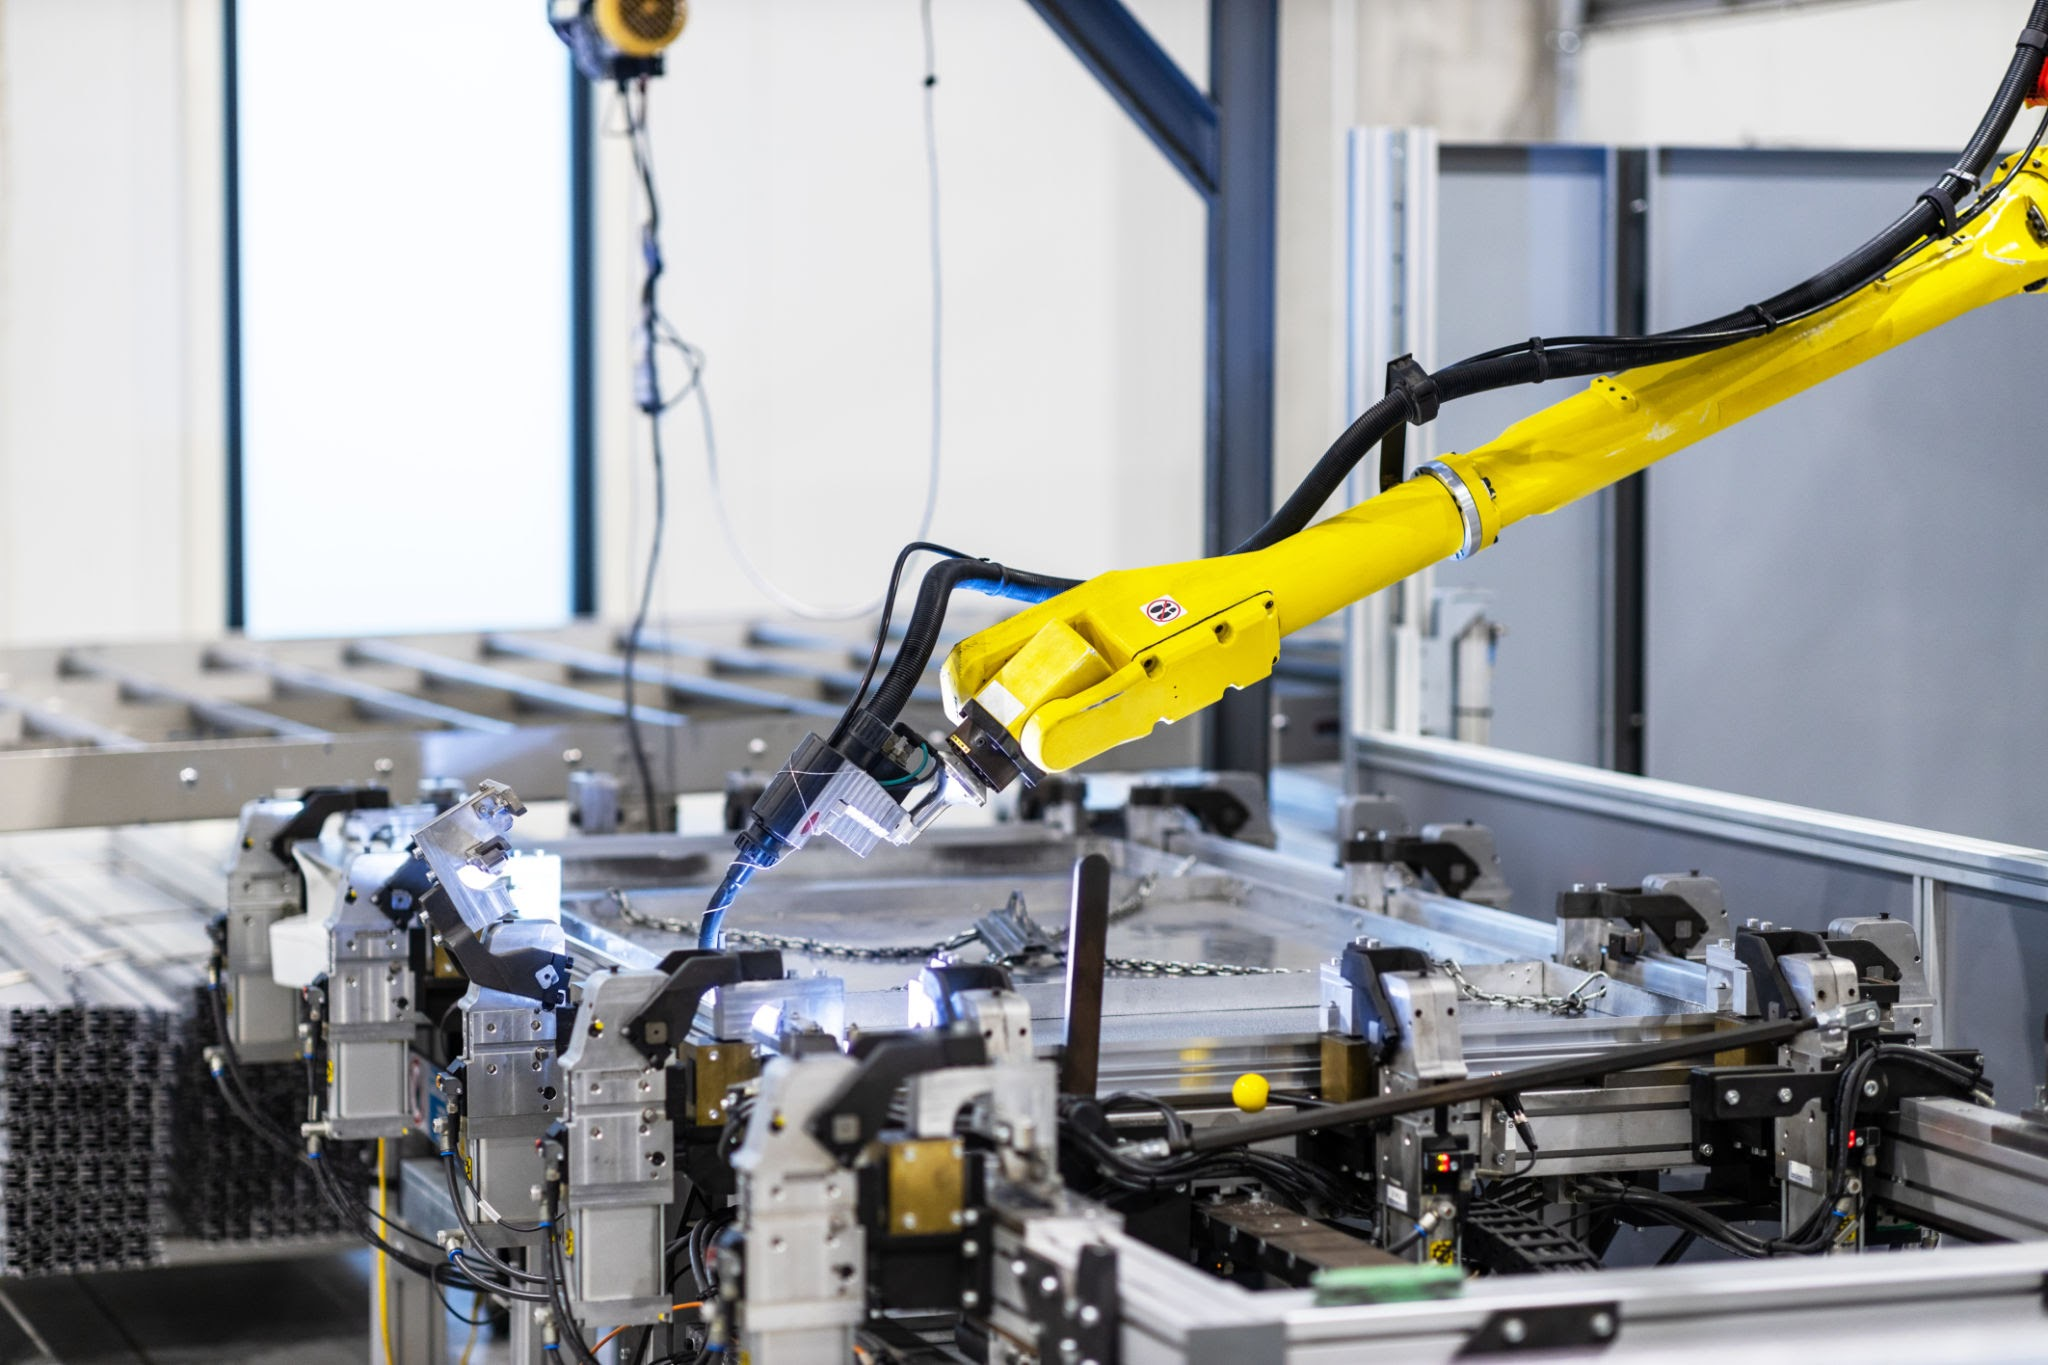
\includegraphics[width=\linewidth, height=4.25cm, keepaspectratio]{industrial_robot.jpeg}}\\[3pt]
            {\small Industrial Robot}
        \end{column}
        \begin{column}{0.23\textwidth}
            \centering
            \parbox[c][3.7cm][c]{\linewidth}{\centering
                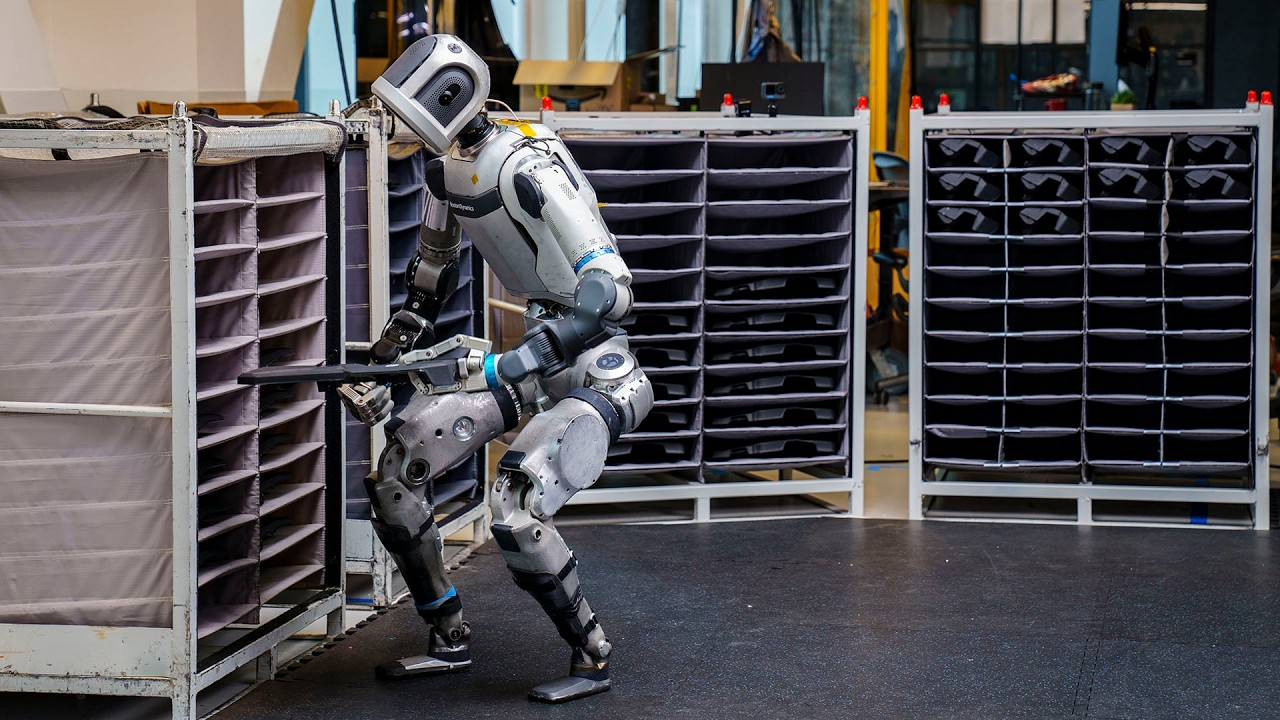
\includegraphics[width=\linewidth, height=4.25cm, keepaspectratio]{atlas_robot_working.jpg}}\\[3pt]
            {\small Humanoid Robot}
        \end{column}
        \begin{column}{0.23\textwidth}
            \centering
            \parbox[c][3.7cm][c]{\linewidth}{\centering
                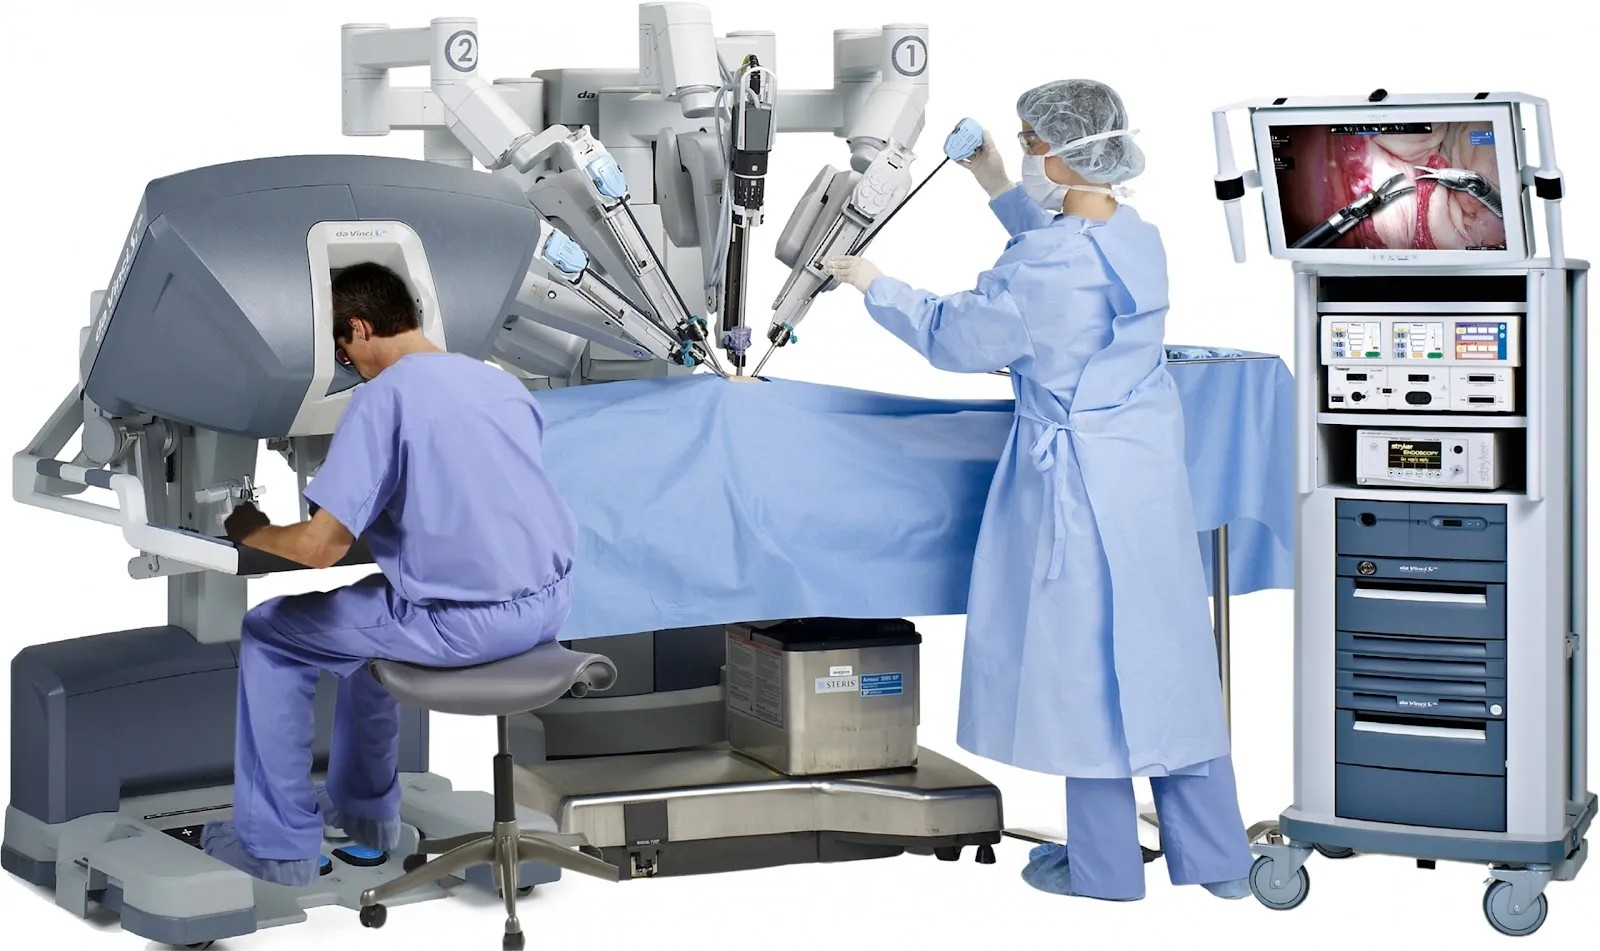
\includegraphics[width=\linewidth, height=4.25cm, keepaspectratio]{davinci_robot.jpeg}}\\[3pt]
            {\small Surgical Robot}
        \end{column}
        \begin{column}{0.23\textwidth}
            \centering
            \parbox[c][3.7cm][c]{\linewidth}{\centering
                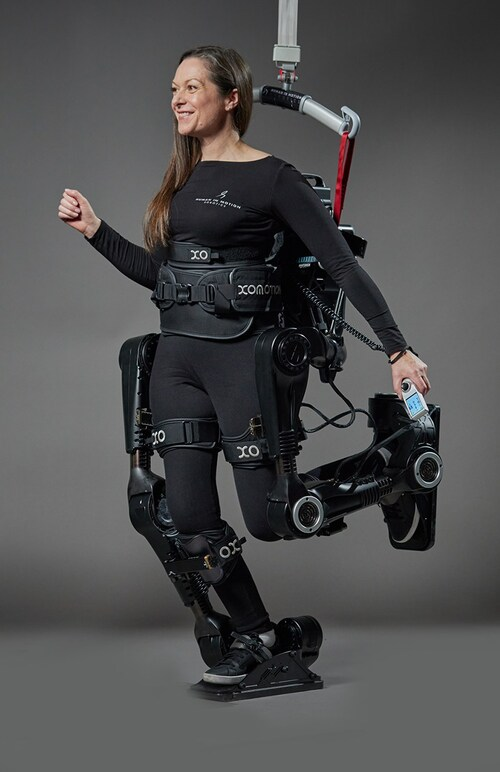
\includegraphics[width=\linewidth, height=3.8cm, keepaspectratio]{XoMotion_exokeleton.jpg}}\\[3pt]
            {\small Exoskeleton}
        \end{column}
    \end{columns}
    \blfootnote{\tiny Image credits: Industrial robotic arm: Mihajlo Maricic / Getty Images;
        Atlas robot: Boston Dynamics; da Vinci surgical robot: Intuitive Surgical;
        XoMotion exoskeleton: CNW Group / Human in Motion Robotics Inc.}
\end{frame}

% \begin{frame}{Brief History of Automatic Control Systems}
    % \begin{itemize}
    %     \item 1788: James Watt's centrifugal governor for steam engines
    %     \item 1868: Maxwell's mathematical analysis of governors
    %     \item 1922: Nyquist's stability criterion
    %     \item 1930s: Bode's frequency response methods
    %     \item 1940s: State-space methods and optimal control
    %     \item 1950s: Digital control and computer-aided design
    %     \item 1960s: Modern control theory and robust control
    %     \item 1970s: Adaptive control and nonlinear control
    %     \item 1980s: Fuzzy control and neural networks
    %     \item 1990s: Intelligent control and hybrid systems
    %     \item 2000s: Networked control systems and cyber-physical systems
    % \end{itemize}
% \end{frame}

\begin{frame}{The Very First Automatic Feedback Control System}
    James Watt's \alert{flyball governor} (1769): holds the speed of a steam engine
    constant, entirely mechanically, with no electronics or computer.
    \vspace{1em}
    \begin{columns}[c]
        \begin{column}{0.5\textwidth}
            \centering
            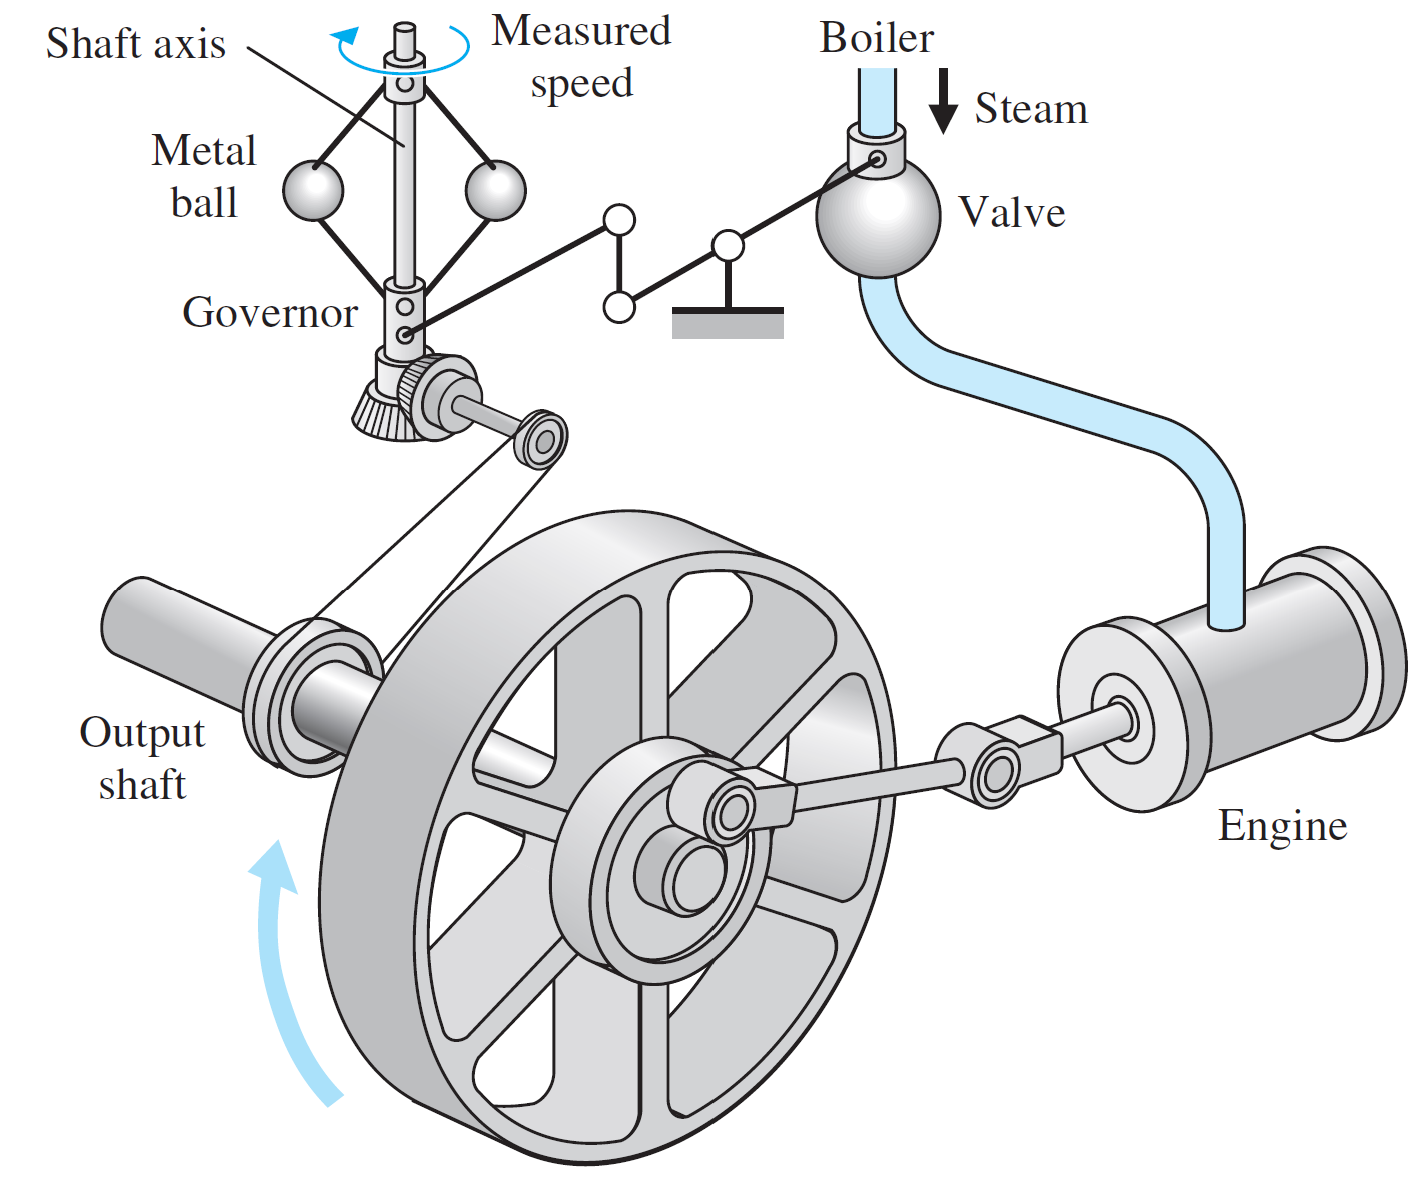
\includegraphics[width=0.75\textwidth]{james-watt-flyball-governer_Dorf-and-Bishop.png}
        \end{column}
        \begin{column}{0.5\textwidth}
            % \footnotesize
            \textbf{How it works}
            \begin{itemize}
                \setlength{\itemsep}{2pt}
                \item Speed rises $\Rightarrow$ balls swing outward
                \item Linkage closes the steam valve
                \item Less steam $\Rightarrow$ engine slows down
            \end{itemize}
            % \vspace{0.4em}
            % \textbf{The loop, in our terms}\\[2pt]
            % \renewcommand{\arraystretch}{1.1}
            % \begin{tabular}{@{}l@{\;\;}l@{}}
            %     \alert{Sensor}      & spinning balls \\
            %     \alert{Controller}  & mechanical linkage \\
            %     \alert{Actuator}    & steam valve \\
            %     \alert{Plant}       & steam engine \\
            %     \alert{Disturbance} & change in load \\
            % \end{tabular}
        \end{column}
    \end{columns}
    \blfootnote{\tiny Image credit: Dorf \& Bishop, \emph{Modern Control Systems}, 2017, 13th ed., Pearson.}
\end{frame}

\begin{frame}
    \centering
    \Large What will you learn in this course? 
\end{frame}

\begin{frame}{What Will You Learn In This Course?}
    % What we will learn in this course:
    % \begin{itemize}
    %     \item How to model a dynamical system (plant) and its components (actuators, sensors, controllers, etc.)
    %     \item How to analyze the system's behavior (stability, transient response, steady-state error, etc.)
    %     \item How to design a controller to achieve desired performance (PID, lead-lag, state feedback, etc.)
    %     \item How to implement the controller in real-time (using microcontrollers etc.)
    %     \item How to test and validate the system's performance (simulation, experiments, etc.)
    % \end{itemize}

    %% adding falling humanoid and exploded rocket images
    By \textbf{midterm}, you will have enough knowledge to prevent your system from blowing up (System Stability).
    \newline
    % \vspace{1em}
    \begin{center}
        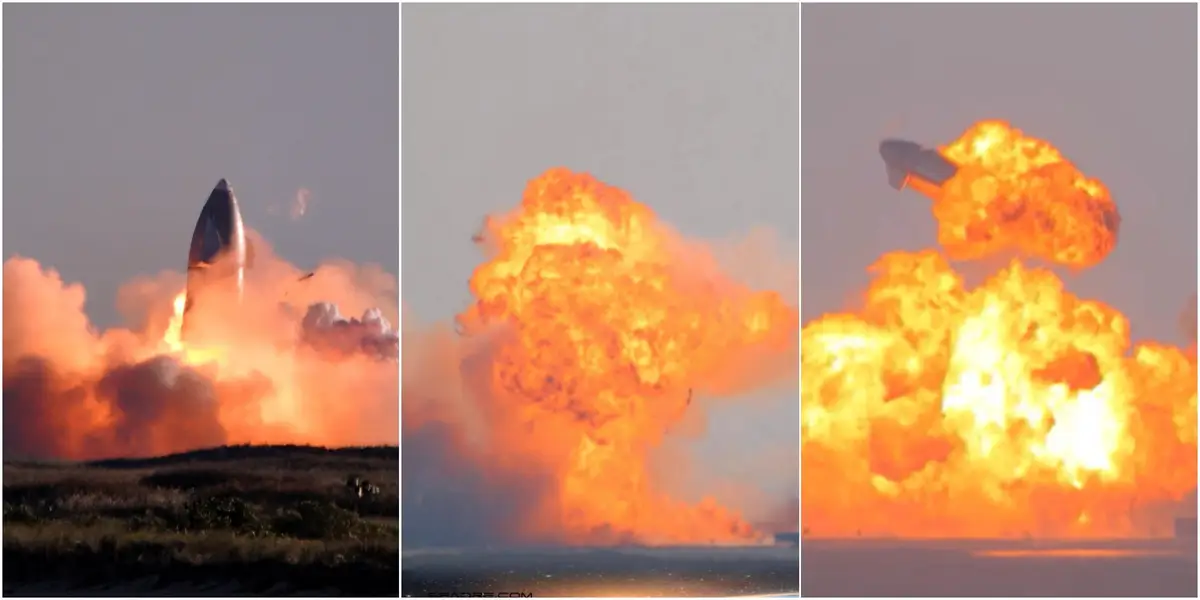
\includegraphics[width=0.6\textwidth]{SpaceX_RocketExplosion.png} 
        \\ Three previous explosions of Starship prototypes\blfootnote{\tiny Gene Blevins/Reuters; SPadre.com}
    \end{center}
\end{frame} 

\begin{frame}{What Will You Learn In This Course?}
    By \textbf{the end of the course}, you will be able to design a controller that makes your system behave as desired (System Performance).
    \newline
    % \vspace{1em}
    \begin{center}
        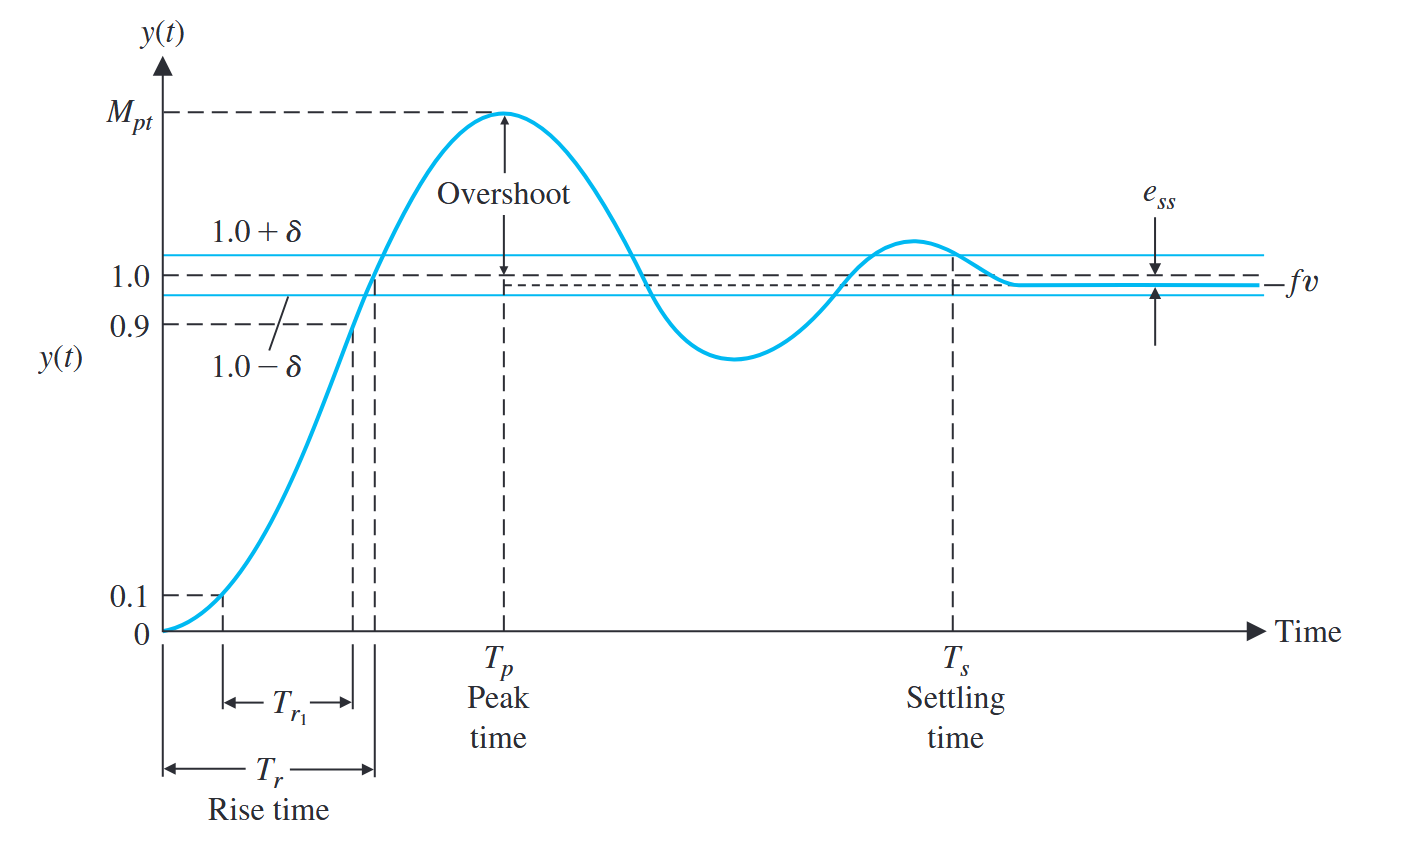
\includegraphics[width=0.5\textwidth]{step_response_of_2nd-order_system_Dorf-Bishop.png}
        \\ Step response of a 2nd-order system and its transient-response specifications\blfootnote{\tiny Image credit: Dorf \& Bishop, \emph{Modern Control Systems}, 2017, 13th ed., Pearson.}
    \end{center}
\end{frame}

\begin{frame}{Course Schedule (1st Semester 2026)}

    \renewcommand{\arraystretch}{1.25}
    \setlength{\tabcolsep}{3pt}
    \tiny
    % \begin{tabular}{@{}p{0.4cm}p{3.5cm}p{5.0cm}p{2.6cm}@{}}
    % สอบกลางภาค
    % 23 ก.ย. 2569 13:00 - 16:00
    % สอบปลายภาค
    % 30 พ.ย. 2569 08:30 - 11:30
    % Homework due 10 days after assigned, unless otherwise specified

    
    \begin{tabular}{r|r|l|l|c|l}
    \hline
    \rowcolor{brandred20}
    \textbf{Wk} & \textbf{Date} & \textbf{Topic} & \textbf{Details} & \textbf{Assignment} &\textbf{Servo Mini-lab (45 mins)} \\
    \hline
    1 & 3 Aug & Intro \& Math Primer & Open-/Closed-Loop Control $\cdot$ ODEs $\cdot$ Laplace & HW1 & \\
    % 1 & 4,6 Aug & Intro \& Math Primer & Open-/Closed-Loop Control $\cdot$ ODEs $\cdot$ LTI $\cdot$ Laplace & HW1 & \\
    % Open/closed loop, anatomy; m-s-d ODE; Laplace; LTI \& convolution; \alert{SS preview} &
    % Laplace Transform; LTI \& Convolution; State Space &
    % \fillin{form teams / kit pickup?} \\
    % \hline
    2 & 10 Aug & Modeling I & LTI $\cdot$ Transfer Functions $\cdot$ Elec./Mech. Systems & & Lab1: Intro \& Setup\\
    % 2 & 11, 13 Aug & System Modeling I & Transfer Functions $\cdot$ Elec./Mech. Systems & & Lab1: Intro \& Setup\\
    % State Space; $A,B,C,D$; $e^{At}$, eigenvalues ue theo
    % \fillin{...} \\
    % \hline
    3 & 17 Aug & Modeling II & State Space $\cdot$ Nonlinearities $\cdot$ Linearization & HW2 & \\
    % 3 & 18, 20 Aug & Sytem Modeling II & State Space $\cdot$ Nonlinearities $\cdot$ Linearization & HW2 & \\
    % % \alert{TF $\leftrightarrow$ SS}, canonical forms; MIMO; DC motor + gears; linearization &
    % % \fillin{motor sys-ID / bench setup?} \\
    % \hline
    4 & 24 Aug & Time Response & 1st/2nd-order $\cdot$ Transient-Response Specifications& HW3 & Lab2: Time Response\\
    % 4 & 25, 27 Aug & Time Response & 1st/2nd-order $\cdot$ Transient-Response Specifications& HW3 & Lab2: Time Response\\
    % % 1st/2nd-order; poles/zeros; $\zeta,\omega_n$; rise / OS / settling &
    % % \fillin{...} \\
    % \hline
    5 & 31 Aug & Block Diagrams & Reduction $\cdot$ Equivalent Forms $\cdot$ Feedback Loop  & &\\
    % 5 & 1, 3 Sep & Block Diagrams & Reduction $\cdot$ Equivalent Forms $\cdot$ Feedback Loop  & &\\
    % % Reduction; closed-loop TF; \alert{SS feedback $A-BK$}; cascade control &
    % % \fillin{...} \\
    % \hline
    6 & 7 Sep & Stability & Routh--Hurwitz Criterion $\cdot$ Gain Range for Stability & HW4 & Lab3: P-Control \& Stability \\
    % 6 & 8, 10 Sep & Stability & Routh--Hurwitz Criterion $\cdot$ Gain Range for Stability & HW4 & Lab3: P-Control \& Stability \\
    % % Routh--Hurwitz; \alert{eig$(A)=$ poles}; $K_p$ range &
    % \alert{Motor setup report due} \\
    % \hline
    7 & 14 Sep & Midterm Review & Cover Topics from Weeks 1--6 & & \\
    % 7 & 15, 17 Sep & Midterm Review & Cover Topics from Weeks 1--6 & & \\
    % Problems first; synthesis second &
    % % \fillin{...} \\
    \midrule
    \multicolumn{6}{l}{Midterm Exam: Wednesday, 23 Sep 2026, 13:00 - 16:00} \\
    \midrule
    % \pause
    8 & 28 Sep & Steady-State Errors & System Type $\cdot$ Gain Design $\cdot$ Disturbances & HW5 & \\
    % 8 & 29 Sep, 1* Oct & Steady-State Errors & System Type $\cdot$ Gain Design $\cdot$ Disturbances & HW5 & \\
    % System type; state aug. $\dot x_e{=}r{-}y$; \alert{integral action; PID} &
    % % \fillin{controller spec/design start?} \\
    % \hline
    9 & 5 Oct & Root Locus I & Rules for Sketching $\cdot$ Transient Response via Gain & HW6 & \\
    % 9 & 6, 8 Oct & Root Locus I & Rules for Sketching $\cdot$ Transient Response via Gain & HW6 & \\
    % The 8 rules; \alert{RL $\equiv$ SS char.\ poly}; sketching &
    % \fillin{...} \\
    % \hline
    10 & 12 Oct & Root Locus II & PI/PD/PID Controller $\cdot$ Lead/Lag Compensation& & Lab4: Root Locus \\
    % 10 & 13*, 15 Oct & Root Locus II & PI/PD/PID Controller $\cdot$ Lead/Lag Compensation& & Lab4: Root Locus \\
    % Lead/lag; PID via RL; \alert{Ziegler--Nichols}; PZC pitfalls &
    % % \fillin{controller design due?} \\
    % \hline
    11 & 19 Oct & Frequency Response I & Asymptotic Bode Plots $\cdot$ Bandwidth & HW7 & \\
    % 11 & 20, 22 Oct & Frequency Response I & Asymptotic Bode Plots $\cdot$ Bandwidth & HW7 & \\
    % Asymptotic Bode; construction; \alert{SS frequency response} &
    % \fillin{...} \\
    % \hline
    12 & 26 Oct & Frequency Response II & Nyquist \& Stability Margins $\cdot$ Lead/Lag $\cdot$ PI/PD/PID & &  Lab5: Frequency Response\\
    % 12 & 27, 29 Oct & Frequency Response II & Nyquist \& Stability Margins $\cdot$ Lead/Lag $\cdot$ PI/PD/PID & &  Lab5: Frequency Response\\
    % Nyquist; gain/phase margins; sensitivity $S$, $T$ &
    % % \fillin{implementation / HIL?} \\
    % \hline
    13 & 2 Nov & Design via State Space & Controllability $\cdot$ Full-State Feedback (Pole Placement) & HW8 & Lab6: Pole Placement\\
    % 13 & 3, 5 Nov & Design via State Space & Controllability $\cdot$ Full-State Feedback (Pole Placement) & HW8 & Lab6: Pole Placement\\
    % Controllability \& observability; \alert{pole placement, Ackermann}; observer &
    % % \fillin{dry-run / checkoff?} \\
    % \hline
    14 & 9 Nov & Project Demo Day & Group Presentations & \\
    % 14 & 10, 12 Nov & Project Demo Day & Group Presentations $\cdot$ Control Competition & \\
    % Diagnostic-fix presentations; tracking competition; judging &
    % % \alert{Demo + competition} \\
    % \hline
    15 & 16 Nov & Final Review & Cover ALL Topics& \\
    % 15 & 17, 19 Nov & Final Review & Cover ALL Topics& \\
    % Recap W8--13; common pitfalls; exam strategy &
    % % \fillin{final report due?} \\
    % % \hline
    \midrule
    \multicolumn{5}{l}{Final Exam: Monday, 30 Nov 2026, 8:30 - 11:30} \\
    \midrule
    \multicolumn{6}{r}{\textbullet~\textit{Homework is due \textbf{ten days} after it is assigned unless otherwise specified.}} \\
    \multicolumn{6}{r}{\textbullet~\textit{Pre-lab handout released \textbf{one week} before each mini-lab; reading required before the session.}} \\
    \multicolumn{6}{r}{\textbullet~\textit{Lab Report (4 people per group) is due \textbf{one week} after the lab session.}} \\
    \end{tabular} 
\end{frame}

\begin{frame}{Servo Mini-Lab (10\% of the grade)}
    \begin{columns}

        \begin{column}{0.6\textwidth}
            \begin{itemize}
                \item 45-minute hands-on sessions with a brushed DC motor system
                % \item Learn how to model a dynamical system (plant) and its components (actuators, sensors, controllers, etc.)
                % \item Implement your controller on a real-time hardware setup (Brushed DC motor system)
                \item Learn how to use MATLAB/Simulink to model, analyze, and design control systems on a real-time hardware setup
                % \item Lab reports are due one week after the lab session
                \item \alert{Must Bring} at least one laptop (+ USB-C data cable) per group with MATLAB/Simulink and required toolboxes installed
                \item \textbf{Note:} Lab sessions are mandatory and will be graded
            \end{itemize}
        \end{column}

        \begin{column}{0.4\textwidth}
            \includegraphics[width=0.75\textwidth]{graphic_files/minilab_dc_motor_plant.png}
        \end{column}
    \end{columns}
\end{frame}

\begin{frame}{Final Project (15\% of the grade)}
    Groups of 4, starting after the midterm. 
    \vspace{0.5em}
    \begin{columns}[c]
        \begin{column}{0.62\textwidth}
            You will be given an electro-mechanical plant and must make it meet a target
            performance specification:
            \begin{itemize}
                \item \alert{Identify} the plant model from experiment
                \item \alert{Simulate} it in Simulink and validate against hardware
                \item \alert{Design and tune} a controller to meet the specification
                \item \alert{Demonstrate} it on the real plant, and explain any
                      simulation-vs-hardware mismatch
            \end{itemize}
        \end{column}
        \begin{column}{0.38\textwidth}
            \centering
            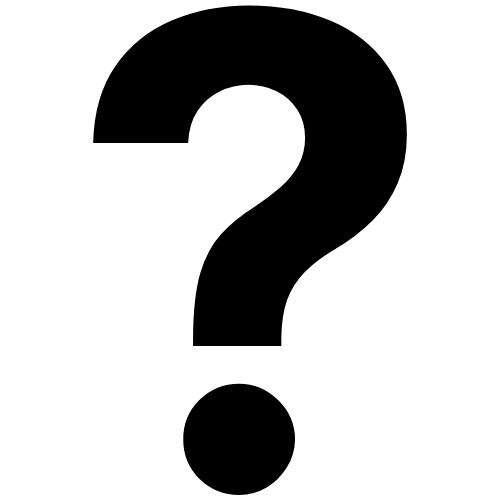
\includegraphics[height=3.2cm, keepaspectratio]{Black_question_mark.png}\\[4pt]
            {\small Plant: to be announced}
        \end{column}
    \end{columns}
    % \vspace{0.6em}
    % \begin{center}
    %     \scriptsize
    %     \textbf{Wk 9} System ID $\;\rightarrow\;$
    %     \textbf{Wk 11} Design in simulation $\;\rightarrow\;$
    %     \textbf{Wk 13} Hardware tuning $\;\rightarrow\;$
    %     \textbf{Wk 14} Demo day \& report
    % \end{center}
\end{frame}

\begin{frame}{}
    \begin{columns}
        \begin{column}{0.15\textwidth}
        The Bigger Picture... \newline \newline
        How much of this do you think we cover?
        \end{column}
        \begin{column}{0.85\textwidth}
            \centering
            \only<1>{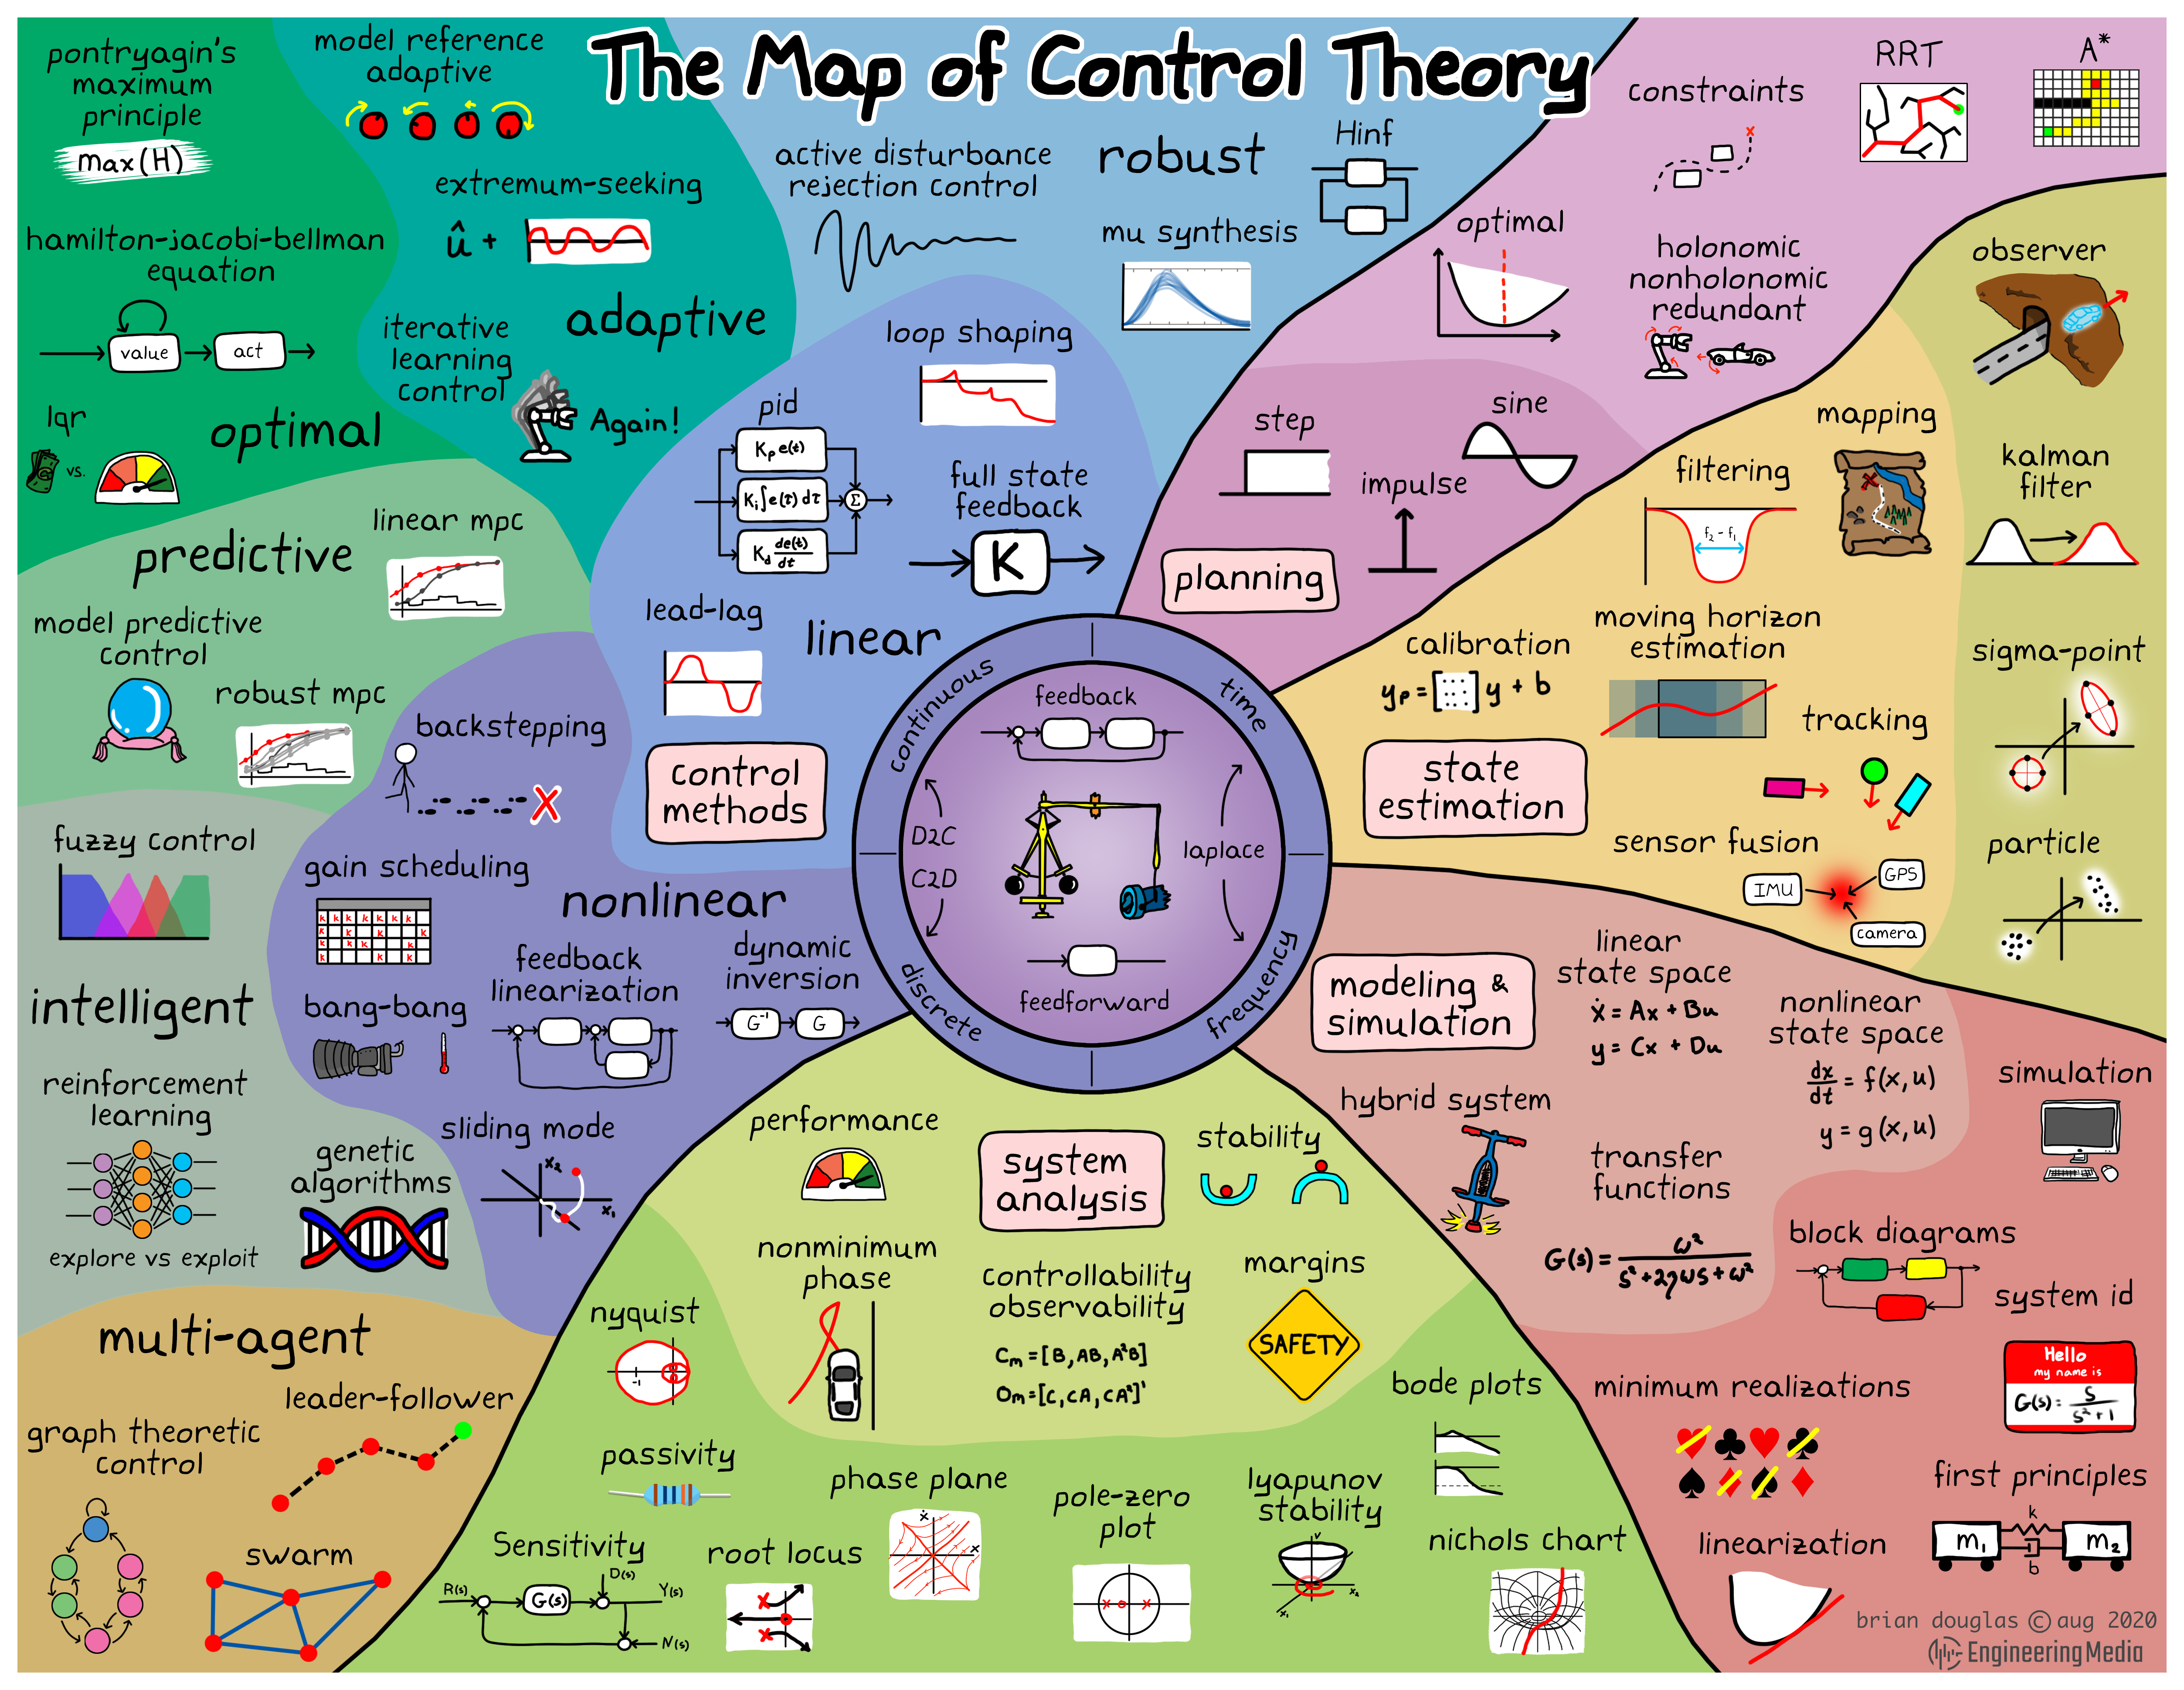
\includegraphics[width=0.9\textwidth]{Control_Map_ver5.png}}%
            \only<2>{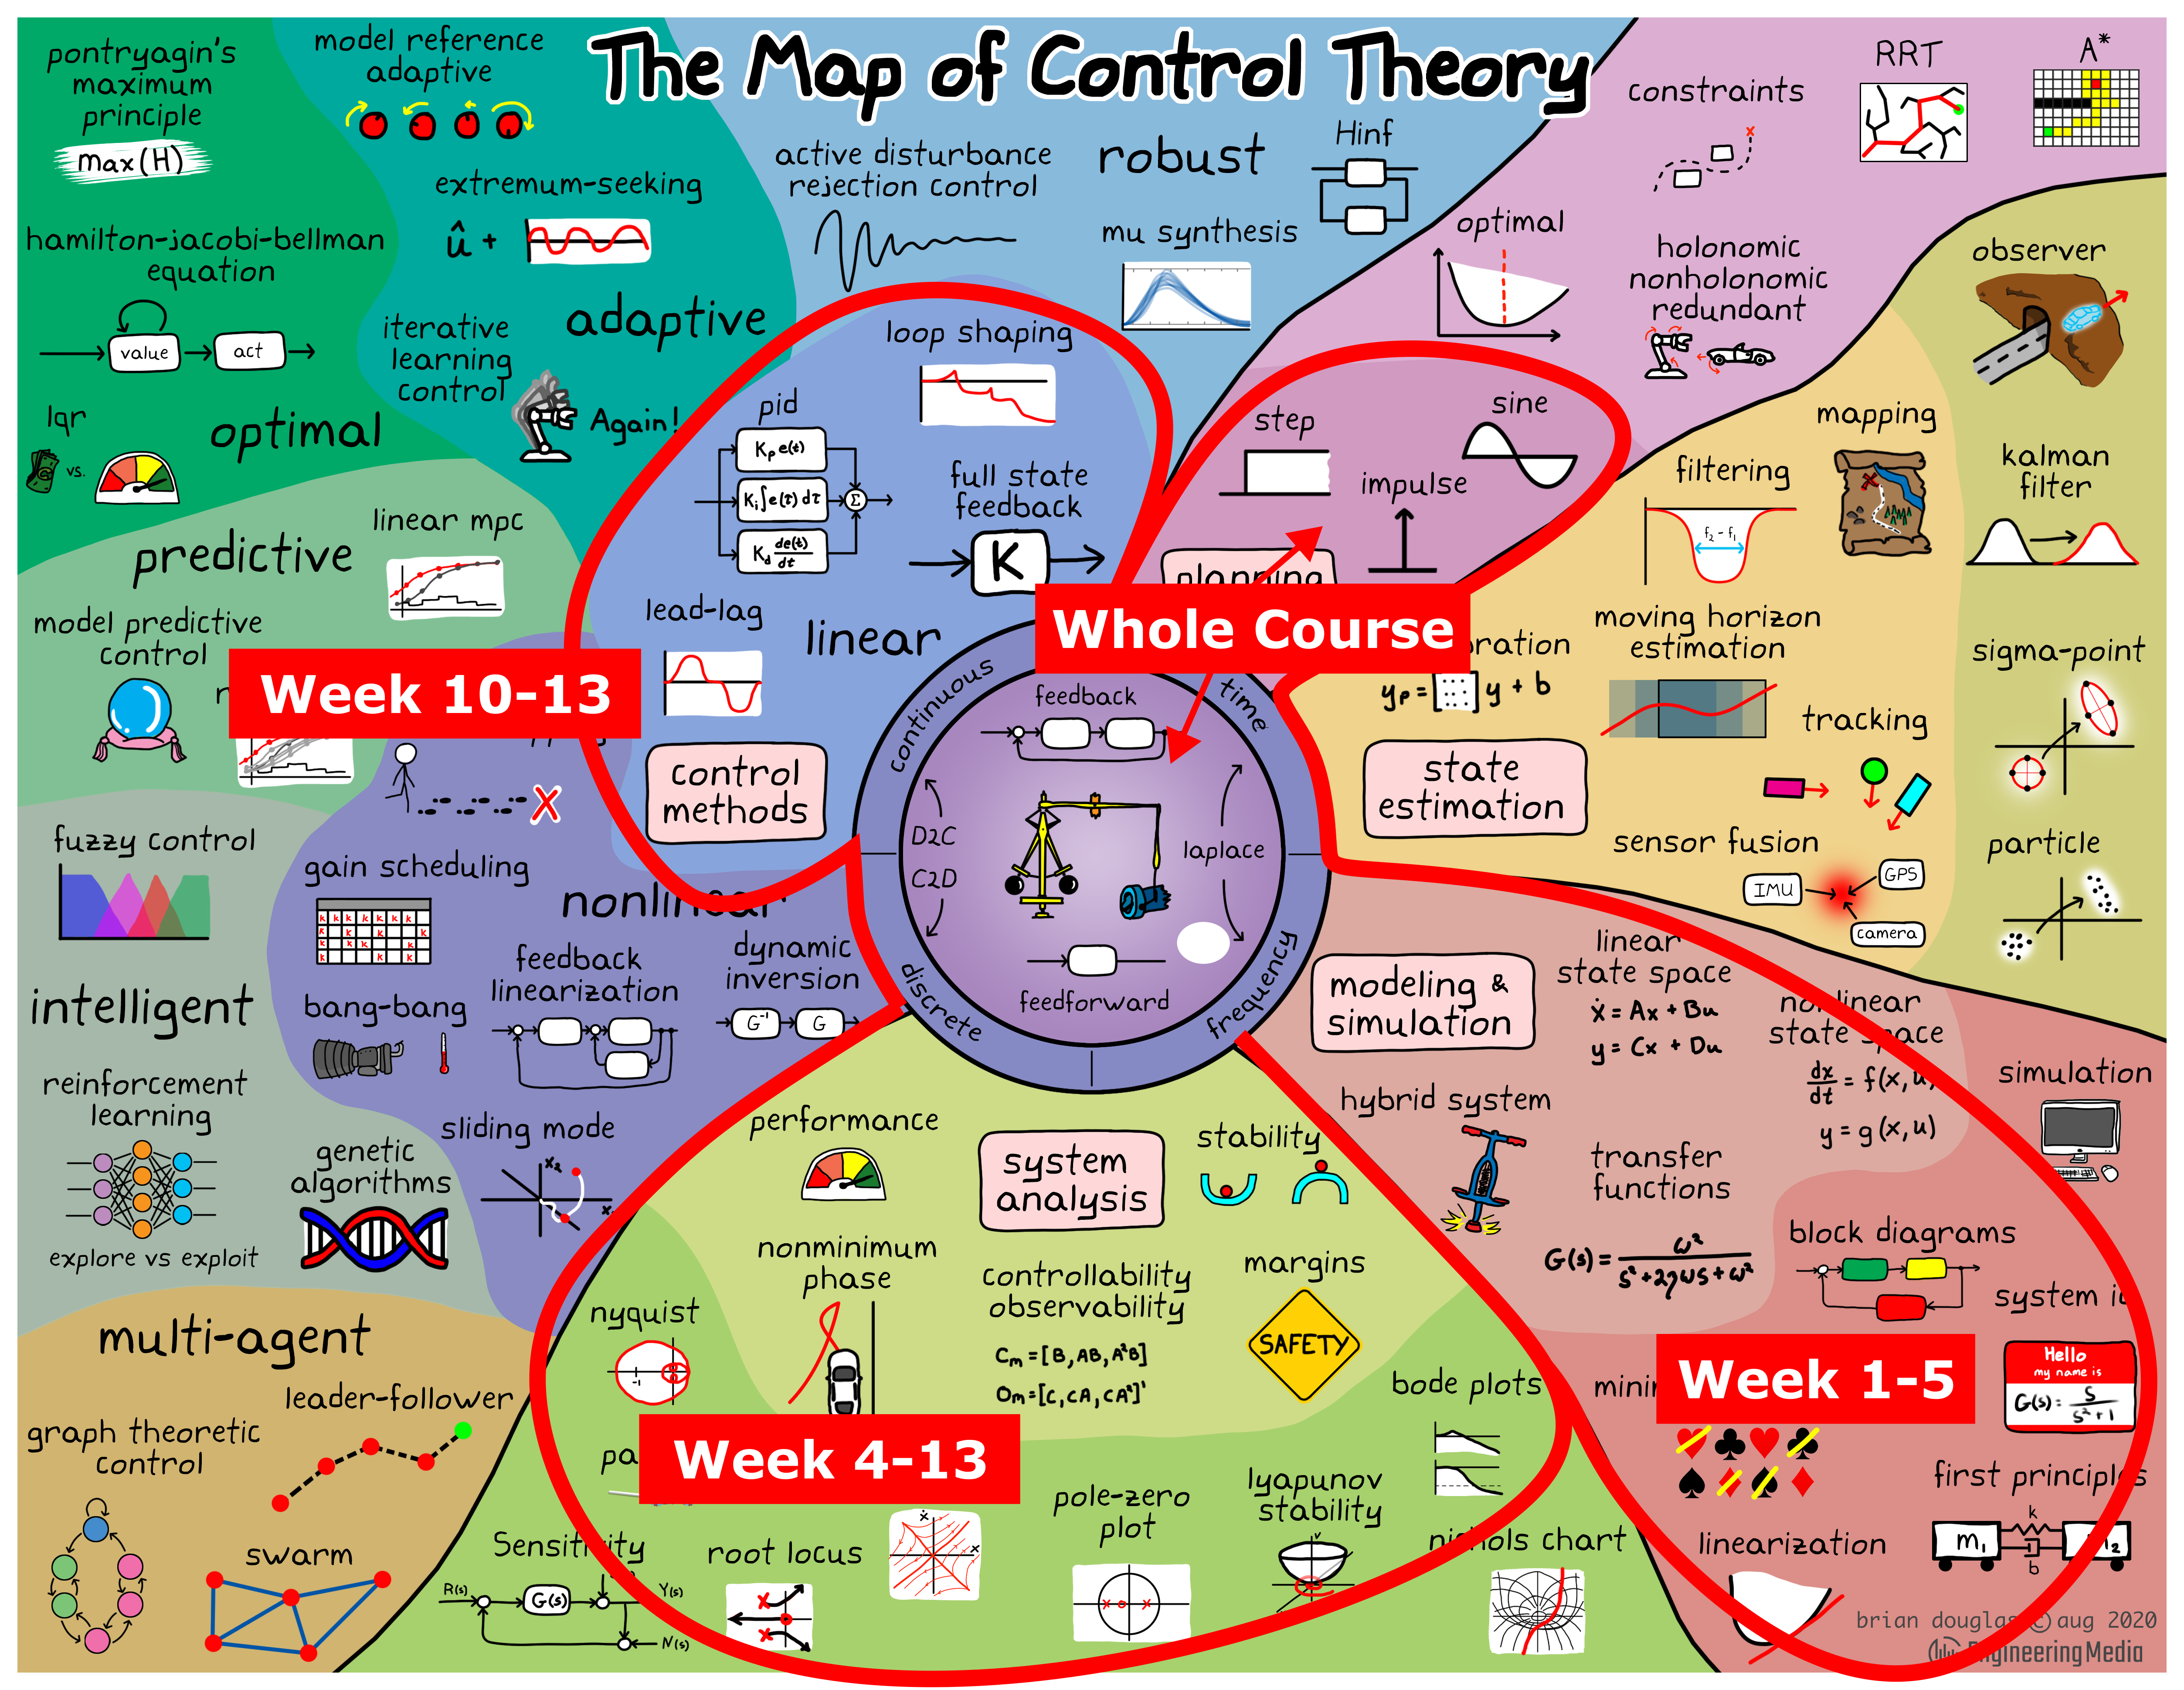
\includegraphics[width=0.9\textwidth]{Control_Map_Annotated.png}}%
            \\ \tiny (Image Credit: Brian Douglas)
        \end{column}
    \end{columns}
\end{frame}
\section{Dynamic System Modeling, ODEs, and Laplace Transform}

\begin{frame}{How Do We Model Each Block?}
    A control system is a set of interconnected subsystems. To design anything, we first
    need a model of each one.
    \begin{center}
        \begin{tikzpicture}[
            auto, >=latex',
            scale=0.95, transform shape,
            block/.style={draw, rectangle, minimum height=2.9em, minimum width=6.8em, align=center},
            input/.style={coordinate},
            output/.style={coordinate},
        ]
            \node [block, draw=brandred, text=brandred, very thick] (plant) at (0,0)
                {Subsystem\\[1pt] \small (plant, actuator, sensor, \dots)};
            \node [input]  (in)  at (-5.2,0) {};
            \node [output] (out) at ( 5.2,0) {};
            \draw [->, black, very thick] (in) -- node [above] {input $u$} (plant);
            \draw [->, black, very thick] (plant) -- node [above] {output $y$} (out);
        \end{tikzpicture}
    \end{center}
    \begin{itemize}
        \item Every block is described the same way: by its
              \alert{input--output relationship}.
        \item That relationship is governed by a \alert{differential equation}
              in the time domain %, or a \alert{transfer function} in the $s$-domain.
        \item Next: how to compute the output $y(t)$ given an input $u(t)$ and a differential equation.
    \end{itemize}
\end{frame}

\begin{frame}{Dynamic System Modeling}
    \begin{center}
        Consider the linear mass--spring--damper system below,\newline 
        \massSpringDamper[1.0] 
    \end{center}
    with mass $m = \SI{1}{kg}$, damping $c = \SI{2}{N.s/m}$, and stiffness $k = \SI{3}{N/m}$.\newline
    Here $f(t)$ is the applied force (input) and $x(t)$ is the displacement from equilibrium (output). All surfaces are smooth and frictionless.
\end{frame}

\begin{frame}{Solving ODEs in Time Domain}
    \begin{columns}
        \begin{column}{0.5\columnwidth}
            \centering
            \massSpringDamper[0.75] 
        \end{column}
        \begin{column}{0.5\columnwidth}
            \centering
            \begin{tikzpicture}
                \begin{axis}[
                    % Force markers to draw on top of grids/axis lines
                    set layers, mark layer=axis foreground,
                    width=\linewidth, height=3cm,
                    xlabel={$t$}, ylabel={$f(t)$},
                    xmin=0, xmax=4, ymin=-120, ymax=120,
                    xtick={0,1,2,3}, ytick={-100,-50,0,50,100},
                    axis lines=left,
                    % axis lines=center,
                    every axis x label/.style={at={(current axis.right of origin)},anchor=north west},
                    every axis y label/.style={at={(current axis.above origin)},anchor=south east},
                    clip=false,
                ]
                    % input f(t) = 100 sin(2 pi t)
                    \addplot[very thick, red, smooth, samples=400, domain=0:4]{100*sin(deg(2*pi*x))};
                \end{axis}
            \end{tikzpicture}
        \end{column}
    \end{columns}
    \vspace{1em}
    From Newton's second law, the governing Ordinary Differential Equation (ODE) is
    \[
        m \ddot{x}(t) + c\dot{x}(t) + kx(t) = f(t), 
    \] or with the given parameters, it becomes
    \[
        \ddot{x}(t) + 2\dot{x}(t) + 3x(t) = f(t), 
    \]
    Given the input force $f(t) = 100\,\sin(2\pi t)\,\text{N}$ , with all zero initial conditions $(x(0) = 0 \text{m}, \dot{x}(0) = 0 \text{m/s})$, solve the ODE to find the output $x(t)$.
    % particular solution, homogeneous solution, and general solution 
\end{frame}

\begin{frame}{Solving ODEs in Time Domain: The Procedure}
    For a linear ODE, the total solution is the sum of two parts:
    \[
        x(t) \;=\; \underbrace{x_h(t)}_{\text{homogeneous}} \;+\; \underbrace{x_p(t)}_{\text{particular}}
    \]
    \begin{enumerate}
        \item \alert{Homogeneous solution} $x_h$: solve the ODE with $f(t) = 0$.
              Its shape is set by the \emph{system} (contains the unknown constants).
        \item \alert{Particular solution} $x_p$: find any one solution of the full ODE
              with $f(t)$. Its shape is set by the \emph{input}.
        \item Add them, then apply the \alert{initial conditions} to determine the
              remaining constants.
    \end{enumerate}
    \vspace{0.3em}
    \begin{center}
        \alert{Careful:} the initial conditions apply to $x_h + x_p$, never to $x_h$ alone.
    \end{center}
\end{frame}

\begin{frame}{Step 1: Homogeneous Solution (Transient)}
    Set $f(t) = 0$ and try $x = e^{st}$:
    \[
        \ddot{x} + 2\dot{x} + 3x = 0
        \;\;\Longrightarrow\;\;
        \underbrace{(s^2 + 2s + 3)}_{\text{characteristic polynomial}} e^{st} = 0
    \]
    The exponential is never zero, so the \alert{characteristic equation} must hold:
    \[
        s^2 + 2s + 3 = 0 \;\;\Longrightarrow\;\; s = -1 \pm j\sqrt{2}
    \]
    Complex roots with a negative real part: the system is \alert{underdamped} and stable.
    \[
        x_h(t) = e^{-t}\left(A\cos\sqrt{2}\,t + B\sin\sqrt{2}\,t\right)
    \]
    \begin{itemize}
        \item Real part $-1$: decay rate. Imaginary part $\sqrt{2}$: damped frequency.
        \item $A$ and $B$ are still unknown, and $x_h \to 0$: this is the \alert{transient}.
    \end{itemize}
\end{frame}

\begin{frame}{Step 2: Particular Solution (Steady State)}
    The input is a sinusoid at $\omega = 2\pi$ rad/s, so try the same form
    (\alert{method of undetermined coefficients}):
    \[
        x_p(t) = C\cos\omega t + D\sin\omega t
    \]
    Substituting into $\ddot{x} + 2\dot{x} + 3x = 100\sin\omega t$ and matching the
    $\cos\omega t$ and $\sin\omega t$ terms:
    \[
        \begin{array}{rcl}
            (3-\omega^2)\,C + 2\omega\,D &=& 0\\[2pt]
            -2\omega\,C + (3-\omega^2)\,D &=& 100
        \end{array}
        \qquad
        \begin{array}{l}
            3-\omega^2 = -36.48\\[2pt]
            2\omega = 12.57
        \end{array}
    \]
    \[
        \Longrightarrow\quad C = -0.844, \quad D = -2.451
        \qquad
        x_p(t) = 2.59\,\sin(2\pi t - 161^\circ)
    \]
    \begin{itemize}
        \item Amplitude $=\dfrac{100}{\sqrt{(3-\omega^2)^2 + (2\omega)^2}} = 2.59$ m:
              the same frequency as the input, but scaled and phase-shifted.
        \item $x_p$ never decays: this is the \alert{steady-state} response.
    \end{itemize}
\end{frame}

\begin{frame}{Step 3: Apply the Initial Conditions}
    \[
        x(t) = e^{-t}\left(A\cos\sqrt{2}\,t + B\sin\sqrt{2}\,t\right)
               - 0.844\cos 2\pi t - 2.451\sin 2\pi t
    \]
    With $x(0) = 0$ and $\dot{x}(0) = 0$: \quad $A = 0.844$, \quad $B = 11.48$.
    \begin{columns}[c]
        \begin{column}{0.56\textwidth}
            \centering
            \begin{tikzpicture}
                \begin{axis}[
                    width=\linewidth, height=4cm,
                    xlabel={$t$ (s)}, ylabel={$x(t)$ (m)},
                    xmin=0, xmax=6, ymin=-13, ymax=13,
                    xtick={0,1,2,3,4,5,6}, ytick={-10,0,10},
                    axis lines=left,
                    every axis x label/.style={at={(current axis.right of origin)},anchor=north west},
                    every axis y label/.style={at={(current axis.above origin)},anchor=south east},
                    clip=false,
                ]
                    \addplot[thick, black, dashed, smooth, samples=500, domain=0:6]
                        {-0.8442*cos(deg(2*pi*x)) - 2.4505*sin(deg(2*pi*x))};
                    \addplot[very thick, blue, smooth, samples=600, domain=0:6]
                        {exp(-x)*(0.8442*cos(deg(sqrt(2)*x)) + 11.4844*sin(deg(sqrt(2)*x)))
                         - 0.8442*cos(deg(2*pi*x)) - 2.4505*sin(deg(2*pi*x))};
                \end{axis}
            \end{tikzpicture}
        \end{column}
        \begin{column}{0.42\textwidth}
            \small
            \textcolor{blue}{\rule{1em}{1.2pt}} total response $x(t)$\\[3pt]
            \textcolor{black}{\rule{1em}{0.8pt}} steady state $x_p(t)$
            \begin{itemize}
                \item The transient dominates early, then dies out with time
                      constant $1/1 = 1$ s.
                \item After $\approx 4$--$5$ s only $x_p$ remains.
            \end{itemize}
        \end{column}
    \end{columns}
\end{frame}

%%%%%%%%%%%%%%%%%%%%%%%%%%%%%%%%%%%%%%%%%%%%%%%%%%%%%%%%%%%%%%%%%%%%%%%%%%%%%%%%%

\begin{frame}{Non-continuous Forcing Function}
    \begin{columns}
        \begin{column}{0.5\textwidth}
            How do we solve ODEs if the forcing function is a square pulse like this?
            % \[
            %     u(t-1) - u(t-2)
            % \]
            % \begin{itemize}
            %     \item $u(t-1)$ turns \emph{on} at $t = 1$
            %     \item $-u(t-2)$ turns it back \emph{off} at $t = 2$
            % \end{itemize}
        \end{column}
        \begin{column}{0.5\textwidth}
            \centering
            \begin{tikzpicture}
                \begin{axis}[
                    % Force markers to draw on top of grids/axis lines
                    set layers, mark layer=axis foreground,
                    width=\linewidth, height=5cm,
                    xlabel={$t$}, ylabel={$f(t)$},
                    xmin=0, xmax=3.5, ymin=-0.3, ymax=1.4,
                    xtick={0,1,2,3}, ytick={0,1},
                    axis lines=left,
                    every axis x label/.style={at={(current axis.right of origin)},anchor=north west},
                    every axis y label/.style={at={(current axis.above origin)},anchor=south east},
                    clip=false,
                ]
                    % rectangular pulse u(t-1)-u(t-2)
                    \addplot[very thick, red, const plot mark left] coordinates {
                        (0,0) (1,0) (1,1) (2,1) (2,0) (3.5,0)
                    };
                    % open/closed circles at the jumps
                    % \addplot[only marks, mark=*, blue] coordinates {(1,1) (2,0)};
                    % \addplot[only marks, mark=o, blue, fill=white] coordinates {(1,0) (2,1)};
                    % \node[blue, anchor=north] at (axis cs:1.5,1) {\small $u(t-1)-u(t-2)$};
                \end{axis}
            \end{tikzpicture}
        \end{column}
    \end{columns}
\end{frame}

%%%%%%%%%%%%%%%%%%%%%%%%%%%%%%%%%%%%%%%%%%%%%%%%%%%%%%%%%%%%%%%%%%%%%%%%%%%%%%%%%

\begin{frame}{Dirac Delta Function}
    The \emph{Dirac delta function} $\delta(t)$, also known as the ``unit'' impulse function.
    \vspace{1em}
    \begin{columns}
        \begin{column}{0.5\textwidth}
                It is an \emph{infinitely} tall, \emph{infinitesimally} narrow spike whose area is exactly one,
            \[
                \delta(t) =
                \begin{cases}
                    \infty, & t = 0 \\
                    0,      & t \neq 0
                \end{cases}
            \]
            such that
                \[
                    \int_{-\infty}^{\infty}\!\! \delta(t)\,dt = 1.
                \]
        \end{column}
        \begin{column}{0.5\textwidth}
            \centering
\begin{tikzpicture}
    \begin{axis}[
        % Force markers to draw on top of grids/axis lines
        set layers, mark layer=axis foreground,
        width=\linewidth, height=5cm,
        xlabel={$t$}, ylabel={$\delta(t)$},
        xmin=-0.25, xmax=0.25, ymin=-0.25, ymax=1.25,
        xtick={0}, ytick={1}, yticklabels={$1$},
        axis lines=center,
        every axis x label/.style={at={(current axis.right of origin)},anchor=south west},
        every axis y label/.style={at={(current axis.above origin)},anchor=south},
        clip=false,
    ]
        % arrow of "unit area" at t=0 (standard impulse convention)
        \addplot[very thick, red, -{Stealth[length=3mm]}] coordinates {(0,0) (0,1)};
        % baseline
        \addplot[very thick, red] coordinates {(-0.15,0) (0.15,0)};
        % \addplot[only marks, mark=o, red, fill=white] coordinates {(0,0)};
        \node[red, anchor=south west] at (axis cs:0.05,0.95) {\small (area $=1$)};
    \end{axis}
\end{tikzpicture}
        \end{column}
    \end{columns}
    \vspace{1em}
    It is the basic building block for constructing any input signal. So how does a system response to it?
\end{frame}

%%%%%%%%%%%%%%%%%%%%%%%%%%%%%%%%%%%%%%%%%%%%%%%%%%%%%%%%%%%%%%%%%%%%%%%%%%%%%%%%%

\begin{frame}{Unit Impulse Response}
    \begin{columns}
        \begin{column}{0.5\textwidth}
            \begin{center}
                \massSpringDamper[0.7]
            \end{center}
            Strike the system with a \textcolor{red}{unit impulse $\delta(t)$}, a sharp ``hammer blow.''
            \newline \newline
            The output \textcolor{blue}{$h(t)$} is the \textcolor{blue}{\emph{unit impulse response}}: a signature of the system's natural behavior.
            % \[
            %     h(t) = \frac{1}{\sqrt{2}}\,e^{-t}\sin\!\left(\sqrt{2}\,t\right).
            % \]
        \end{column}
        \begin{column}{0.5\textwidth}
            \centering
            \begin{tikzpicture}
                \begin{groupplot}[
                    group style={
                        group size=1 by 2,
                        vertical sep=35pt,
                        % xticklabels at=all,
                        x descriptions at=all, 
                    },
                    width=\linewidth, height=3.2cm,
                    xmin=0, xmax=8,
                    ticks=none,
                    xlabel={$t$},
                    axis lines=center,
                    axis line style={-{Stealth[length=2mm]}},
                    every axis x label/.style={at={(current axis.right of origin)},anchor=north west},
                    every axis y label/.style={at={(current axis.above origin)},anchor=south},
                    clip=false,
                ]
                    % top: input -- unit impulse delta(t)
                    \nextgroupplot[ylabel={$f(t)$}, ymin=0, ymax=1.4]
                        % \addplot[gray, opacity=0.5, thick, domain=0:8] {0};
                        \addplot[very thick, red, -{Stealth[length=2.5mm]}] coordinates {(0,0) (0,1)};
                        % \node[brandred, anchor=south west] at (axis cs:0.15,0.9) {\small (area $=1$)};
                        \node[red, anchor=west] at (axis cs:0.2,1.0) {\small $\delta(t)$};
                    % bottom: output -- impulse response h(t)
                    \nextgroupplot[ylabel={$x(t)$}, ymin=0, ymax=0.6]
                        % \addplot[gray, opacity=0.5, thick, domain=0:8] {0};
                        \addplot[very thick, blue, smooth, samples=200, domain=0:8]
                            {1/sqrt(2) * exp(-x) * sin(deg(sqrt(2)*x))};
                        \node[blue, anchor=south west] at (axis cs:0.4,0.3) {\small $h(t)$};
                \end{groupplot}
            \end{tikzpicture}
        \end{column}
    \end{columns}
\end{frame}

%%%%%%%%%%%%%%%%%%%%%%%%%%%%%%%%%%%%%%%%%%%%%%%%%%%%%%%%%%%%%%%%%%%%%%%%%%%%%%%%%

\begin{frame}{Unit Impulse Response}
    \begin{columns}[c]
        % --- input: unit impulse delta(t) ---
        \begin{column}{0.33\textwidth}
            \centering
            \begin{tikzpicture}
                \begin{axis}[
                    width=\linewidth, height=3.2cm,
                    xmin=0, xmax=8, ymin=0, ymax=1.4,
                    ticks=none,
                    xlabel={$t$}, ylabel={$f(t)$},
                    axis lines=center,
                    axis line style={-{Stealth[length=2mm]}},
                    every axis x label/.style={at={(current axis.right of origin)},anchor=north west},
                    every axis y label/.style={at={(current axis.above origin)},anchor=south},
                    clip=false,
                ]
                    \addplot[very thick, red, -{Stealth[length=2.5mm]}] coordinates {(0,0) (0,1)};
                    \node[red, anchor=west] at (axis cs:0.2,1.0) {\small $\delta(t)$};
                \end{axis}
            \end{tikzpicture}
        \end{column}
        % --- block diagram ---
        \begin{column}{0.33\textwidth}
            % \massSpringDamper[0.5] \newline
            \ioDiagram[$f(t)$][System][$x(t)$][0.9]
        \end{column}
        % --- output: impulse response h(t) ---
        \begin{column}{0.33\textwidth}
            \centering
            \begin{tikzpicture}
                \begin{axis}[
                    width=\linewidth, height=3.2cm,
                    xmin=0, xmax=8, ymin=0, ymax=0.6,
                    ticks=none,
                    xlabel={$t$}, ylabel={$x(t)$},
                    axis lines=center,
                    axis line style={-{Stealth[length=2mm]}},
                    every axis x label/.style={at={(current axis.right of origin)},anchor=north west},
                    every axis y label/.style={at={(current axis.above origin)},anchor=south},
                    clip=false,
                ]
                    \addplot[very thick, blue, smooth, samples=200, domain=0:8]
                        {1/sqrt(2) * exp(-x) * sin(deg(sqrt(2)*x))};
                    \node[blue, anchor=south west] at (axis cs:0.9,0.24) {\small $h(t)$};
                \end{axis}
            \end{tikzpicture}
        \end{column}
    \end{columns}
    \centering 
    \vspace{1em}
    The \textcolor{red}{impulse $\delta(t)$} acts only at $t=0$, yet the system keeps responding for $t>0$. \newline
    The \textcolor{blue}{unit impulse response $h(t)$} captures how the system responds after the impulse and settles back to equilibrium.
\end{frame}

%%%%%%%%%%%%%%%%%%%%%%%%%%%%%%%%%%%%%%%%%%%%%%%%%%%%%%%%%%%%%%%%%%%%%%%%%%%%%%%%%

\begin{frame}{Linear System: Homogeneity (Scaling)}
    \begin{columns}[c]
        % --- input: unit impulse delta(t) ---
        \begin{column}{0.33\textwidth}
            \centering
            \begin{tikzpicture}
                \begin{axis}[
                    width=\linewidth, height=3.6cm,
                    xmin=0, xmax=8, ymin=-1.0, ymax=1.3,
                    ticks=none,
                    xlabel={$t$}, ylabel={$f(t)$},
                    axis lines=center,
                    axis line style={-{Stealth[length=2mm]}},
                    every axis x label/.style={at={(current axis.right of origin)},anchor=north west},
                    every axis y label/.style={at={(current axis.above origin)},anchor=south},
                    clip=false,
                ]
                    \addplot[very thick, red, -{Stealth[length=2.5mm]}] coordinates {(0,0) (0,1)};
                    \addplot[very thick, brandred, -{Stealth[length=2.5mm]}] coordinates {(0,0) (0,0.5)};
                    \addplot[very thick, brown, -{Stealth[length=2.5mm]}] coordinates {(0,0) (0,-0.75)};
                    \node[red, anchor=west] at (axis cs:0.2,1.0) {\small $\delta(t)$};
                    \node[brandred, anchor=west] at (axis cs:0.2,0.5) {\small $0.5\,\delta(t)$};
                    \node[brown, anchor=west] at (axis cs:0.2,-0.75) {\small $-0.75\,\delta(t)$};
                \end{axis}
            \end{tikzpicture}
        \end{column}
        % --- block diagram ---
        \begin{column}{0.33\textwidth}
            % \massSpringDamper[0.5] \newline
            \ioDiagram[$f(t)$][\shortstack{Linear\\System}][$x(t)$][0.9]
        \end{column}
        % --- output: impulse response h(t) ---
        \begin{column}{0.33\textwidth}
            \centering
            \begin{tikzpicture}
                \begin{axis}[
                    width=\linewidth, height=3.6cm,
                    xmin=0, xmax=8, ymin=-0.35, ymax=0.45,
                    ticks=none,
                    xlabel={$t$}, ylabel={$x(t)$},
                    axis lines=center,
                    axis line style={-{Stealth[length=2mm]}},
                    every axis x label/.style={at={(current axis.right of origin)},anchor=north west},
                    every axis y label/.style={at={(current axis.above origin)},anchor=south},
                    clip=false,
                ]
                    \addplot[very thick, red, smooth, samples=200, domain=0:8]
                        {1/sqrt(2) * exp(-x) * sin(deg(sqrt(2)*x))};
                    \addplot[very thick, brandred, smooth, samples=200, domain=0:8]
                        {0.5/sqrt(2) * exp(-x) * sin(deg(sqrt(2)*(x)))};
                    \addplot[very thick, brown, smooth, samples=200, domain=0:8]
                        {-0.75/sqrt(2) * exp(-x) * sin(deg(sqrt(2)*(x)))};
                    \node[red, anchor=south west] at (axis cs:0.9,0.24) {\small $h(t)$};
                    \node[brandred, anchor=south west] at (axis cs:2.0,0.05) {\small $0.5\,h(t)$};
                    \node[brown, anchor=north west] at (axis cs:0.9,-0.20) {\small $-0.75\,h(t)$};
                \end{axis}
            \end{tikzpicture}
        \end{column}
    \end{columns}
    % \centering 
    \vspace{1em}
    \alert{\emph{Homogeneity (Scaling):}} multiplying the input by any constant $a$ multiplies the output by the same $a$.
    So each scaled impulse $\delta(t)$ yields an identically scaled impulse response $h(t)$:
    \[
        f(t) = a\,\delta(t) \;\longrightarrow\; x(t) = a\,h(t).
    \]
\end{frame}

%%%%%%%%%%%%%%%%%%%%%%%%%%%%%%%%%%%%%%%%%%%%%%%%%%%%%%%%%%%%%%%%%%%%%%%%

\begin{frame}{Linear System: Additivity}
    \begin{columns}[c]
        % --- input: three inputs and their sum ---
        \begin{column}{0.33\textwidth}
            \centering
            \begin{tikzpicture}
                \begin{axis}[
                    width=\linewidth, height=3.6cm,
                    xmin=0, xmax=8, ymin=-1.0, ymax=1.3,
                    ticks=none,
                    xlabel={$t$}, ylabel={$f(t)$},
                    axis lines=center,
                    axis line style={-{Stealth[length=2mm]}},
                    every axis x label/.style={at={(current axis.right of origin)},anchor=north west},
                    every axis y label/.style={at={(current axis.above origin)},anchor=south},
                    clip=false,
                ]
                    % individual inputs (faded)
                    \addplot[very thick, red,      opacity=0.3, -{Stealth[length=2.5mm]}] coordinates {(0,0) (0,1)};
                    \addplot[very thick, brandred, opacity=0.3, -{Stealth[length=2.5mm]}] coordinates {(0,0) (0,0.5)};
                    \addplot[very thick, brown,    opacity=0.3, -{Stealth[length=2.5mm]}] coordinates {(0,0) (0,-0.75)};
                    \node[red,      opacity=0.4, anchor=west] at (axis cs:0.2,1.0)   {\small $f_1$};
                    \node[brandred, opacity=0.4, anchor=west] at (axis cs:0.2,0.5)   {\small $f_2$};
                    \node[brown,    opacity=0.4, anchor=west] at (axis cs:0.2,-0.75) {\small $f_3$};
                    % sum of inputs (bold)
                    \addplot[ultra thick, blue, -{Stealth[length=2.5mm]}] coordinates {(0,0) (0,0.75)};
                    \node[blue, anchor=west] at (axis cs:1.,0.78) {\small $f_1{+}f_2{+}f_3$};
                \end{axis}
            \end{tikzpicture}
        \end{column}
        % --- block diagram ---
        \begin{column}{0.33\textwidth}
            % \massSpringDamper[0.5] \newline
            \ioDiagram[$f(t)$][\shortstack{Linear\\System}][$x(t)$][0.9]
        \end{column}
        % --- output: three responses and their sum ---
        \begin{column}{0.33\textwidth}
            \centering
            \begin{tikzpicture}
                \begin{axis}[
                    width=\linewidth, height=3.6cm,
                    xmin=0, xmax=8, ymin=-0.35, ymax=0.45,
                    ticks=none,
                    xlabel={$t$}, ylabel={$x(t)$},
                    axis lines=center,
                    axis line style={-{Stealth[length=2mm]}},
                    every axis x label/.style={at={(current axis.right of origin)},anchor=north west},
                    every axis y label/.style={at={(current axis.above origin)},anchor=south},
                    clip=false,
                ]
                    % individual responses (faded)
                    \addplot[very thick, red,      opacity=0.3, smooth, samples=200, domain=0:8]
                        {1/sqrt(2) * exp(-x) * sin(deg(sqrt(2)*x))};
                    \addplot[very thick, brandred, opacity=0.3, smooth, samples=200, domain=0:8]
                        {0.5/sqrt(2) * exp(-x) * sin(deg(sqrt(2)*x))};
                    \addplot[very thick, brown,    opacity=0.3, smooth, samples=200, domain=0:8]
                        {-0.75/sqrt(2) * exp(-x) * sin(deg(sqrt(2)*x))};
                    \node[red,      opacity=0.4, anchor=south west] at (axis cs:0.9,0.24)  {\small $x_1$};
                    \node[brandred, opacity=0.4, anchor=south west] at (axis cs:2.0,0.05)  {\small $x_2$};
                    \node[brown,    opacity=0.4, anchor=north west] at (axis cs:0.9,-0.20) {\small $x_3$};
                    % sum of responses (bold); amplitude 1+0.5-0.75 = 0.75
                    \addplot[ultra thick, blue, smooth, samples=200, domain=0:8]
                        {0.75/sqrt(2) * exp(-x) * sin(deg(sqrt(2)*x))};
                    \node[blue, anchor=south west] at (axis cs:1.4,0.16) {\small $x_1{+}x_2{+}x_3$};
                \end{axis}
            \end{tikzpicture}
        \end{column}
    \end{columns}
    % \centering
    \vspace{1em}
    \alert{\emph{Additivity:}} the response to a sum of inputs is the sum of the individual responses.
    \[
        f(t) = f_1(t)+f_2(t)+f_3(t) \;\longrightarrow\; x(t) = x_1(t)+x_2(t)+x_3(t).
    \]
\end{frame}

%%%%%%%%%%%%%%%%%%%%%%%%%%%%%%%%%%%%%%%%%%%%%%%%%%%%%%%%%%%%%%%%%%%%%%%%%%%%%%%%%%%%%%%

\begin{frame}{Time-Invariant System}
    \begin{columns}[c]
        % --- input: impulse and its shifted copy ---
        \begin{column}{0.33\textwidth}
            \centering
            \begin{tikzpicture}
                \begin{axis}[
                    width=\linewidth, height=3.6cm,
                    xmin=0, xmax=8, ymin=-1.0, ymax=1.3,
                    ytick=\empty, xtick={3}, xticklabels={$t_0$},
                    xlabel={$t$}, ylabel={$f(t)$},
                    axis lines=center,
                    axis line style={-{Stealth[length=2mm]}},
                    every axis x label/.style={at={(current axis.right of origin)},anchor=north west},
                    every axis y label/.style={at={(current axis.above origin)},anchor=south},
                    clip=false,
                ]
                    \draw[gray, densely dashed] (axis cs:3,0) -- (axis cs:3,1);
                    \addplot[very thick, red, opacity=0.3, -{Stealth[length=2.5mm]}] coordinates {(0,0) (0,1)};
                    \addplot[very thick, red, -{Stealth[length=2.5mm]}] coordinates {(3,0) (3,1)};
                    \node[red, opacity=0.4, anchor=west] at (axis cs:0.2,1.0) {\small $\delta(t)$};
                    \node[red, anchor=west] at (axis cs:3.2,1.0) {\small $\delta(t-t_0)$};
                \end{axis}
            \end{tikzpicture}
        \end{column}
        % --- block diagram ---
        \begin{column}{0.33\textwidth}
            % \massSpringDamper[0.5] \newline
            \ioDiagram[$f(t)$][\shortstack{Time-Invariant\\System}][$x(t)$][0.9]
        \end{column}
        % --- output: response and its shifted copy ---
        \begin{column}{0.33\textwidth}
            \centering
            \begin{tikzpicture}
                \begin{axis}[
                    width=\linewidth, height=3.6cm,
                    xmin=0, xmax=8, ymin=-0.35, ymax=0.45,
                    ytick=\empty, xtick={3}, xticklabels={$t_0$},
                    xlabel={$t$}, ylabel={$x(t)$},
                    axis lines=center,
                    axis line style={-{Stealth[length=2mm]}},
                    every axis x label/.style={at={(current axis.right of origin)},anchor=north west},
                    every axis y label/.style={at={(current axis.above origin)},anchor=south},
                    clip=false,
                ]
                    \draw[gray, densely dashed] (axis cs:3,0) -- (axis cs:3,0.3);
                    \addplot[very thick, red, opacity=0.3, smooth, samples=200, domain=0:8]
                        {1/sqrt(2) * exp(-x) * sin(deg(sqrt(2)*x))};
                    \addplot[very thick, red,  smooth, samples=200, domain=3:8]
                        {1/sqrt(2) * exp(-x + 3) * sin(deg(sqrt(2)*(x - 3)))};
                    \node[red, opacity=0.4, anchor=south west] at (axis cs:0.9,0.24) {\small $h(t)$};
                    \node[red, anchor=south west] at (axis cs:3.9,0.24) {\small $h(t - t_0)$};
                \end{axis}
            \end{tikzpicture}
        \end{column}
    \end{columns}
    % \centering
    \vspace{1em}
    \alert{\emph{Time Invariance (TI):}} the system behaves the same at any moment. Shifting the input in time by $t_0$ shifts the output by the same $t_0$, with its shape unchanged:
    \[
        f(t) = \delta(t - t_0) \;\longrightarrow\; x(t) = h(t - t_0).
    \]
\end{frame}

%%%%%%%%%%%%%%%%%%%%%%%%%%%%%%%%%%%%%%%%%%%%%%%%%%%%%%%%%%%%%%%%%%%%%%%%%%%%%%%%%%%%%%%

\begin{frame}{Linear Time-Invariant System (LTI)}
    \begin{columns}[c]
        % --- input: three inputs and their sum ---
        \begin{column}{0.33\textwidth}
            \centering
            \begin{tikzpicture}
                \begin{axis}[
                    width=\linewidth, height=3.6cm,
                    xmin=0, xmax=8, ymin=-1.0, ymax=1.3,
                    ticks=none,
                    xlabel={$t$}, ylabel={$f(t)$},
                    axis lines=center,
                    axis line style={-{Stealth[length=2mm]}},
                    every axis x label/.style={at={(current axis.right of origin)},anchor=north west},
                    every axis y label/.style={at={(current axis.above origin)},anchor=south},
                    clip=false,
                ]
                    % individual inputs (faded)
                    \addplot[very thick, red,      opacity=1.0, -{Stealth[length=2.5mm]}] coordinates {(0,0) (0,1)};
                    \addplot[very thick, brandred, opacity=1.0, -{Stealth[length=2.5mm]}] coordinates {(1.5,0) (1.5,0.5)};
                    \addplot[very thick, brown,    opacity=1.0, -{Stealth[length=2.5mm]}] coordinates {(3,0) (3,-0.75)};
                    \node[red,      opacity=1.0, anchor=west] at (axis cs:0.2,1.0)   {\small $\delta(t)$};
                    \node[brandred, opacity=1.0, anchor=west] at (axis cs:1.7,0.5)   {\small $0.5\,\delta(t-1.5)$};
                    \node[brown,    opacity=1.0, anchor=west] at (axis cs:3.2,-0.75) {\small $-0.75\,\delta(t-3)$};
                    % sum of inputs (bold)
                    % \addplot[ultra thick, blue, -{Stealth[length=2.5mm]}] coordinates {(0,0) (0,0.75)};
                    % \node[blue, anchor=west] at (axis cs:0.9,0.78) {\small $f_1{+}f_2{+}f_3$};
                \end{axis}
            \end{tikzpicture}
        \end{column}
        % --- block diagram ---
        \begin{column}{0.33\textwidth}
            % \massSpringDamper[0.5] \newline
            \ioDiagram[$f(t)$][\shortstack{Linear\\Time-Invariant\\System}][$x(t)$][0.9]
        \end{column}
        % --- output: three responses and their sum ---
        \begin{column}{0.33\textwidth}
            \centering
            \begin{tikzpicture}
                \begin{axis}[
                    width=\linewidth, height=3.6cm,
                    xmin=0, xmax=8, ymin=-0.35, ymax=0.45,
                    ticks=none,
                    xlabel={$t$}, ylabel={$x(t)$},
                    axis lines=center,
                    axis line style={-{Stealth[length=2mm]}},
                    every axis x label/.style={at={(current axis.right of origin)},anchor=north west},
                    every axis y label/.style={at={(current axis.above origin)},anchor=south},
                    clip=false,
                ]
                    % individual responses (faded)
                    \addplot[very thick, red,      opacity=1.0, smooth, samples=200, domain=0:8]
                        {1/sqrt(2) * exp(-x) * sin(deg(sqrt(2)*x))};
                    \addplot[very thick, brandred, opacity=1.0, smooth, samples=200, domain=1.5:8]
                        {0.5/sqrt(2) * exp(-x + 1.5) * sin(deg(sqrt(2)*(x-1.5)))};
                    \addplot[very thick, brown,    opacity=1.0, smooth, samples=200, domain=3:8]
                        {-0.75/sqrt(2) * exp(-x + 3) * sin(deg(sqrt(2)*(x - 3)))};
                    \node[red,      opacity=1.0, anchor=south west] at (axis cs:0.9,0.24)  {\small $h(t)$};
                    \node[brandred, opacity=1.0, anchor=south west] at (axis cs:2.0,0.05)  {\small $0.5\,h(t-1.5)$};
                    \node[brown,    opacity=1.0, anchor=north west] at (axis cs:0.9,-0.20) {\small $-0.75\,h(t-3)$};
                    % sum of responses (bold); amplitude 1+0.5-0.75 = 0.75
                    % \addplot[ultra thick, blue, smooth, samples=200, domain=0:8]
                        % {0.75/sqrt(2) * exp(-x) * sin(deg(sqrt(2)*x))};
                    % \node[blue, anchor=south west] at (axis cs:1.4,0.16) {\small $x_1{+}x_2{+}x_3$};
                \end{axis}
            \end{tikzpicture}
        \end{column}
    \end{columns}
    % \centering
    \vspace{1em}
    An \emph{LTI} system is \alert{\emph{linear} (homogeneity $+$ additivity = superposition)} and \alert{\emph{time-invariant}}. Hence a weighted sum of shifted impulses produces the same weighted sum of shifted impulse responses:
    \[
        f(t) = \sum_i a_i\,\delta(t - t_i) \;\longrightarrow\; x(t) = \sum_i a_i\,h(t - t_i).
    \]
\end{frame}

%%%%%%%%%%%%%%%%%%%%%%%%%%%%%%%%%%%%%%%%%%%%%%%%%%%%%%%%%%%%%%%%%%%%%%%%%%%%%%%%%%%%%%%%%%%%%%%%

\begin{frame}{Linear Time-Invariant System (LTI)}
    \begin{columns}[c]
        % --- input: faded pieces + combined input f(t) ---
        \begin{column}{0.33\textwidth}
            \centering
            \begin{tikzpicture}
                \begin{axis}[
                    width=\linewidth, height=4cm,
                    xmin=0, xmax=8, ymin=-1.0, ymax=1.3,
                    ticks=none,
                    xlabel={$t$}, ylabel={$f(t)$},
                    axis lines=center,
                    axis line style={-{Stealth[length=2mm]}},
                    every axis x label/.style={at={(current axis.right of origin)},anchor=north west},
                    every axis y label/.style={at={(current axis.above origin)},anchor=south},
                    clip=false,
                ]
                    % individual inputs (faded)
                    \addplot[very thick, red,      opacity=0.25, -{Stealth[length=2.5mm]}] coordinates {(0,0) (0,1)};
                    \addplot[very thick, brandred, opacity=0.25, -{Stealth[length=2.5mm]}] coordinates {(1.5,0) (1.5,0.5)};
                    \addplot[very thick, brown,    opacity=0.25, -{Stealth[length=2.5mm]}] coordinates {(3,0) (3,-0.75)};
                    % combined input f(t) (bold blue)
                    \addplot[ultra thick, blue, -{Stealth[length=2.5mm]}] coordinates {(0,0) (0,1)};
                    \addplot[ultra thick, blue, -{Stealth[length=2.5mm]}] coordinates {(1.5,0) (1.5,0.5)};
                    \addplot[ultra thick, blue, -{Stealth[length=2.5mm]}] coordinates {(3,0) (3,-0.75)};
                    % \node[blue, anchor=west] at (axis cs:3.5,1.0) {\small $f(t)$};
                \end{axis}
            \end{tikzpicture}
        \end{column}
        % --- block diagram ---
        \begin{column}{0.33\textwidth}
            \ioDiagram[$f(t)$][\shortstack{LTI\\System}][$x(t)$][0.9]
        \end{column}
        % --- output: faded pieces + combined response x(t) ---
        \begin{column}{0.33\textwidth}
            \centering
            \begin{tikzpicture}
                \begin{axis}[
                    width=\linewidth, height=3.6cm,
                    xmin=0, xmax=8, ymin=-0.35, ymax=0.45,
                    ticks=none,
                    xlabel={$t$}, ylabel={$x(t)$},
                    axis lines=center,
                    axis line style={-{Stealth[length=2mm]}},
                    every axis x label/.style={at={(current axis.right of origin)},anchor=north west},
                    every axis y label/.style={at={(current axis.above origin)},anchor=south},
                    clip=false,
                ]
                    % individual responses (faded)
                    \addplot[very thick, red,      opacity=0.25, smooth, samples=200, domain=0:8]
                        {1/sqrt(2) * exp(-x) * sin(deg(sqrt(2)*x))};
                    \addplot[very thick, brandred, opacity=0.25, smooth, samples=200, domain=1.5:8]
                        {0.5/sqrt(2) * exp(-x + 1.5) * sin(deg(sqrt(2)*(x-1.5)))};
                    \addplot[very thick, brown,    opacity=0.25, smooth, samples=200, domain=3:8]
                        {-0.75/sqrt(2) * exp(-x + 3) * sin(deg(sqrt(2)*(x - 3)))};
                    % combined response x(t) = sum of shifted responses (bold blue)
                    \addplot[ultra thick, blue, smooth, samples=300, domain=0:8]
                        {1/sqrt(2)*exp(-x)*sin(deg(sqrt(2)*x))
                         + (x>1.5)*0.5/sqrt(2)*exp(-(x-1.5))*sin(deg(sqrt(2)*(x-1.5)))
                         + (x>3)*(-0.75)/sqrt(2)*exp(-(x-3))*sin(deg(sqrt(2)*(x-3)))};
                    % \node[blue, anchor=south west] at (axis cs:0.9,0.24) {\small $x(t)$};
                \end{axis}
            \end{tikzpicture}
        \end{column}
    \end{columns}
    % \centering
    \vspace{1em}
    An \emph{LTI} system is \alert{\emph{linear} (homogeneity $+$ additivity = superposition)} and \alert{\emph{time-invariant}}. Hence a weighted sum of shifted impulses produces the same weighted sum of shifted impulse responses:
    \[
        f(t) = \sum_i a_i\,\delta(t - t_i) \;\longrightarrow\; x(t) = \sum_i a_i\,h(t - t_i).
    \]
    % Overlaying the pieces gives the actual input $f(t)$ and its response $x(t)$. Summing ever finer, more numerous impulses turns this sum into an integral --- the \emph{convolution} of $f$ with $h$:
    % \[
    %     x(t) = \int_{-\infty}^{\infty}\!\! f(\tau)\,h(t-\tau)\,d\tau.
    % \]
\end{frame}

%%%%%%%%%%%%%%%%%%%%%%%%%%%%%%%%%%%%%%%%%%%%%%%%%%%%%%%%%%%%%%%%%%%%%%%%%%%%%%%%%%%%%%%

\begin{frame}{Sifting Property of Impulse Function}
    The sifting property (or sampling property): multiplying any function by an impulse and integrating over all time isolates, or ``sifts out,'' the function's value exactly at the impulse's location:
    \[
        \text{Since } f(t)\,\delta(t-t_0) = f(t_0)\, \delta(t-t_0), \pause \quad \int_{-\infty}^{\infty}\!\! f(t)\,\delta(t-t_0)\,dt = f(t_0).
    \]
    \pause
    % \vspace{0.5em}
    \begin{columns}[t]
        \begin{column}{0.5\textwidth}
            \centering
            \begin{tikzpicture}
                \begin{axis}[
                    set layers, mark layer=axis foreground,
                    width=\linewidth, height=3.5cm,
                    xlabel={$t$}, ylabel={$f(t)$},
                    xmin=0, xmax=3.5, ymin=-1.5, ymax=1.5,
                    xtick={1.5}, xticklabels={$t_0$}, ytick={1},
                    axis x line=middle, axis y line=middle,
                    every axis x label/.style={at={(current axis.right of origin)},anchor=north west},
                    every axis y label/.style={at={(current axis.above origin)},anchor=south},
                    clip=false,
                ]
                    % rectangular pulse u(t-1)-u(t-2)
                    \addplot[very thick, red, const plot mark left, opacity=0.25] coordinates {
                        (0,0) (1,0) (1,1) (2,1) (2,0) (3.5,0)
                    };
                    \addplot[very thick, blue, -{Stealth[length=2.5mm]}] coordinates {(1.5,0) (1.5,1)};
                    \node[blue, anchor=south west] at (axis cs:1.6,1.0) {\small $\delta(t-1.5)$};
                    \addplot[only marks, mark=*, red] coordinates {(1.5,1)};
                \end{axis}
            \end{tikzpicture}
            % \vspace{0.5em}
            \[
                \int_{-\infty}^{\infty}\!\! f(t)\,\delta(t-1.5)\,dt = f(1.5) = 1
            \]
        \end{column}
        \begin{column}{0.5\textwidth}
            \centering
            \begin{tikzpicture}
                \begin{axis}[
                    set layers, mark layer=axis foreground,
                    width=\linewidth, height=3.5cm,
                    xlabel={$t$}, ylabel={$\sin(2\,\pi\,t)$},
                    xmin=0, xmax=3.5, ymin=-1.5, ymax=1.5,
                    % xtick style={draw=none},
                    ticks=none,
                    % x tick label style ={
                    %     % anchor=west, % shift alignment
                    %     xshift=10pt,   % extrahotizontal shift 
                    %     yshift=-3pt
                    % },
                    % xtick={0.875}, 
                    % xticklabels={$t_0$}, 
                    ytick={1},
                    axis x line=middle, axis y line=middle,
                    every axis x label/.style={at={(current axis.right of origin)},anchor=north west},
                    every axis y label/.style={at={(current axis.above origin)},anchor=south},
                    clip=false,
                ]
                    \addplot[very thick, red, smooth, samples=200, domain=0:3.5, opacity=0.25]{sin(deg(2*pi*x))};
                    \addplot[very thick, blue, -{Stealth[length=2.5mm]}] coordinates {(0.875,0) (0.875,1)};
                    \node[blue, anchor=south west] at (axis cs:0.875,0.85) {\small $\delta(t-0.875)$};
                    \addplot[only marks, mark=*, red] coordinates {(0.875, -0.7071)};
                \end{axis}
            \end{tikzpicture}
            % \vspace{0.5em}
            \[
                \int_{-\infty}^{\infty}\!\! \sin(2\,\pi\,t)\,\delta(t-\frac{7}{8})\,dt = \sin\tfrac{7\pi}{4}
            \]
        \end{column}
    \end{columns}
\end{frame}

\begin{frame}{Decomposition Property of Impulse Function}
    The sifting property evaluates only the function value where the impulse occurs at fixed $t_0$.
    What if we want to evaluate an arbitrary function at a particular time ``$t$''?
    Let's introduce a new variable ``\alert{$\tau$}'', then rewrite the previous expression to
    \[
        f(t)\,=\,\int_{-\infty}^{\infty}\!\! f(\tau)\,\delta(t-\tau)\,d\tau 
    \]
    \alert{\emph{The impulse decomposition property}}: An arbitrary function (continuous or discrete) $f(t)$ can be decomposed into an infinite continuum of scaled and shifted unit impulse function.
\end{frame}

% t = -1
\begin{frame}{Decomposition Property of Impulse Function}
    Let's visualize this property with the square pulse function. Varying the time $t$
    \vspace{1em}
    \centering
    \begin{tikzpicture}
        \begin{groupplot}[
            group style={
                group size=1 by 2,
                vertical sep=45pt,
                x descriptions at=all, 
            },
            width=0.6\linewidth, height=3.2cm,
            xmin=-1.1, xmax=4,
            % ticks=none,
            xtick={-1, 1, 2}, ytick={1},
            xlabel={$\tau$},
            axis lines=center,
            axis line style={-{Stealth[length=2mm]}},
            every axis x label/.style={at={(current axis.right of origin)},anchor=north west},
            every axis y label/.style={at={(current axis.above origin)},anchor=south},
            clip=false,
        ]
            \nextgroupplot[ylabel={$f(\tau)$}, ymin=0, ymax=1.4]
                    \addplot[very thick, red, const plot mark left] coordinates {
                        (-1.1,0) (1,0) (1,1) (2,1) (2,0) (3.5,0)
                    };
                    \addplot[very thick, blue, -{Stealth[length=2.5mm]}] coordinates {(-1,0) (-1,1)};
                    \addplot[very thick, black, opacity=0.25, -{Stealth[length=2.5mm]}] coordinates {(-0.9,0.5) (-0.3,0.5)};
                    \node[blue, anchor=center] at (axis cs:-1,1.2) {\small $\delta(- 1 - \tau)$};
            \nextgroupplot[ylabel={$\int_{-\infty}^{\infty}~\!\! f(\tau)\,\delta(t-\tau)\,d\tau$}, ymin=0, ymax=1.4]
                \addplot[
                    only marks,
                    mark=*,
                    black,
                    mark size=1.5pt
                ] coordinates {
                        (-1.1,0) (-1,0)
                };
                % \addplot[very thick, blue, smooth, samples=200, domain=0:4] {1/sqrt(2) * exp(-x) * sin(deg(sqrt(2)*x))};
                % \node[blue, anchor=south west] at (axis cs:0.4,0.3) {\small $h(t)$};
        \end{groupplot}
    \end{tikzpicture}
\end{frame}

% t = 1.5
\begin{frame}{Decomposition Property of Impulse Function}
    Let's visualize this property with the square pulse function. Varying the time $t$
    \vspace{1em}
    \centering
    \begin{tikzpicture}
        \begin{groupplot}[
            group style={
                group size=1 by 2,
                vertical sep=45pt,
                x descriptions at=all, 
            },
            width=0.6\linewidth, height=3.2cm,
            xmin=-1.1, xmax=4,
            % ticks=none,
            xtick={-1, 1, 2}, ytick={1},
            xlabel={$\tau$},
            axis lines=center,
            axis line style={-{Stealth[length=2mm]}},
            every axis x label/.style={at={(current axis.right of origin)},anchor=north west},
            every axis y label/.style={at={(current axis.above origin)},anchor=south},
            clip=false,
        ]
            \nextgroupplot[ylabel={$f(\tau)$}, ymin=0, ymax=1.4]
                    \addplot[very thick, red, const plot mark left] coordinates {
                        (-1.1,0) (1,0) (1,1) (2,1) (2,0) (3.5,0)
                    };
                    \addplot[very thick, blue, -{Stealth[length=2.5mm]}] coordinates {(1.5,0) (1.5,1)};
                    \addplot[very thick, black, opacity=0.25, -{Stealth[length=2.5mm]}] coordinates {(1.6,0.5) (2.2,0.5)};
                    \node[blue, anchor=center] at (axis cs:1.5,1.2) {\small $\delta(1.5 - \tau)$};
            \nextgroupplot[ylabel={$\int_{-\infty}^{\infty}~\!\! f(\tau)\,\delta(t-\tau)\,d\tau$}, ymin=0, ymax=1.4]
                \addplot[
                    only marks,
                    mark=*,
                    black,
                    mark size=1.5pt
                ] coordinates {
                        (-1.1,0) (-1,0) (-0.9,0) (-0.8,0) (-0.7,0) (-0.6,0) 
                        (-0.5,0) (0.-0.4,0) (-0.3,0) (-0.2,0) (-0.1,0) 
                        (0,0) (0.1,0) (0.2,0) (0.3,0) (0.4,0) (0.5,0)
                        (0.6,0) (0.7,0) (0.8,0) (0.9,0) (1,1) 
                        (1.1,1) (1.2,1) (1.3,1) (1.4,1) (1.5,1) 
                };
                % \addplot[very thick, blue, smooth, samples=200, domain=0:4] {1/sqrt(2) * exp(-x) * sin(deg(sqrt(2)*x))};
                % \node[blue, anchor=south west] at (axis cs:0.4,0.3) {\small $h(t)$};
        \end{groupplot}
    \end{tikzpicture}
\end{frame}

% t = 3
\begin{frame}{Decomposition Property of Impulse Function}
    Let's visualize this property with the square pulse function. Varying the time $t$
    \vspace{1em}
    \centering
    \begin{tikzpicture}
        \begin{groupplot}[
            group style={
                group size=1 by 2,
                vertical sep=45pt,
                x descriptions at=all, 
            },
            width=0.6\linewidth, height=3.2cm,
            xmin=-1.1, xmax=4,
            % ticks=none,
            xtick={-1, 1, 2}, ytick={1},
            xlabel={$\tau$},
            axis lines=center,
            axis line style={-{Stealth[length=2mm]}},
            every axis x label/.style={at={(current axis.right of origin)},anchor=north west},
            every axis y label/.style={at={(current axis.above origin)},anchor=south},
            clip=false,
        ]
            \nextgroupplot[ylabel={$f(\tau)$}, ymin=0, ymax=1.4]
                    \addplot[very thick, red, const plot mark left] coordinates {
                        (-1.1,0) (1,0) (1,1) (2,1) (2,0) (3.5,0)
                    };
                    \addplot[very thick, blue, -{Stealth[length=2.5mm]}] coordinates {(3.0,0) (3.0,1)};
                    \addplot[very thick, black, opacity=0.25, -{Stealth[length=2.5mm]}] coordinates {(3.1,0.5) (3.7,0.5)};
                    \node[blue, anchor=center] at (axis cs:3.0,1.2) {\small $\delta(3.0 - \tau)$};
            \nextgroupplot[ylabel={$\int_{-\infty}^{\infty}~\!\! f(\tau)\,\delta(t-\tau)\,d\tau$}, ymin=0, ymax=1.4]
                \addplot[
                    only marks,
                    mark=*,
                    black,
                    mark size=1.5pt
                ] coordinates {
                        (-1.1,0) (-1,0) (-0.9,0) (-0.8,0) (-0.7,0) (-0.6,0) 
                        (-0.5,0) (0.-0.4,0) (-0.3,0) (-0.2,0) (-0.1,0) 
                        (0,0) (0.1,0) (0.2,0) (0.3,0) (0.4,0) (0.5,0)
                        (0.6,0) (0.7,0) (0.8,0) (0.9,0) (1,1) 
                        (1.1,1) (1.2,1) (1.3,1) (1.4,1) (1.5,1) 
                        (1.6,1) (1.7,1) (1.8,1) (1.9,1) (2.0,0) 
                        (2.1,0) (2.2,0) (2.3,0) (2.4,0) (2.5,0) 
                        (2.6,0) (2.7,0) (2.8,0) (2.9,0) (3.0,0) 
                };
                % \addplot[very thick, blue, smooth, samples=200, domain=0:4] {1/sqrt(2) * exp(-x) * sin(deg(sqrt(2)*x))};
                % \node[blue, anchor=south west] at (axis cs:0.4,0.3) {\small $h(t)$};
        \end{groupplot}
    \end{tikzpicture}
\end{frame}

% summary
\begin{frame}{Decomposition Property of Impulse Function}
    Let's visualize this property with the square pulse function. Varying the time $t$
    \vspace{1em}
    \centering
    \begin{tikzpicture}
        \begin{groupplot}[
            group style={
                group size=1 by 2,
                vertical sep=45pt,
                x descriptions at=all, 
            },
            width=0.6\linewidth, height=3.2cm,
            xmin=-1.1, xmax=4,
            % ticks=none,
            xtick={-1, 1, 2}, ytick={1},
            xlabel={$\tau$},
            axis lines=center,
            axis line style={-{Stealth[length=2mm]}},
            every axis x label/.style={at={(current axis.right of origin)},anchor=north west},
            every axis y label/.style={at={(current axis.above origin)},anchor=south},
            clip=false,
        ]
            \nextgroupplot[ylabel={$f(\tau)$}, ymin=0, ymax=1.4]
                    \addplot[very thick, red, const plot mark left] coordinates {
                        (-1.1,0) (1,0) (1,1) (2,1) (2,0) (3.5,0)
                    };
                    % \addplot[very thick, blue, -{Stealth[length=2.5mm]}] coordinates {(3.0,0) (3.0,1)};
                    % \node[blue, anchor=center] at (axis cs:3.0,1.2) {\small $\delta(3.0 - \tau)$};
            \nextgroupplot[ylabel={$\int_{-\infty}^{\infty}~\!\! f(\tau)\,\delta(t-\tau)\,d\tau \textcolor{red}{\,= f(t)}$}, ymin=0, ymax=1.4]
                \addplot[very thick, black, const plot mark left] coordinates {
                        (-1.1,0) (1,0) (1,1) (2,1) (2,0) (3.5,0)
                };
                % \addplot[very thick, blue, smooth, samples=200, domain=0:4] {1/sqrt(2) * exp(-x) * sin(deg(sqrt(2)*x))};
                % \node[blue, anchor=south west] at (axis cs:0.4,0.3) {\small $h(t)$};
        \end{groupplot}
    \end{tikzpicture}
\end{frame}

% 
\begin{frame}{LTI: Input-Output}
    \begin{columns}[c]
        % --- input: faded pieces + combined input f(t) ---
        \begin{column}{0.33\textwidth}
            \centering
            \begin{tikzpicture}
                
                \begin{axis}[
                    width=\linewidth, height=4cm,
                    xmin=0, xmax=6, ymin=-0.1, ymax=1.4,
                    % ticks=none,
                    xtick={1, 2}, ytick={1},
                    xlabel={$t$}, ylabel={$f(t)$},
                    axis lines=center,
                    axis line style={-{Stealth[length=2mm]}},
                    every axis x label/.style={at={(current axis.right of origin)},anchor=north west},
                    every axis y label/.style={at={(current axis.above origin)},anchor=south},
                    clip=false,
                ]

                    \only{
                        \addplot[thick, red,   opacity=0.5, -{Stealth[length=2.5mm]}] coordinates {(1,0) (1,1)};
                        \addplot[thick, red,   opacity=0.5, -{Stealth[length=2.5mm]}] coordinates {(1.2,0) (1.2,1)};
                        \addplot[thick, red,   opacity=0.5, -{Stealth[length=2.5mm]}] coordinates {(1.4,0) (1.4,1)};
                        \addplot[thick, red,   opacity=0.5, -{Stealth[length=2.5mm]}] coordinates {(1.6,0) (1.6,1)};
                        \addplot[thick, red,   opacity=0.5, -{Stealth[length=2.5mm]}] coordinates {(1.8,0) (1.8,1)};
                    }<1>

                    % sample f(t) every \Delta\tau = 0.2: impulse of area f(\tau_i)\Delta\tau at each \tau_i
                    \only{
                        \addplot[very thick, red, opacity=1.0, const plot mark left] coordinates {
                            (0,0) (1,0) (1,1) (2,1) (2,0) (6,0)
                        };
                        \addplot[thick, red,    opacity=0.4, -{Stealth[length=2.5mm]}] coordinates {(1.1,0) (1.1,1)};
                        \addplot[thick, red,    opacity=0.4, -{Stealth[length=2.5mm]}] coordinates {(1.3,0) (1.3,1)};
                        \addplot[thick, red,    opacity=0.4, -{Stealth[length=2.5mm]}] coordinates {(1.5,0) (1.5,1)};
                        \addplot[thick, red,    opacity=0.4, -{Stealth[length=2.5mm]}] coordinates {(1.7,0) (1.7,1)};
                        \addplot[thick, red,    opacity=0.4, -{Stealth[length=2.5mm]}] coordinates {(1.9,0) (1.9,1)};
                        \draw[|-|, thin] (axis cs:1.7,1.12) -- (axis cs:1.9,1.12);
                        \draw[thin, gray] (axis cs:1.8,1.12) -- (axis cs:2.5,1.3)
                            node[anchor=west, inner sep=1pt, black] {\scriptsize $\Delta\tau$};
                    }<2>

                    \only{\addplot[very thick, red, const plot mark left] coordinates {
                        (0,0) (1,0) (1,1) (2,1) (2,0) (6,0)
                    };}<3>

                \end{axis}
            \end{tikzpicture}
        \end{column}
        % --- block diagram ---
        \begin{column}{0.33\textwidth}
            \begin{center}
                \massSpringDamper[0.5]
                \ioDiagram[$f(t)$][\shortstack{LTI\\System}][$x(t)$][0.9]
            \end{center}
        \end{column}
        % --- output: faded pieces + combined response x(t) ---
        \begin{column}{0.33\textwidth}
            \centering
            \begin{tikzpicture}
                \begin{axis}[
                    width=\linewidth, height=3.6cm,
                    xmin=0, xmax=6, ymin=-0.1, ymax=0.6,
                    % ticks=none,
                    xtick={1, 2}, ytick={0.25, 0.5},
                    xlabel={$t$}, ylabel={$x(t)$},
                    axis lines=center,
                    axis line style={-{Stealth[length=2mm]}},
                    every axis x label/.style={at={(current axis.right of origin)},anchor=north west},
                    every axis y label/.style={at={(current axis.above origin)},anchor=south},
                    clip=false,
                ]

                    \only{
                        \addplot[thick, red,   opacity=0.5, smooth, samples=200, domain=1:6]
                        {1/sqrt(2) * exp(-x + 1) * sin(deg(sqrt(2)*(x - 1)))};
                        \addplot[thick, red,   opacity=0.5, smooth, samples=200, domain=1.2:6]
                        {1/sqrt(2) * exp(-x + 1.2) * sin(deg(sqrt(2)*(x-1.2)))};
                        \addplot[thick, red,   opacity=0.5, smooth, samples=200, domain=1.4:6]
                        {1/sqrt(2) * exp(-x + 1.4) * sin(deg(sqrt(2)*(x - 1.4)))};
                        \addplot[thick, red,   opacity=0.5, smooth, samples=200, domain=1.6:6]
                        {1/sqrt(2) * exp(-x + 1.6) * sin(deg(sqrt(2)*(x - 1.6)))};
                         \addplot[thick, red,  opacity=0.5, smooth, samples=200, domain=1.8:6]
                        {1/sqrt(2) * exp(-x + 1.8) * sin(deg(sqrt(2)*(x - 1.8)))};
                        % \addplot[very thick, red,   opacity=1.0, smooth, samples=200, domain=1:6]
                        % {(x>=1)*1/sqrt(2) * exp(-x + 1) * sin(deg(sqrt(2)*(x - 1))) + 
                        % (x>=1.2)*1/sqrt(2) * exp(-x + 1.2) * sin(deg(sqrt(2)*(x-1.2))) + 
                        % (x>=1.4)*1/sqrt(2) * exp(-x + 1.4) * sin(deg(sqrt(2)*(x - 1.4))) + 
                        % (x>=1.6)*1/sqrt(2) * exp(-x + 1.6) * sin(deg(sqrt(2)*(x - 1.6))) + 
                        % (x>=1.8)*1/sqrt(2) * exp(-x + 1.8) * sin(deg(sqrt(2)*(x - 1.8)))};
                    }<1>

                    % each impulse of area f(\tau_i)\Delta\tau = 0.2 gives 0.2\,h(t-\tau_i);
                    % their sum is the Riemann approximation of the exact response on <3>
                    \only{
                        \addplot[thick, red, opacity=0.4, smooth, samples=200, domain=1.1:6]
                        {0.2/sqrt(2) * exp(-(x-1.1)) * sin(deg(sqrt(2)*(x-1.1)))};
                        \addplot[thick, red, opacity=0.4, smooth, samples=200, domain=1.3:6]
                        {0.2/sqrt(2) * exp(-(x-1.3)) * sin(deg(sqrt(2)*(x-1.3)))};
                        \addplot[thick, red, opacity=0.4, smooth, samples=200, domain=1.5:6]
                        {0.2/sqrt(2) * exp(-(x-1.5)) * sin(deg(sqrt(2)*(x-1.5)))};
                        \addplot[thick, red, opacity=0.4, smooth, samples=200, domain=1.7:6]
                        {0.2/sqrt(2) * exp(-(x-1.7)) * sin(deg(sqrt(2)*(x-1.7)))};
                        \addplot[thick, red, opacity=0.4, smooth, samples=200, domain=1.9:6]
                        {0.2/sqrt(2) * exp(-(x-1.9)) * sin(deg(sqrt(2)*(x-1.9)))};
                        \addplot[very thick, red, smooth, samples=300, domain=0:6]
                        {(x>=1.1)*0.2/sqrt(2) * exp(-(x-1.1)) * sin(deg(sqrt(2)*(x-1.1))) +
                         (x>=1.3)*0.2/sqrt(2) * exp(-(x-1.3)) * sin(deg(sqrt(2)*(x-1.3))) +
                         (x>=1.5)*0.2/sqrt(2) * exp(-(x-1.5)) * sin(deg(sqrt(2)*(x-1.5))) +
                         (x>=1.7)*0.2/sqrt(2) * exp(-(x-1.7)) * sin(deg(sqrt(2)*(x-1.7))) +
                         (x>=1.9)*0.2/sqrt(2) * exp(-(x-1.9)) * sin(deg(sqrt(2)*(x-1.9)))};
                    }<2>

                    % response to the unit pulse f(t) = u(t-1) - u(t-2)
                    % = step response s(t-1) - s(t-2), with
                    % s(t) = 1/3 - 1/3 e^{-t} cos(sqrt(2) t) - sqrt(2)/6 e^{-t} sin(sqrt(2) t)
                    \only{
                        \addplot[very thick, red, smooth, samples=300, domain=0:6]
                        {(x>=1)*(1/3 - 1/3*exp(-(x-1))*cos(deg(sqrt(2)*(x-1))) - sqrt(2)/6*exp(-(x-1))*sin(deg(sqrt(2)*(x-1))))
                         - (x>=2)*(1/3 - 1/3*exp(-(x-2))*cos(deg(sqrt(2)*(x-2))) - sqrt(2)/6*exp(-(x-2))*sin(deg(sqrt(2)*(x-2))))};
                    }<3>

                \end{axis}
            \end{tikzpicture}
        \end{column}
    \end{columns}
    % \centering
    \vspace{1em}
    \only{LTI system: a weighted sum of shifted impulses produces the same weighted sum of shifted impulse responses}<1>
    \only{Any input is a train of impulses with areas $f(\tau_i)\,\Delta\tau$, so the output is the same weighted sum of shifted impulse responses}<2>
    \only{As $\Delta \tau \to 0$, both sums become integrals: the output is an integral of shifted impulse responses weighted by the input}<3>
    \only{\[
        f(t) = \sum_i a_i\,\delta(t - t_i) \;\longrightarrow\; x(t) = \sum_i a_i\,h(t - t_i)
    \]}<1>
    \only{\[
        f(t) = \textcolor{red}{ \lim_{\Delta \tau \to 0}\sum_{i=-\infty}^{\infty} f(\tau_i)}\,\delta(t - \tau_i)\, \textcolor{red}{\Delta \tau} \;\longrightarrow\; x(t) = \textcolor{red}{ \lim_{\Delta \tau \to 0}\sum_{i=-\infty}^{\infty} f(\tau_i)}\,h(t - \tau_i)\, \textcolor{red}{\Delta \tau}
    \]}<2>
    \only{\[
        f(t) =\,\int_{-\infty}^{\infty}\!\! f(\tau)\,\delta(t-\tau)\,d\tau \;\longrightarrow\; x(t) =\,\int_{-\infty}^{\infty}\!\! f(\tau)\, h(t-\tau)\,d\tau.
    \]}<3>
\end{frame}

% Convolution
\begin{frame}{Convolution: Definition}
    The output of an LTI system is the \textbf{convolution} of the input $f(t)$ with the impulse response $h(t)$:
    \[
        x(t) \;=\; \int_{-\infty}^{\infty}\!\! f(\tau)\,h(t-\tau)\,d\tau \;\triangleq\; (f * h)(t)
    \]
    \begin{itemize}
        \item $f(\tau)\,d\tau$: area (weight) of the impulse applied at time $\tau$
        \item $h(t-\tau)$: what that impulse contributes at the later time $t$
        \item Commutative: $(f*h)(t) = (h*f)(t) = \displaystyle\int_{-\infty}^{\infty}\!\! h(\tau)\,f(t-\tau)\,d\tau$
    \end{itemize}
    \vspace{0.5em}
    For a causal system ($h(t) = 0$ for $t<0$) with input starting at $t = 0$:
    \[
        x(t) = \int_{0}^{t}\! f(\tau)\,h(t-\tau)\,d\tau, \qquad t \ge 0
    \]
\end{frame}

% t = -1
\begin{frame}{Convolution: Visualization}
    Flip and slide $h$: $x(t)$ is the area under the product $f(\tau)\,h(t-\tau)$, here the \textcolor{blue}{overlap area} since $f$ is a \emph{unit} pulse
    \par\vspace{1em}
    \centering
    \begin{tikzpicture}
        \begin{groupplot}[
            group style={
                group size=1 by 2,
                vertical sep=45pt,
                x descriptions at=all,
            },
            width=0.78\linewidth, height=3.2cm,
            xmin=-2.6, xmax=7,
            xtick={-1, 1, 2, 3, 4, 5, 6}, ytick={1},
            axis lines=center,
            axis line style={-{Stealth[length=2mm]}},
            every axis x label/.style={at={(current axis.right of origin)},anchor=north west},
            every axis y label/.style={at={(current axis.above origin)},anchor=south},
            clip=false,
        ]
            \nextgroupplot[xlabel={$\tau$}, ylabel={$f(\tau)\,,\; h(t-\tau)$}, ymin=-0.1, ymax=1.4]
                \addplot[very thick, red, const plot mark left] coordinates {
                    (-2.6,0) (1,0) (1,1) (2,1) (2,0) (6.9,0)
                };
                \addplot[very thick, blue, smooth, samples=200, domain=-2.6:-1]
                    {1/sqrt(2) * exp(-(-1-x)) * sin(deg(sqrt(2)*(-1-x)))};
                \node[blue, anchor=south east] at (axis cs:-1.6,0.32) {\small $h(-1-\tau)$};
            \nextgroupplot[xlabel={$t$}, ylabel={$x(t) =\,\int_{-\infty}^{\infty}\!\! f(\tau)\,h(t-\tau)\,d\tau$},
                           ymin=-0.1, ymax=0.4, ytick={0.25}]
                \addplot[very thick, red] coordinates {(-2.6,0) (-1,0)};
                \addplot[only marks, mark=*, blue, mark size=1.5pt] coordinates {(-1,0)};
                \node[anchor=west] at (axis cs:1.0,0.28) {\small no overlap $\Rightarrow x(-1) = 0$};
        \end{groupplot}
    \end{tikzpicture}
\end{frame}

% t = 1.5
\begin{frame}{Convolution: Visualization}
    Flip and slide $h$: $x(t)$ is the area under the product $f(\tau)\,h(t-\tau)$, here the \textcolor{blue}{overlap area} since $f$ is a \emph{unit} pulse
    \par\vspace{1em}
    \centering
    \begin{tikzpicture}
        \begin{groupplot}[
            group style={
                group size=1 by 2,
                vertical sep=45pt,
                x descriptions at=all,
            },
            width=0.78\linewidth, height=3.2cm,
            xmin=-2.6, xmax=7,
            xtick={-1, 1, 2, 3, 4, 5, 6}, ytick={1},
            axis lines=center,
            axis line style={-{Stealth[length=2mm]}},
            every axis x label/.style={at={(current axis.right of origin)},anchor=north west},
            every axis y label/.style={at={(current axis.above origin)},anchor=south},
            clip=false,
        ]
            \nextgroupplot[xlabel={$\tau$}, ylabel={$f(\tau)\,,\; h(t-\tau)$}, ymin=-0.1, ymax=1.4]
                \addplot[very thick, red, const plot mark left] coordinates {
                    (-2.6,0) (1,0) (1,1) (2,1) (2,0) (6.9,0)
                };
                % overlap region: f(\tau) = 1 on [1, t]
                \addplot[draw=blue!60!black, thin, fill=blue!60, opacity=0.45, samples=100, domain=1:1.5]
                    {1/sqrt(2) * exp(-(1.5-x)) * sin(deg(sqrt(2)*(1.5-x)))} \closedcycle;
                \addplot[very thick, blue, smooth, samples=200, domain=-2.6:1.5]
                    {1/sqrt(2) * exp(-(1.5-x)) * sin(deg(sqrt(2)*(1.5-x)))};
                \node[blue, anchor=south east] at (axis cs:-0.1,0.28) {\small $h(1.5-\tau)$};
            \nextgroupplot[xlabel={$t$}, ylabel={$x(t) =\,\int_{-\infty}^{\infty}\!\! f(\tau)\,h(t-\tau)\,d\tau$},
                           ymin=-0.1, ymax=0.4, ytick={0.25}]
                \addplot[very thick, red] coordinates {(-2.6,0) (1,0)};
                \addplot[very thick, red, smooth, samples=200, domain=1:1.5]
                    {1/3 - 1/3*exp(-(x-1))*cos(deg(sqrt(2)*(x-1))) - sqrt(2)/6*exp(-(x-1))*sin(deg(sqrt(2)*(x-1)))};
                \addplot[only marks, mark=*, blue, mark size=1.5pt] coordinates {(1.5,0.0868)};
        \end{groupplot}
    \end{tikzpicture}
\end{frame}

% t = 3
\begin{frame}{Convolution: Visualization}
    Flip and slide $h$: $x(t)$ is the area under the product $f(\tau)\,h(t-\tau)$, here the \textcolor{blue}{overlap area} since $f$ is a \emph{unit} pulse
    \par\vspace{1em}
    \centering
    \begin{tikzpicture}
        \begin{groupplot}[
            group style={
                group size=1 by 2,
                vertical sep=45pt,
                x descriptions at=all,
            },
            width=0.78\linewidth, height=3.2cm,
            xmin=-2.6, xmax=7,
            xtick={-1, 1, 2, 3, 4, 5, 6}, ytick={1},
            axis lines=center,
            axis line style={-{Stealth[length=2mm]}},
            every axis x label/.style={at={(current axis.right of origin)},anchor=north west},
            every axis y label/.style={at={(current axis.above origin)},anchor=south},
            clip=false,
        ]
            \nextgroupplot[xlabel={$\tau$}, ylabel={$f(\tau)\,,\; h(t-\tau)$}, ymin=-0.1, ymax=1.4]
                \addplot[very thick, red, const plot mark left] coordinates {
                    (-2.6,0) (1,0) (1,1) (2,1) (2,0) (6.9,0)
                };
                % overlap region: f(\tau) = 1 on [1, 2], fully covered
                \addplot[draw=blue!60!black, thin, fill=blue!60, opacity=0.45, samples=100, domain=1:2]
                    {1/sqrt(2) * exp(-(3-x)) * sin(deg(sqrt(2)*(3-x)))} \closedcycle;
                \addplot[very thick, blue, smooth, samples=200, domain=-2.6:3]
                    {1/sqrt(2) * exp(-(3-x)) * sin(deg(sqrt(2)*(3-x)))};
                \node[blue, anchor=south west] at (axis cs:2.4,0.32) {\small $h(3-\tau)$};
            \nextgroupplot[xlabel={$t$}, ylabel={$x(t) =\,\int_{-\infty}^{\infty}\!\! f(\tau)\,h(t-\tau)\,d\tau$},
                           ymin=-0.1, ymax=0.4, ytick={0.25}]
                \addplot[very thick, red] coordinates {(-2.6,0) (1,0)};
                \addplot[very thick, red, smooth, samples=300, domain=1:3]
                    {(x>=1)*(1/3 - 1/3*exp(-(x-1))*cos(deg(sqrt(2)*(x-1))) - sqrt(2)/6*exp(-(x-1))*sin(deg(sqrt(2)*(x-1))))
                     - (x>=2)*(1/3 - 1/3*exp(-(x-2))*cos(deg(sqrt(2)*(x-2))) - sqrt(2)/6*exp(-(x-2))*sin(deg(sqrt(2)*(x-2))))};
                \addplot[only marks, mark=*, blue, mark size=1.5pt] coordinates {(3,0.1379)};
        \end{groupplot}
    \end{tikzpicture}
\end{frame}

% t = 6
\begin{frame}{Convolution: Visualization}
    Flip and slide $h$: $x(t)$ is the area under the product $f(\tau)\,h(t-\tau)$, here the \textcolor{blue}{overlap area} since $f$ is a \emph{unit} pulse
    \par\vspace{1em}
    \centering
    \begin{tikzpicture}
        \begin{groupplot}[
            group style={
                group size=1 by 2,
                vertical sep=45pt,
                x descriptions at=all,
            },
            width=0.78\linewidth, height=3.2cm,
            xmin=-2.6, xmax=7,
            xtick={-1, 1, 2, 3, 4, 5, 6}, ytick={1},
            axis lines=center,
            axis line style={-{Stealth[length=2mm]}},
            every axis x label/.style={at={(current axis.right of origin)},anchor=north west},
            every axis y label/.style={at={(current axis.above origin)},anchor=south},
            clip=false,
        ]
            \nextgroupplot[xlabel={$\tau$}, ylabel={$f(\tau)\,,\; h(t-\tau)$}, ymin=-0.1, ymax=1.4]
                \addplot[very thick, red, const plot mark left] coordinates {
                    (-2.6,0) (1,0) (1,1) (2,1) (2,0) (6.9,0)
                };
                % overlap region: f(\tau) = 1 on [1, 2], but h has almost decayed there
                \addplot[draw=blue!60!black, thin, fill=blue!60, opacity=0.45, samples=100, domain=1:2]
                    {1/sqrt(2) * exp(-(6-x)) * sin(deg(sqrt(2)*(6-x)))} \closedcycle;
                \addplot[very thick, blue, smooth, samples=200, domain=-2.6:6]
                    {1/sqrt(2) * exp(-(6-x)) * sin(deg(sqrt(2)*(6-x)))};
                \node[blue, anchor=south] at (axis cs:5.3,0.33) {\small $h(6-\tau)$};
            \nextgroupplot[xlabel={$t$}, ylabel={$x(t) =\,\int_{-\infty}^{\infty}\!\! f(\tau)\,h(t-\tau)\,d\tau$},
                           ymin=-0.1, ymax=0.4, ytick={0.25}]
                \node[anchor=west] at (axis cs:3.0,0.3) {\small $h$ has decayed $\Rightarrow x(6) \approx 0$};
                \addplot[very thick, red] coordinates {(-2.6,0) (1,0)};
                \addplot[very thick, red, smooth, samples=400, domain=1:6]
                    {(x>=1)*(1/3 - 1/3*exp(-(x-1))*cos(deg(sqrt(2)*(x-1))) - sqrt(2)/6*exp(-(x-1))*sin(deg(sqrt(2)*(x-1))))
                     - (x>=2)*(1/3 - 1/3*exp(-(x-2))*cos(deg(sqrt(2)*(x-2))) - sqrt(2)/6*exp(-(x-2))*sin(deg(sqrt(2)*(x-2))))};
                \addplot[only marks, mark=*, blue, mark size=1.5pt] coordinates {(6,-0.0003)};
        \end{groupplot}
    \end{tikzpicture}
\end{frame}

% f(t) become weight/height of the impulse function
% taking convolution integral on both input and output sides
% Any Arbitry function can be represented as a weighted time shift of impulse function
% Get back to the square pulse with unit step definition and f(t) in terms of u(t): overlay multiple impulses and impulse response 
% Get back to the sinuosoidal function and solving using the convolution method
% Suggest an easiler way -> We know integral of impulse function is one
% Let's do integral transform to handle all diff equation in the s-domain than transform to time-domain again
% Show that Impulse Response of the system F(s) = 1 so X(s) = (1/(s^2+2s+3))F(s)
% Show that the step input u(t) is 1/s
% Show Laplace Table and inverse Laplace Table (emphasize on zero initial condition)
% Now we have the new tool to manipulate and solve ODEs
% Revisit the square pulse solution using Laplace method
% Revisit the sinuosolidal problem using the Laplace method

\begin{frame}{Solving ODEs with Convolution}
    Back to our original problem: $\ddot{x} + 2\dot{x} + 3x = f(t)$ with
    $f(t) = 100\sin(2\pi t)$ and zero initial conditions.
    \vspace{0.3em}

    Given that we know the impulse response of this system is
    \[
        h(t) = \frac{1}{\sqrt{2}}\,e^{-t}\sin\!\left(\sqrt{2}\,t\right), \qquad t \ge 0
    \]
    so convolution gives the output directly, with no homogeneous/particular split:
    \[
        x(t) = \int_{0}^{t} f(\tau)\,h(t-\tau)\,d\tau
             = \frac{100}{\sqrt{2}}\int_{0}^{t}
               \sin(2\pi\tau)\;e^{-(t-\tau)}\sin\!\left(\sqrt{2}(t-\tau)\right) d\tau
    \]
    \begin{center}
        \alert{One formula, any input. But can we actually evaluate this integral?}
    \end{center}
\end{frame}

\begin{frame}{Solving ODEs with Convolution: Evaluating the Integral}
    Pull the constant part of the exponential out of the integral ($e^{-(t-\tau)} = e^{-t}e^{\tau}$):
    \[
        x(t) = \frac{100}{\sqrt{2}}\,e^{-t}\int_{0}^{t}
               e^{\tau}\,\sin(2\pi\tau)\,\sin\!\left(\sqrt{2}(t-\tau)\right) d\tau
    \]
    Product-to-sum,
    $\sin A \sin B = \tfrac{1}{2}\!\left[\cos(A-B) - \cos(A+B)\right]$, splits it in two:
    \[
        x(t) = \frac{100\,e^{-t}}{2\sqrt{2}} \int_{0}^{t} e^{\tau}
        \Big[ \cos\!\big((2\pi+\sqrt{2})\tau - \sqrt{2}t\big)
            - \cos\!\big((2\pi-\sqrt{2})\tau + \sqrt{2}t\big) \Big] d\tau
    \]
    Each term needs \alert{integration by parts twice} (or the standard formula)
    \[
        \int e^{\tau}\cos(\beta\tau + \phi)\,d\tau
        = \frac{e^{\tau}\left[\cos(\beta\tau+\phi) + \beta\sin(\beta\tau+\phi)\right]}{1+\beta^{2}},
        \qquad \beta = 2\pi \pm \sqrt{2}
    \]
    \begin{center}
        \alert{Correct, but painful} --- and $t$ appears inside \emph{and} outside the
        integrand, so every new input restarts the whole calculation.
    \end{center}
\end{frame}


\begin{frame}{Is There a Better Way?}
    Every route we have taken so far ends in an \alert{integral in the time domain}:
    \begin{itemize}
        \item Classical method: a new particular solution for every new input.
        \item Convolution: a new integral $\int_0^t f(\tau)\,h(t-\tau)\,d\tau$ for every
              new input.
    \end{itemize}
    \vspace{0.3em}
    What we want is a \alert{transformation that bypasses that integral}: move the
    problem into another domain where the calculus becomes algebra, solve it there, and
    transform the answer back.
    \[
        \underbrace{f(t),\;\text{ODE}}_{\text{time domain}}
        \;\xrightarrow{\ \text{transform}\ }\;
        \underbrace{\text{algebraic equation}}_{s\text{-domain}}
        \;\xrightarrow{\ \text{solve}\ }\; X(s)
        \;\xrightarrow{\ \text{inverse}\ }\; x(t)
    \]
\end{frame}

\begin{frame}{What Should the Transformation Do?}
    The impulse is the natural starting point: integrating it already gives a plain
    number, $\int_{-\infty}^{\infty}\!\delta(t)\,dt = 1$, and every other output is built
    from its response $h(t)$ by convolution.
    \vspace{0.3em}

    So we look for a transformation in which
    \begin{itemize}
        \item the \alert{impulse becomes the constant $1$}, and its response becomes the
              system itself, $H(s)$;
        \item \alert{convolution becomes multiplication}:
              $x = f * h \;\longrightarrow\; X(s) = F(s)\,H(s)$;
        \item \alert{differentiation becomes multiplication} by the new variable:
              $\dot{x} \longrightarrow s\,X(s)$.
    \end{itemize}
    \vspace{0.3em}
    Then solving the ODE is nothing but algebra:
    \[
        \ddot{x} + 2\dot{x} + 3x = f(t)
        \;\;\longrightarrow\;\;
        X(s) = \frac{F(s)}{s^2 + 2s + 3}
    \]
\end{frame}

\begin{frame}
    \begin{center}
        This is the idea behind the \alert{Laplace transform} \\
        \vspace{1em}
        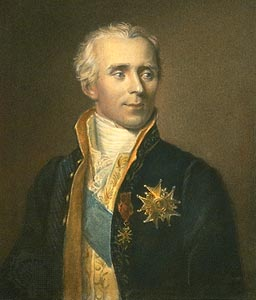
\includegraphics[width=0.3\textwidth]{graphic_files/Laplace_Pierre-Simon.jpg} \\
        Pierre-Simon, Marquis de Laplace (3 March 1749 – 5 March 1827) \\
    \end{center}
\end{frame}

\begin{frame}{Laplace Transform}
    \begin{alertblock}{Definition}
        The Laplace transform $F(s)$ of a function $f(t)$ is defined as $$\mathcal{L}\{f(t)\} = F(s) = \int_{0}^{\infty} f(t)e^{-st}dt,$$
        where $s = \sigma + j\omega$ is a complex variable
    \end{alertblock} 
    \begin{itemize}
        \item It transforms a \textbf{time-domain} $f(t)$ into a \textbf{complex frequency-domain} function $F(s)$ through the process of integration.
        \item The integration involves a ``kernel'' $k(s,t) = e^{-st}$, a function of both the complex variable $s$ and the time variable $t$ in the two spaces.
        \item The term $e^{-st}$ is sometimes called the ``convergence factor" which makes the integral converges for a wide range of functions.
    \end{itemize}
\end{frame}

\begin{frame}
    complex frequency-domain
    and then $h(t) = e^{-t}sin(t) = e^{\sigma t}sin(\omega t) = e^{\sigma t}e^{j\omega t} = e^{(\sigma + j\omega)t} = e^{st}$
    The Laplace transform of the Dirac delta function is 1 $\mathcal{L}[\delta(t)] = 1$, which simplifies the analysis of systems with impulsive inputs.
    Now it sees the system's response to a Dirac delta function as a unit function in the s-domain and see a unit step function as a 1/s function in the s-domain
    The Transfer Funcition is simply the Laplace transform of the system's unit impulse response
\end{frame}

\begin{frame}
    u(t) is the unit step function, telling that the input is applied at t=0 and the system is at rest before t=0
    so when it multiplies with the input, it will make sure that the input is zero before t=0
\end{frame}

\begin{frame}
    the Laplace transform make it easier to analyze the system's behavior in the s-domain.
    block diagram of the system in the s-domain with input, output, and transfer function
    description becomes algebraic equation in the s-domain, which is easier to solve than the ODE in the time domain
    from the idea of convolution integral, we can see that the output of the system is the convolution of the input and the impulse response
    in the s-domain, convolution becomes multiplication, which simplifies the analysis of systems with arbitrary inputs
\end{frame}

\begin{frame}
    Relating back to convolution integral, the Laplace transform of the convolution of two functions is the product of their individual Laplace transforms: $$\mathcal{L}\{f(t) * g(t)\} = F(s)G(s).$$
    $$ \mathcal{L}\{f(t) * g(t)\} = \int_{0}^{t} f(\tau)g(t-\tau) d\tau = \int_{0}^{t} g(\tau)f(t-\tau) d\tau= F(s)G(s)$$
\end{frame}


\begin{frame}
    Laplace transform table 
    loopback to the source of $h(t) = e^{-t}sin(t)$ from unit impulse response of the mass-spring-damper system
    showing the Laplace transform of the ODE and the solution in the s-domain and then inverse Laplace transform to get back to the time domain
    you get the same solution as before, but now you can see that the Laplace transform makes it easier to solve ODEs with arbitrary inputs
\end{frame}

\begin{frame}
    MATLAB DEMO: Laplace Transform and Inverse Laplace Transform
\end{frame}

\begin{frame}{Announcement}
    Form a group of 4 student and register for Mini-Lab 1
    Each group must bring a data cable (one end with USB-C to connect with the board) next week for the mini-lab session
    HW 1 (due 10 days after publishing) and Lab 1 Handout will be published this week
    Scan QR Code for providing feedback on lecture today
\end{frame}

\end{document}